\documentclass[twoside,a4paper]{report}

% rule: label after caption declaration

\makeatletter

% default packages
\usepackage[utf8x]{inputenc} % latex encoding
\usepackage[english, ngerman]{babel} % language support
\usepackage[T1]{fontenc} % coping umlaute in pdf

% layout & design
\usepackage[a4paper]{geometry} % page layout
\usepackage{setspace} % line spacing
\usepackage{fancyhdr} % custom header footer on pages
\usepackage{color} % colors font / background

% references
\usepackage{csquotes} % citing
\usepackage[backend=biber,style=apa,sorting=ynt]{biblatex} % bibliography / sources
\usepackage{pdflscape} % landscape pages
\usepackage[hidelinks]{hyperref} % named references
\usepackage[hyphenbreaks]{breakurl} % linebreaks in urls

% external files
\usepackage{import} % import latex in included files
\usepackage{graphicx} % images / graphics
\usepackage{pdfpages} % include pdf files

% tables
\usepackage{adjustbox} % scale down table
\usepackage[table]{xcolor} % color table parts
\usepackage[referable]{threeparttablex} % table with header & footer
\usepackage{multirow} % multi row cells in column
\usepackage{booktabs} % table rules / lines

% special elements
\usepackage{pifont} % special symbols
\usepackage{listings} % listings (also code snippets)
\usepackage{caption} % title in images 

% define colors - start
\definecolor{lgray}{rgb}{0.9, 0.9, 0.9}
\definecolor{dgray}{rgb}{0.3, 0.3, 0.4}
\definecolor{editorGray}{rgb}{0.95, 0.95, 0.95}
\definecolor{editorOcher}{rgb}{1, 0.5, 0}
\definecolor{editorGreen}{rgb}{0, 0.5, 0}
\definecolor{brown}{rgb}{0.69,0.31,0.31}
% define colors - end

% define symbols - start
\newcommand{\cmark}{\ding{51}} % ✓
\newcommand{\xmark}{\ding{55}} % ✗

\newcommand{\citemark}{\textsuperscript{[}\footnotemark\textsuperscript{]}} % [footnotemark]
\newcommand{\citemarktext}[1]{\textsuperscript{[}\footnote{#1}\textsuperscript{]}} % [footnote]
% define symbols - end

% define table styles - start
\newcommand{\tablesettings}[1]{\caption{#1} \smallskip \centering}
\newcommand{\trr}[1]{\multirow{-2}{*}{#1}} % double row
\newcommand{\trrr}[1]{\multirow{-3}{*}{#1}} % tripple row
\newcommand{\trrrr}[1]{\multirow{-4}{*}{#1}} % quarter row
\newcommand{\trrrrr}[1]{\multirow{-5}{*}{#1}} % quinter row
\newcommand{\ccgray}{\cellcolor{lightgray!60}} % gray cell

\newcommand{\tbbr}[1]{ % in table line break
  \begin{tabular}[l]{@{}l@{}}#1\end{tabular}
}
\newcommand{\trbbr}[3]{ % in multirow line break automatically
  \multirow{-#1}{*}{
    \hspace{-8pt} % remove too much space
    \renewcommand{\arraystretch}{0.8}
    \parbox{#2}{\raggedright #3}
    \renewcommand{\arraystretch}{1.1}
  }
}
\newcommand{\colwidth}{5cm} % default column width

\setlength{\tabcolsep}{4pt} % spacing table cell side
\renewcommand{\arraystretch}{1.1} % spacing table cell height
% define table styles - end

% define list of codes - start
\renewcommand{\lstlistingname}{Code} % name of caption
\renewcommand{\lstlistlistingname}{Codeverzeichnis} % name of listing
\newcommand{\codestyle}[1]{\texttt{\small #1}} % small code formatted text
% define list of codes - end

% define code styles - start
\lstdefinelanguage{js}{
  morekeywords={
    TODO, const, let, var, from, import, export, break, \{, \},
    case, catch, continue, debugger, default, else, \ as\ , \ =>\ ,
    false, finally, for(, for\ (, if(, if\ , in\ , instanceof, 
    new\ , null, return, switch, this, throw, true, \ try, typeof, void, while
  },
  morecomment=[s]{/*}{*/},
  morecomment=[l]//,
  morestring=[b]",
  morestring=[b]',
  morestring=[b]`
}
\lstdefinelanguage{html5}{
  language=html,
  sensitive=true,	
  alsoletter={<>=-},	
  morecomment=[s]{<!--}{-->},
  tag=[s],
  otherkeywords={
    % HTML tags
    <, </, >, />,     </a, <a, </a>,     </abbr, <abbr, </abbr>,     </address, <address, </address>,     </area, <area, </area>,     </area, <area, </area>,     </article, <article, </article>,     </aside, <aside, </aside>,     </audio, <audio, </audio>,     </audio, <audio, </audio>,     </base, <base, </base>,     </bdi, <bdi, </bdi>,     </bdo, <bdo, </bdo>,     </blockquote, <blockquote, </blockquote>,     </body, <body, </body>,     </br, <br, </br>,     </button, <button, </button>,     </canvas, <canvas, </canvas>,     </caption, <caption, </caption>,     </cite, <cite, </cite>,     </code, <code, </code>,     </col, <col, </col>,     </colgroup, <colgroup, </colgroup>,     </data, <data, </data>,     </datalist, <datalist, </datalist>,     </dd, <dd, </dd>,     </del, <del, </del>,     </details, <details, </details>,     </dfn, <dfn, </dfn>,     </div, <div, </div>,     </dl, <dl, </dl>,     </dt, <dt, </dt>,     </em, <em, </em>,     </embed, <embed, </embed>,     </fieldset, <fieldset, </fieldset>,     </figcaption, <figcaption, </figcaption>,     </figure, <figure, </figure>,     </footer, <footer, </footer>,     </form, <form, </form>,
    </h1, <h1, </h1>,     </h2, <h2, </h2>,     </h3, <h3, </h3>,     </h4, <h4, </h4>,     </h5, <h5, </h5>,     </h6, <h6, </h6>,     </head, <head, </head>,     </header, <header, </header>,     </hr, <hr, </hr>,     </html, <html, </html>,     </iframe, <iframe, </iframe>,     </img, <img, </img>,     </input, <input, </input>,     </ins, <ins, </ins>,     </kbd, <kbd, </kbd>,     </keygen, <keygen, </keygen>,     </label, <label, </label>,     </legend, <legend, </legend>,     </li, <li, </li>,     </link, <link, </link>,     </main, <main, </main>,     </map, <map, </map>,     </mark, <mark, </mark>,     </math, <math, </math>,     </menu, <menu, </menu>,     </menuitem, <menuitem, </menuitem>,     </meta, <meta, </meta>,     </meter, <meter, </meter>,     </nav, <nav, </nav>,     </noscript, <noscript, </noscript>,     </object, <object, </object>,     </ol, <ol, </ol>,     </optgroup, <optgroup, </optgroup>,     </option, <option, </option>,     </output, <output, </output>,     </p, <p, </p>,     </param, <param, </param>,     </pre, <pre, </pre>,     </progress, <progress, </progress>,     </q, <q, </q>,     </rp, <rp, </rp>,     </rt, <rt, </rt>,
    </ruby, <ruby, </ruby>,     </s, <s, </s>,     </samp, <samp, </samp>,     </script, <script, </script>,     </section, <section, </section>,     </select, <select, </select>,     </small, <small, </small>,     </source, <source, </source>,     </span, <span, </span>,     </strong, <strong, </strong>,     </style, <style, </style>,     </summary, <summary, </summary>,     </sup, <sup, </sup>,     </svg, <svg, </svg>,     </table, <table, </table>,     </tbody, <tbody, </tbody>,     </td, <td, </td>,     </template, <template, </template>,     </textarea, <textarea, </textarea>,     </tfoot, <tfoot, </tfoot>,     </th, <th, </th>,     </thead, <thead, </thead>,     </time, <time, </time>,     </title, <title, </title>,     </tr, <tr, </tr>,     </track, <track, </track>,     </u, <u, </u>,     </ul, <ul, </ul>,     </var, <var, </var>,     </video, <video, </video>,     </wbr, <wbr, </wbr>,     />, <!   }, 
  ndkeywords={    
    % HTML attributes
    accept=, accept-charset=, accesskey=, action=, align=, alt=, async=,      autocomplete=, autofocus=, autoplay=, autosave=, bgcolor=, border=,      buffered=, challenge=, charset=, checked=, cite=, class=, code=, codebase=,      color=, cols=, colspan=, content=, contenteditable=, contextmenu=,      controls=, coords=, data=, datetime=, default=, defer=, dir=, dirname=,      disabled=, download=, draggable=, dropzone=, enctype=, for=, form=,      formaction=, headers=, height=, hidden=, high=, href=, hreflang=,      http-equiv=, icon=, id=, ismap=, itemprop=, keytype=, kind=, label=,      lang=, language=, list=, loop=, low=, manifest=, max=, maxlength=,      media=, method=, min=, multiple=, name=, novalidate=, open=, optimum=,      pattern=, ping=, placeholder=, poster=, preload=, pubdate=, radiogroup=,      readonly=, rel=, required=, reversed=, rows=, rowspan=, sandbox=, scope=,      scoped=, seamless=, selected=, shape=, size=, sizes=, span=, spellcheck=,      src=, srcdoc=, srclang=, start=, step=, style=, summary=, tabindex=, target=,      title=, type=, usemap=, value=, width=, wrap=, popover=, popovertarget=,     
    % SVG attributes     
    fill=, attributeName=, begin=, dur=, from=, to=, poster=, controls=,      x=, y=, repeatCount=, xlink:href=,
    % CSS 
    background,background-attachment,     background-color,background-image,background-position,     background-position-x,background-position-y,background-repeat,     behavior,border,border-bottom,border-bottom-color,     border-bottom-style,border-bottom-width,border-collapse,     border-color,border-left,border-left-color,border-left-style,     border-left-width,border-right,border-right-color,     border-right-style,border-right-width,border-spacing,     border-style,border-top,border-top-color,border-top-style,     border-top-width,border-width,bottom,caption-side,clear,     clip,color,content,counter-increment,counter-reset,cue,     cue-after,cue-before,cursor,direction,display,elevation,     empty-cells,filter,float,font,font-family,font-size,     font-size-adjust,font-stretch,font-style,font-variant,     font-weight,height,ime-mode,include-source,     layer-background-color,layer-background-image,layout-flow,     layout-grid,layout-grid-char,layout-grid-char-spacing,     layout-grid-line,layout-grid-mode,layout-grid-type,left,     letter-spacing,line-break,line-height,list-style,     list-style-image,list-style-position,list-style-type,margin,   
    margin-bottom,margin-left,margin-right,margin-top,     marker-offset,marks,max-height,max-width,min-height,     min-width,orphans,outline,     outline-color,outline-style,outline-width,overflow,     overflow-X,overflow-Y,padding,padding-bottom,padding-left,     padding-right,padding-top,page,page-break-after,     page-break-before,page-break-inside,pause,pause-after,     pause-before,pitch,pitch-range,play-during,position,quotes,     richness,right,ruby-align,ruby-overhang,     ruby-position,-set-link-source,size,speak,speak-header,     speak-numeral,speak-punctuation,speech-rate,stress,     scrollbar-arrow-color,scrollbar-base-color,     scrollbar-dark-shadow-color,scrollbar-face-color,     scrollbar-highlight-color,scrollbar-shadow-color,     scrollbar-3d-light-color,scrollbar-track-color,table-layout,     text-align,text-align-last,text-decoration,text-indent,     text-justify,text-overflow,text-shadow,text-transform,     text-autospace,text-kashida-space,text-underline-position,top,     unicode-bidi,-use-link-source,vertical-align,visibility,     voice-family,volume,white-space,widows,width,word-break,     word-spacing,word-wrap,writing-mode,z-index,zoom
  }
}
\lstdefinestyle{htmlcssjs} {
  % General design
  backgroundcolor=\color{editorGray}, 
  basicstyle={\footnotesize\ttfamily},
  commentstyle=\color{red}, 
  frame=b,
  % Line numbers
  xleftmargin={0.75cm},
  numbers=left,
  stepnumber=1,
  firstnumber=1,
  numberfirstline=true,	
  % Code design
  identifierstyle=\color{black},
  keywordstyle=\color{blue}\bfseries,
  ndkeywordstyle=\color{editorGreen}\bfseries,
  stringstyle=\color{editorOcher}\ttfamily,
  commentstyle=\color{brown}\ttfamily,
  % Code
  language=html5,
  alsolanguage=js,
  alsodigit={.:;},	
  tabsize=2,
  showtabs=false,
  showspaces=false,
  showstringspaces=false,
  extendedchars=true,
  breaklines=true,
}
% define code styles - end

% page header and footer - start
% \rightmark = sub heading, \leftmark = chapter
\fancypagestyle{kolibri}{
    \setlength{\headheight}{17pt}

    \fancyhf{} % clear
    \fancyhead[RO]{\rightmark} % outer left page
    \fancyhead[LE]{\leftmark} % outer right page
    \fancyhead[C]{}
    \fancyhead[LO,RE]{} % inner
    \fancyfoot[LE,RO]{\thepage} % outer
    \fancyfoot[C]{
\includegraphics[width=16pt]{kolibri-logo2.png}}
    \fancyfoot[LO,RE]{
\includegraphics[width=25mm]{fhnw-logo.jpg}} % inner

    \renewcommand{\headrulewidth}{0.2mm}
    \renewcommand{\footrulewidth}{0.2mm}
    \renewcommand{\headruleskip}{2pt}
    \renewcommand{\footruleskip}{2pt}
}
\fancypagestyle{plain}{
    \setlength{\headheight}{17pt}

    \fancyhf{} % clear
    \fancyhead[LE,RO]{} % outer
    \fancyhead[C]{}
    \fancyhead[LO,RE]{} % inner
    \fancyfoot[LE,RO]{\thepage} % outer
    \fancyfoot[C]{
\includegraphics[width=16pt]{kolibri-logo2.png}}
    \fancyfoot[LO,RE]{
\includegraphics[width=25mm]{fhnw-logo.jpg}} % inner

    \renewcommand{\headrulewidth}{0mm}
    \renewcommand{\footrulewidth}{0.2mm}
    \renewcommand{\headruleskip}{0pt}
    \renewcommand{\footruleskip}{2pt}
}
\setlength{\headheight}{17pt}
% page header and footer - end

% define source folders - start
\graphicspath{ {./img/} }
\addbibresource{chapters/references.bib}
% define source folders - end

\newgeometry{inner=5cm, outer=2.5cm, top=3cm, bottom=3cm}
\setstretch{1.1}

% title page - start
\title{ Generalisierte Auswahlkomponente für das \\
Web UI Toolkit "Kolibri"\\ {\large Bachelor Thesis}}
\author{Ramona Marti \& Lea Burki}
\date{August 2024}
% title page - end

\makeatother

\begin{document}

\pagestyle{empty}

\begin{titlepage}

\includepdf[pages=-]{titlePage.pdf}
\end{titlepage}

% empty page
\newpage
\thispagestyle{empty}
\mbox{}
\newpage

\pagenumbering{Roman}
\pagestyle{kolibri}

% no numbering *
\chapter*{Abstract}

Die vorliegende Dokumentation beschreibt die Entwicklung einer plattformunabhängigen Dropdown-Komponente, die konsistent und benutzerfreundlich gestaltet ist. 
Die Hauptmotivation für diese Entwicklung ist, eine Komponente zu schaffen, die sowohl ästhetisch ansprechend als auch funktional ist. 
Sie lässt sich über verschiedene Webserver hinweg einheitlich nutzen. 
Die Komponente ist unabhängig von externen Bibliotheken entwickelt. 
Dazu basiert sie auf dem Kolibri-Designsystem, das als grundlegende Designrichtlinie dient. 

Wöchentlichen Meetings und die intensive Zusammenarbeit mit den Betreuern sind Bestandteile der gewählten, agilen Entwicklungsmethode. 
Diese Vorgehensweise überprüft den Fortschritt und plant das weitere Vorgehen. 
Die Testergebnisse zeigen, dass der Kolibri-Codestil eine kurze Einarbeitungszeit erfordert. 
Danach ist jedoch eine einfache Integration in Projekte als auch Anpassung der Komponente möglich. 

Ein besonderes Merkmal dieser Komponente ist die Möglichkeit, mittels mehrspaltiger Filterung eine gezielte Auswahl zu treffen. 
Die Vorauswahl eines Jahrzehnts ermöglicht die einfache Auswahl eines Geburtsjahres. 
Die Reduktion der Jahreszahlen minimiert das Scrollen und Suchen. 
Dieses Prinzip lässt sich analog für andere Anwendungsfälle – wie die Auswahl von Kontinenten \& Ländern oder spezifischen Mahlzeiten (z.B. vegetarische Gerichte) – anwenden. 

Für die Zukunft bietet die Komponente eine flexible Basis, die leicht zu erweitern ist. 
Zudem bestehen Potenziale für die Entwicklung ähnlicher Komponenten für weitere Anwendungsbereiche. 


% no numbering *
\chapter*{Ehrlichkeitserklärung}
\addcontentsline{toc}{chapter}{Ehrlichkeitserklärung}

Hiermit erklären wir, Ramona Marti und Lea Burki, dass wir unsere Bachelorarbeit mit dem Titel 
\textbf{24FS\_IMVS17: Generalisierte Auswahlkomponente für das Web UI Toolkit "Kolibri"} selbstständig und 
ohne unerlaubte Hilfe angefertigt haben. Wir haben keine anderen als die angegebenen Quellen und Hilfsmittel 
benutzt und alle wörtlich oder sinngemäss aus anderen Werken übernommenen Aussagen als solche gekennzeichnet. 
Diese Arbeit hat in gleicher oder ähnlicher Form noch keiner Prüfungsbehörde vorgelegen. 

\begin{center} 
      % nbsp here to remove error of newline at beginning of center
    \newline \newline \newline \newline

    Ort, Datum: \_\_\_\_\_\_\_\_\_\_\_\_\_\_\_\_\_\_
    \newline \newline \newline \newline 
    
    Unterschrift: \_\_\_\_\_\_\_\_\_\_\_\_\_\_\_\_\_\_
    \newline \newline \newline \newline 

    Unterschrift: \_\_\_\_\_\_\_\_\_\_\_\_\_\_\_\_\_\_
    \newline
\end{center}

% no numbering *
\chapter*{Danksagung}
\addcontentsline{toc}{chapter}{Danksagung}

Unser erster Dank geht an Prof. Dierk König und Fabian Affolter für die wertvollen Tipps und durchgehende Unterstützung 
während der Bachelorarbeit \textbf{24FS\_IMVS17: Generalisierte Auswahlkomponente für das Web UI Toolkit "Kolibri"}. 
Ihr Fachwissen und ihre Anleitungen haben entschieden zu unserer Lösung und dem Erfolg beigetragen. 

Zudem danken wir allen StudentInnen und FreundInnen, die sich als Test-Personen zu Verfügung gestellt haben. 
Sie haben uns mit konstruktiver Kritik und hilfreichen Anregungen Fehler und mögliche Erweiterungen aufgezeigt. 
Das Feedback hat uns inspiriert und Diskussionen mit unseren KommilitonInnen hat uns auf neue Ideen gebracht. 
Ohne sie hätte diese Arbeit nicht in dieser Form entstehen können. 

Weiter sprechen wir unseren Dank an unseren Familien und FreundInnen für ihre ständige Unterstützung und ihr Verständnis aus. 
Sie haben uns während des Studiums und der Fertigstellung dieser Arbeit motiviert unser Bestes zu geben. 
Ihre Geduld und ihre Ermutigungen haben uns geholfen die Konzentration zu halten und Kraft zu tanken. 
Sie haben während der ganzen Zeit ein offenes Ohr geboten und durch das Korrekturlesen zum Erfolg der Arbeit beigetragen. 

Zum Abschluss gilt unser Dank noch allen Personen, die uns im ganzen Studium als auch bei der Bachelorarbeit unterstützt haben. 
Ihre wertvollen Inputs, Hilfen und Motivationen beeinflussten den erfolgreichen Abschluss der Arbeit. 
Wir sind dankbar für diese Erfahrungen und all die Unterstützung und Anleitungen, die wir erhalten haben. 


\pagestyle{plain}
\tableofcontents

\newpage
\pagestyle{kolibri}
\pagenumbering{arabic}

\chapter{Einleitung}
\label{chap:intro}


\section{Problemstellung}
\label{sec:problem}

Im Web existieren diverse Möglichkeiten zur Erstellung eines Auswahl-Inputs mit vorgegebenen Werten. 
Die HTML-Elemente bieten über die verschiedenen Browser keine konsistente Darstellung und Interaktion an. 
Dazu sind sie nicht schön anzusehen und nur geringfügig anpassbar. 
Die Werte sind begrenzt auf Text und Unicode-Symbole. 
Die Komponente ist nicht effizient bedienbar – besonders bei einer grossen Menge an Werten. 

Als Alternative zu den Basiselementen existieren unzählige Bibliotheken, welche solche Eingabemöglichkeiten unterstützen. 
Diese besitzen externe Abhängigkeiten, welche das eigene Projekt unnötig aufblasen. 
Zudem benötigen viele dieser Libraries eine längere Einarbeitungszeit, um die Funktionalitäten verstehen und anwenden zu können. 
Das Vorgängerprojekt \textbf{Länderkomponente} deckt die Probleme ab, ist aber nur auf die Auswahl eines Landes zugeschnitten. 
Eine Anwendung dieser Komponente mit anderen Inhalten kann zu unerwünschtem Verhalten führen. 
Die oben genannten Probleme dienen als Basis für das folgende Kapitel. 


\section{Ziel}
\label{sec:goal}

Die neue Komponente \codestyle{SelectComponent} zielt darauf ab, die Auswahl eines Wertes aus einer begrenzten, vorgegebenen Menge zu ermöglichen.
Dazu finden die Generalisierung und der Ausbau der vorangegangenen Länderauswahl statt. 
Die Eingabe soll weiterhin effizient bleiben und sich konsistent über alle Browser zeigen. 
Dabei liegt der Fokus auf Browsern von Desktop-Computern bzw. Laptops. 
Die Komponente soll sich einfach anpassen lassen.
Als Werte sind nebst Texten auch Bilder wünschenswert. 
Die Qualität ist auf dem Kolibri-Standard zu halten und durch Tests zu beweisen. 
User-Tests mit Programmierern wie auch Endanwendern beweisen die gute Usability.
Automatisierte Komponententests stellen die Korrektheit der Implementation sicher. 
Bei der Umsetzung sollen die Design-Patterns des Kolibri ihre Anwendung finden. 
Dabei sollen das Design und die Interaktion mit dem Toolkit synchronisiert sein. 
Hierbei ist zu beachten, die Ziele nicht ausserhalb des Projekts zu definieren. 


\section{Out of Scope}
\label{sec:outOfScope}

Dieses Projekt bezieht sich auf die Entwicklung einer Auswahlkomponente für Nutzer ohne Seheinschränkungen. 
Daher spielt die Accessibility nur eine begrenzte Rolle. 
Screenreader sind nicht zu beachten, da dies zu umfangreich für diese Arbeit ist. 
Die effiziente Anzeige von übergrossen Datenmengen mit mehr als 10'000 Werten ist nicht verlangt. 
Die Eingabe eines eigenen Wertes in die neue Auswahlkomponente ist ebenfalls ausserhalb der Anforderungen. 
Für die generalisierte Komponente reicht es, wenn die Auswahl eines einzelnen Wertes möglich ist. 
Die Auswahl mehrerer Werte im selben Eingabeelement ist nicht gefordert. 
Die Komponente ist nicht speziell auf Mobile-Geräte auszurichten. 
Eine Undo- wie auch eine Redo-Funktion der ausgewählten Werte ist ausserhalb des geforderten Rahmens. 

Ein Bestandteil dieser Arbeit ist das Erweitern des \codestyle{SimpleInput}s um ein Select und eine Datalist. 
Damit der Fokus des Projekts auf der generalisierten Auswahlkomponente bleibt, sind keine Änderungen ausserhalb der oben genannten Ziele gefordert. 
Anpassungen der Kern-Codebasis gehören nicht in den Rahmen dieses Projekts. 
Die Eingrenzung der Anforderungen stellt sicher, dass die Ressourcen auf das Ziel fokussiert bleiben. 


\section{Leitfaden}
\label{sec:tocTexted}

Dieser Bericht gliedert sich in die Teile \textbf{Hintergrund}, \textbf{existierende} und \textbf{neue Komponenten} sowie die \textbf{Diskussion}. 
Jedes Kapitel baut auf dem Vorherigen auf und führt den Leser Schritt für Schritt durch die Entwicklung und Optimierung der neuen Auswahlkomponente. 

Im Kapitel \textbf{Hintergrund} (\textbf{\ref{chap:background}}) ist die \textbf{Ausgangslage} (\textbf{\ref{sec:basics}}) des Kolibri-Toolkits und des Projekts erläutert. 
Es folgt eine Erklärung der \textbf{Master-Detail-View} (\textbf{\ref{sec:masterDetailView}}). 
Nachfolgend sind die verschiedenen \textbf{Zustände} (\textbf{\ref{sec:states}}), die eine Auswahlkomponente besitzen kann, aufgeführt. 
Eine Beschreibung der \textbf{Browser und deren Rendering-Engines} (\textbf{\ref{sec:browserRenderer}}) ist ebenfalls enthalten. 
Der \textbf{Rendering-Prozess} einer HTML-Seite sowie die wichtigsten \textbf{Browser-Implementationen} sind ebenfalls auf dem Plan. 

Das Kapitel \textbf{existierende Komponenten} (\textbf{\ref{chap:existingComponents}}) vergleicht die \textbf{HTML-Elemente Datalist und Select} (\textbf{\ref{sec:datalistSelect}}). 
Die Nutzung und Unterschiede der verschiedenen Elemente sind hier ebenfalls beschrieben. 
Dabei hebt es die \textbf{Browser-Inkonsistenzen} (\textbf{\ref{sec:browserInconsistency}}) hervor. 
Sie führen zu \textbf{unterschiedlichen UI-Erfahrungen}. 
Die \textbf{Länderauswahl-Komponente} (\textbf{\ref{sec:countryChoice}}) aus der Vorarbeit ist nur auf die Auswahl eines Landes zugeschnitten. 
Mögliche \textbf{Anwendungsfälle} (\textbf{\ref{sec:useCases}}) der existierenden Komponenten zeigen die dabei entstehenden Probleme auf. 

Eine detaillierte Beschreibung der \textbf{neuen Komponente} findet sich im gleichnamigen Kapitel \textbf{\ref{chap:newComponent}}. 
Das \textbf{Design} (\textbf{\ref{sec:design}}) basiert auf dem Kolibri-Designsystem. 
Beim Visualisieren und Testen des neuen Designs kommen \textbf{Figma-Prototypen} zum Einsatz. 
Die \textbf{Implementation der Zustände} optimiert die Benutzerführung für Maus- und Tastaturbenutzer. 
\textbf{Prototyping und Benutzerfeedback} tragen in einem iterativen Prozess zur Verbesserung bei.
Das \textbf{Implementationsresultat} visualisiert und beschreibt die neue Komponente in diversen Beispielen.
Im Abschnitt \textbf{Interaktionen} (\textbf{\ref{sec:interaction}}) sind Regeln für die Maus- und Tastaturinteraktion festgelegt. 
Für einen stabilen und verständlichen Code sorgt die Einhaltung diverser \textbf{Prinzipien und Regeln} (\textbf{\ref{sec:principleRules}}). 
Der Einsatz von \textbf{Patterns} (\textbf{\ref{sec:patterns}}) wie \textbf{Null-Object}, \textbf{Projector} und \textbf{Decorator} strukturiert die Implementation. 
Die Patterns erhöhen die Wartbarkeit des Codes. 
Der \textbf{Dropdown-Container} (\textbf{\ref{sec:dropdownContainer}}) lässt sich auf verschiedene Weisen umsetzen. 
Das Kapitel \textbf{Performance} (\textbf{\ref{sec:performance}}) beschreibt Optimierungen zur Verbesserung der Ladezeit sowie des Leistungspotenzials der neuen Auswahlkomponente. 
Das \textbf{Testing}-Kapitel (\textbf{\ref{sec:testing}}) dokumentiert die Durchführung sowie die Auswertung von \textbf{manueller}, \textbf{automatisierter Tests} und \textbf{Usability-Tests}. 
Schliesslich fasst das \textbf{Fazit der neuen Komponente} (\textbf{\ref{sec:summeryNew}}) die wichtigsten Erkenntnisse zusammen. 

Abschliessend bietet die \textbf{Diskussion} (\textbf{\ref{chap:discussion}}) einen Überblick über die Bedeutung der Erkenntnisse für die Entwicklung. 
Zudem beschreiben die \textbf{Future Features} (\textbf{\ref{sec:future}}) Ideen für eine Weiterentwicklung sowie Verbesserungsvorschläge. 

\chapter{Hintergrund}
\label{chap:background}

Die Grundlagen stellen ein gemeinsames Verständnis der Auswahlkomponente her. 
Dazu zählen die Zustände, welche in diesem Zusammenhang auftreten können. 
Ausserdem behandelt es eine Basis zu den Themen Browser und Rendering. 
Dieses Verständnis ermöglicht es, eine neue, konsistente Komponente zu entwickeln.


\section{Ausgangslage}
\label{sec:basics}

Studenten wie auch Mitarbeiter entwickeln das Toolkit Kolibri laufend weiter. 
Entwickler können die Open-Source-Werkzeuge einfach importieren und verwenden.
Damit das Kolibri-Toolkit schlank bleibt, kommen keine externen Abhängigkeiten zur Verwendung. 
Mit einer VanillaJS-Codebasis bietet das Tool eine breite Auswahl an, deckt aber noch nicht alle Interaktionen ab. 

Der in der Vorarbeit hergestellte Fork dient als Ausgangslage.
Ein Merge – des Branches \emph{experimental} dieses Forks und des \emph{Kolibri-16} der originalen Codebasis – stellt die Aktualität sicher. 
Das \codestyle{SimpleInput} ist eines der Tools, welches sich bei der Implementation der neuen Auswahlkomponente als hilfreich erweisen kann. 

Die Vorarbeit\citemarktext{
    [\cite{ip5}]
} beinhaltet sowohl einen Recherche- als auch einen Design- und Implementationsbestandteil. 
Die Recherche legt den Fokus auf das Prototyping und diverse Code- und Implementationsbausteine. 
Die Anwendung der Informationen aus den Recherchen findet sich im Weg zur Länderauswahl wieder. 
Mehr zum Resultat dieser Arbeit folgt im Kapitel \textbf{\nameref{sec:countryChoice}}. 
Der komplette Bericht ist in der Quelle (\cite{ip5}) nachzulesen. 

Der Zugriff auf das Tool Figma ermöglicht das Verwenden des existierenden Designsystems und der bereits eingebundenen Elemente. 
Der Aufbau der Elemente als Komponenten vereinfacht die Wiederverwendung. 
Das Ergänzen des Icon-Sets ist bei Bedarf erlaubt. 

Eine weitere, wichtige Ausgangslage ist ein gemeinsames Verständnis der verwendeten Begriffe. 
Dies sicherzustellen, ist die Aufgabe des nächsten Kapitels mit der Beschreibung der Zustände einer Auswahlkomponente sowie deren Elemente. 
Diese Definitionen gelten im gesamten Bericht. 


\section{Master-Detail-Ansicht}
\label{sec:masterDetailView}

Eine Auswahlkomponente lässt sich unkonventionell in eine Master-Detail-Ansicht einteilen. 
Dies ist in Abbildung \ref{img:masterDetailView} ersichtlich. 

\begin{figure}[!htb]
    \centering
    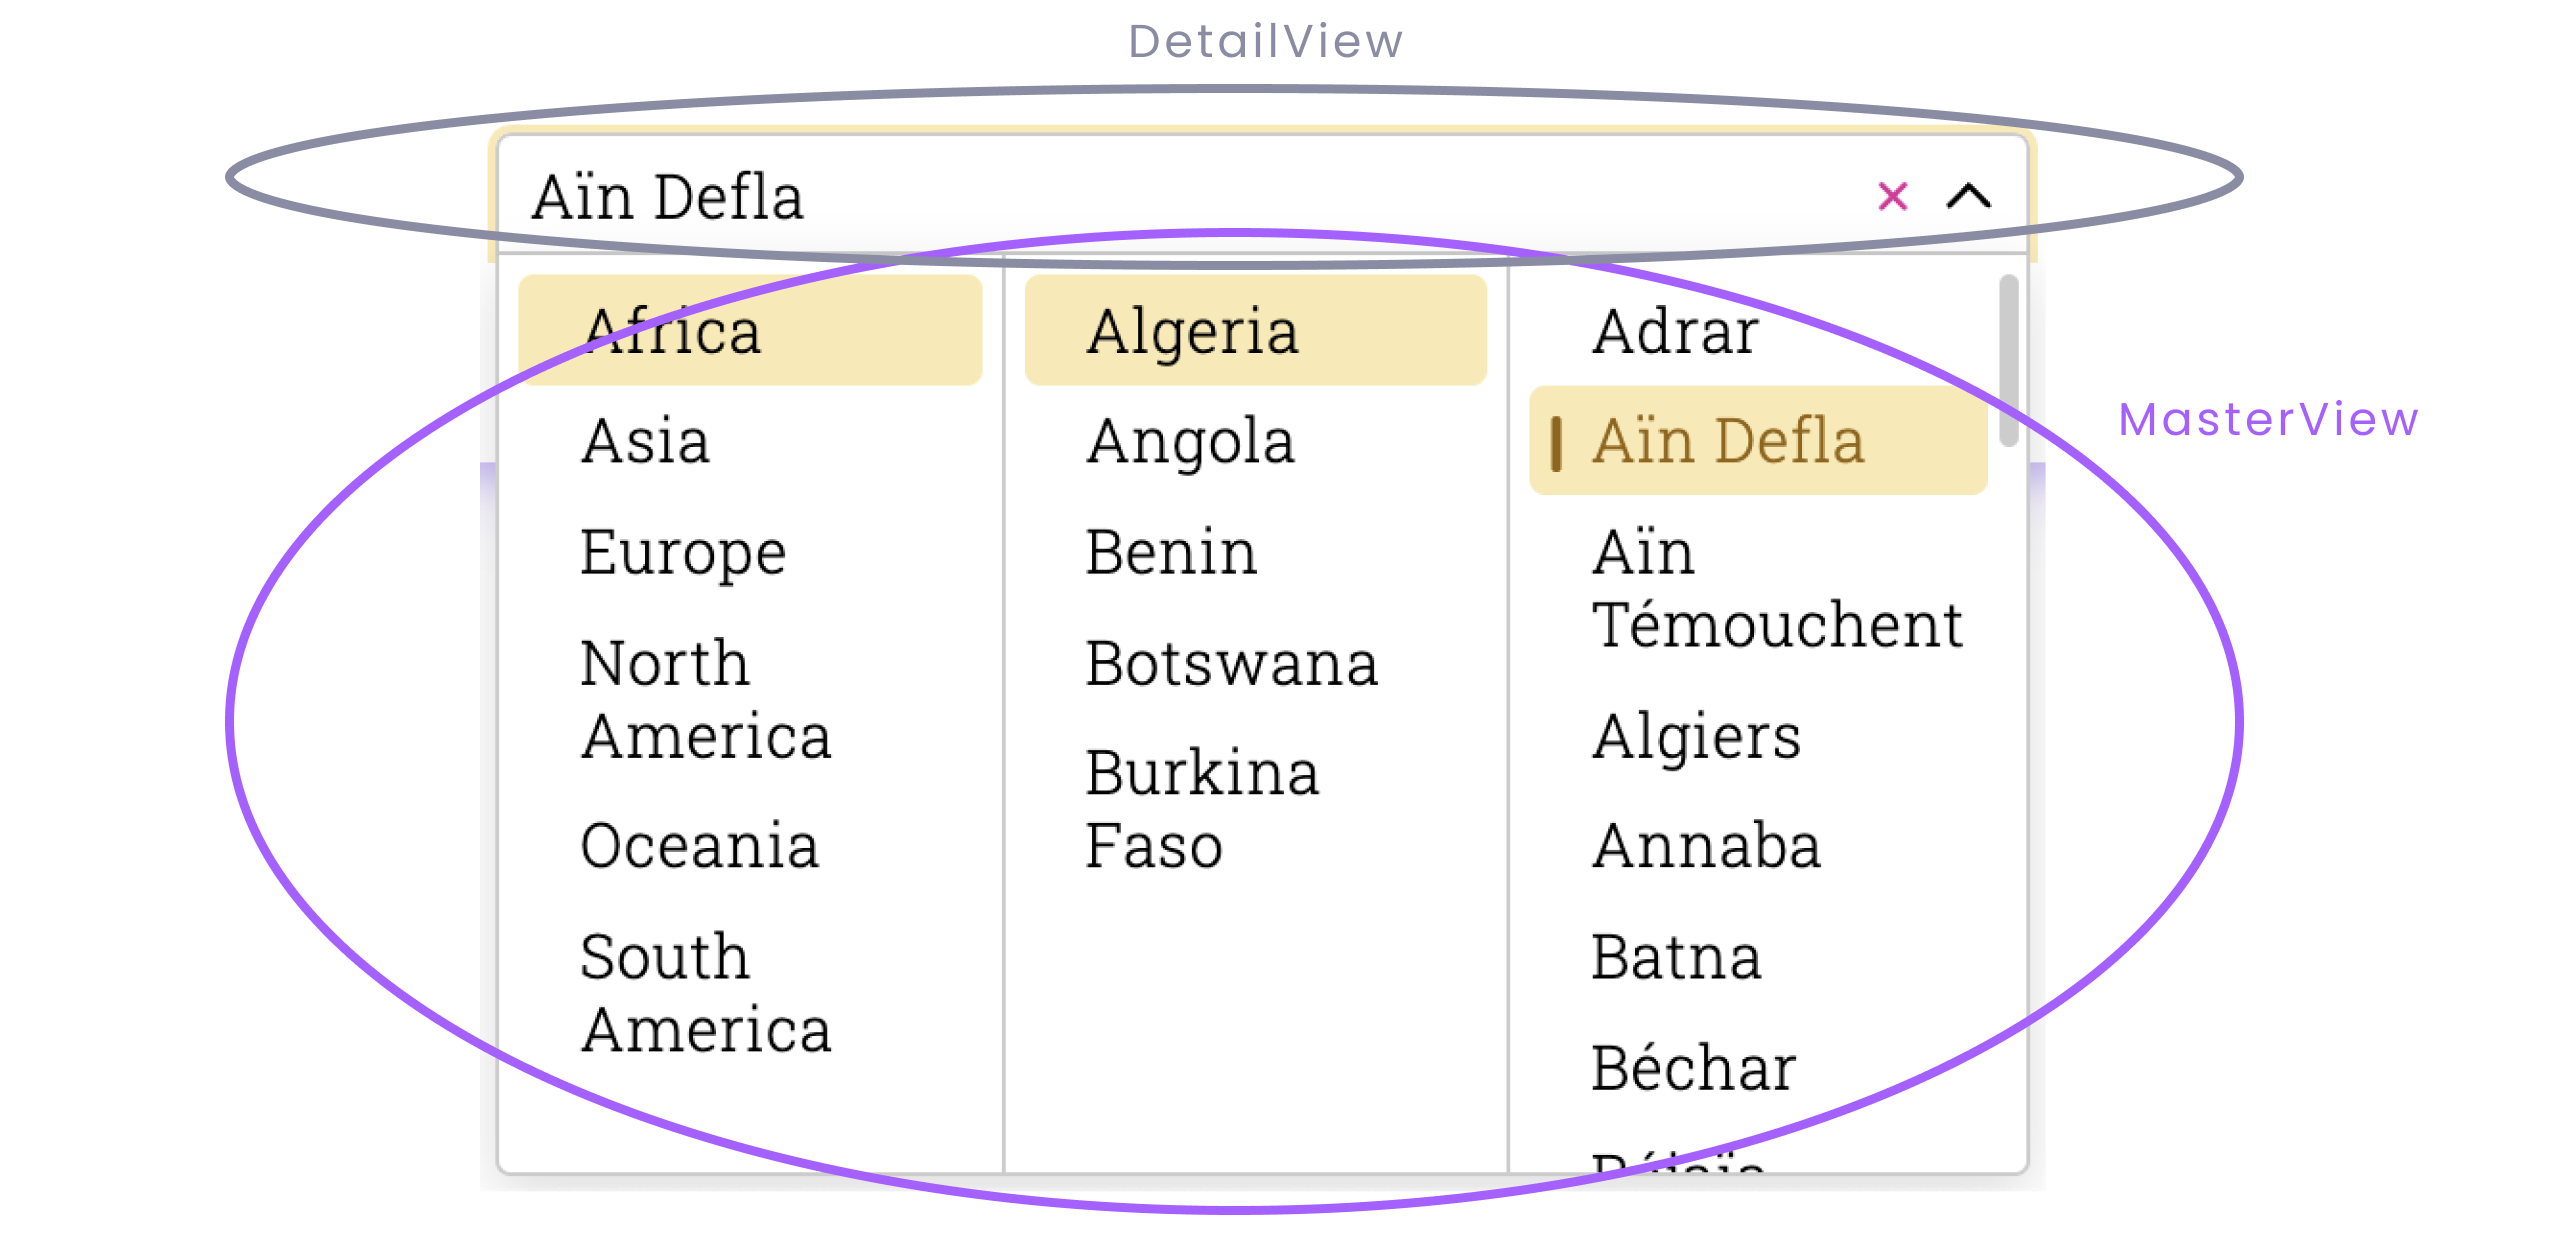
\includegraphics[width=80mm]{master-detail.png}
    \caption{\centering Master-Detail-Aufteilung der Auswahlkomponente}
    \label{img:masterDetailView}
\end{figure}

Typisch für die Master-Detail-View ist, dass die Detail-Ansicht mehr Daten anzeigt als der Master. 
Bei der Anwendung des Patterns auf eine Auswahlkomponente ist dies nicht der Fall. 
Anders als bei der typischen Master-Detail-View beinhaltet die Detail-Ansicht keine weiteren Informationen. 
Der Master listet alle möglichen Optionen auf. 
Dieser View-Baustein findet sich im aufklappenden, scrollbaren Container wieder. 
Die dauerhaft sichtbare Komponente stellt die Detail-View dar. 
Dieser Container beinhaltet sowohl den aktuell selektierten Wert als auch das Dropdown-Icon. 
Weiteres zu den möglichen Zuständen ist im nachfolgenden Kapitel zu finden. 


\section{Zustände in einer Auswahlkomponente}
\label{sec:states}

Dieser Abschnitt erklärt die Zustände, welche in einer Auswahlkomponente auftreten können. 
Als Ausgangslage dient eine Eingabemöglichkeit, die eine Master-Detail-Ansicht aufweist. 
Zudem sind keine speziellen Voreinstellungen getroffen. 

\begin{figure}[!htb]
    \centering
    \begin{minipage}[b]{0.4\textwidth}
        \centering
        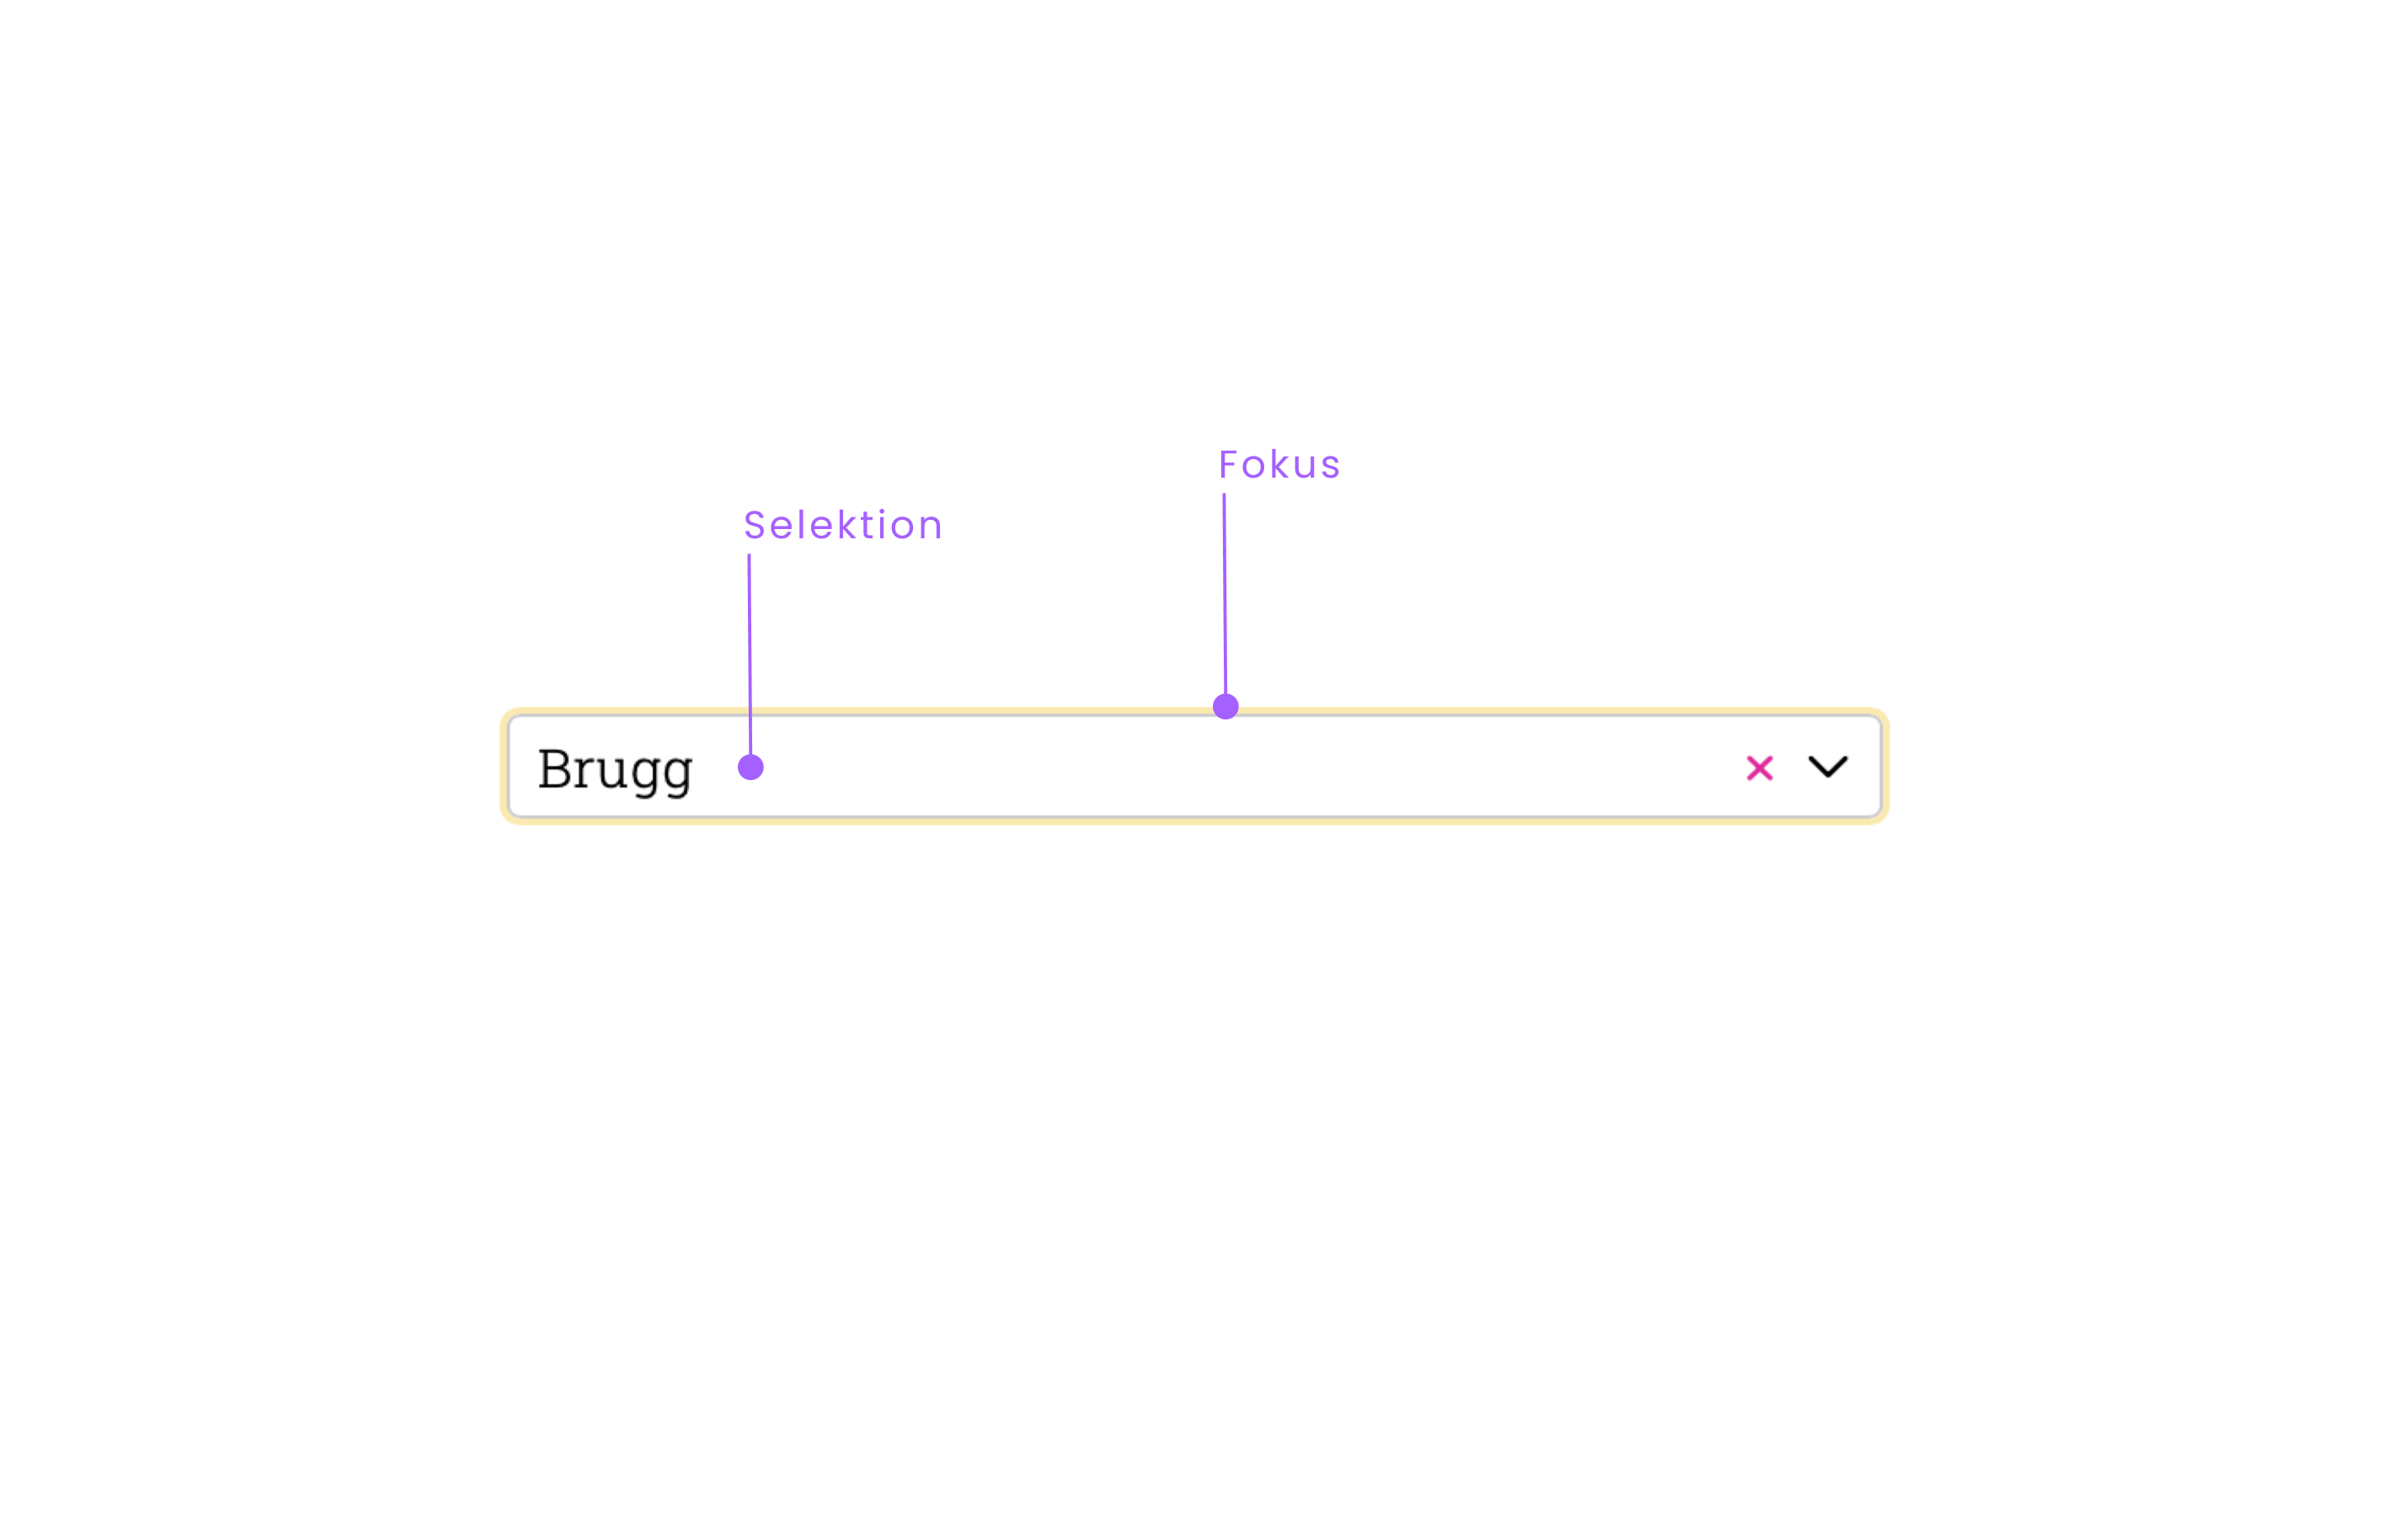
\includegraphics[width=\textwidth]{component-closed.png}
        \caption{\centering Geschlossene Komponente}
        \label{img:componentClose}
    \end{minipage}
    \hfill
    \begin{minipage}[b]{0.55\textwidth}
        \centering
        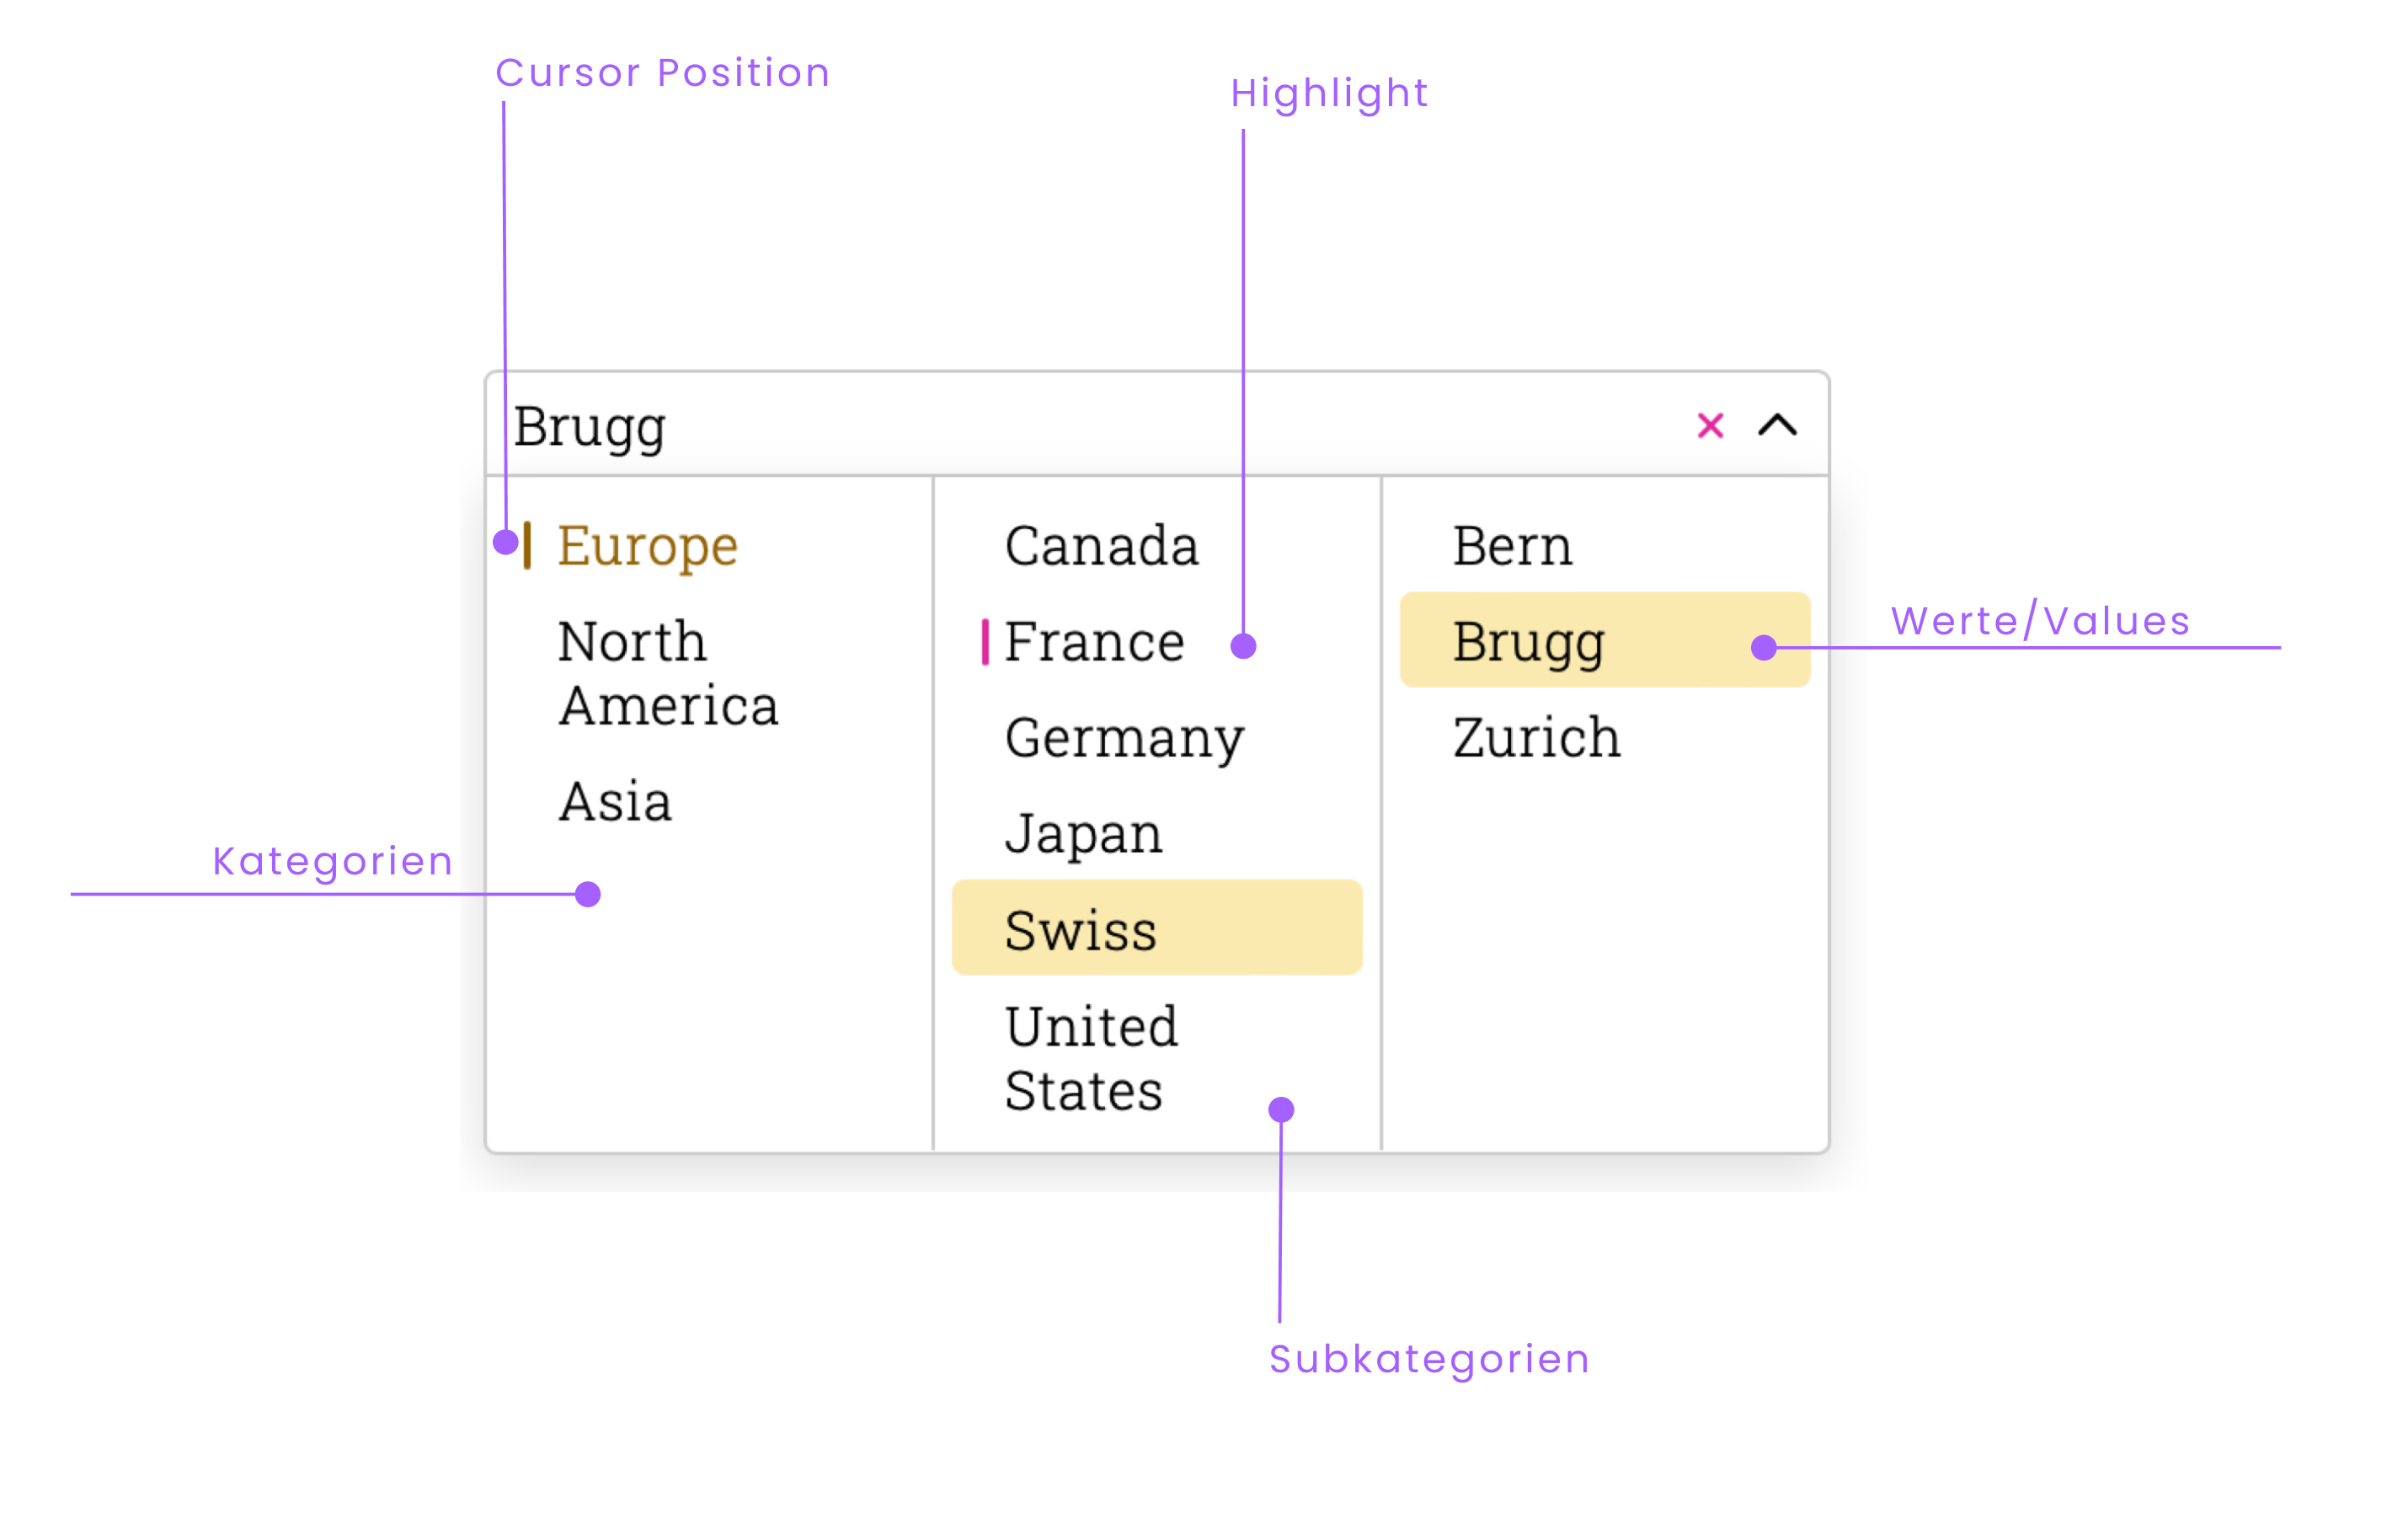
\includegraphics[width=\textwidth]{component-opened.png}
        \caption{\centering Offene Komponente}
        \label{img:componentOpen}
    \end{minipage}
\end{figure}

Je nach Darstellung der Komponente kann diese \emph{offen} oder \emph{geschlossen} sein. 
Im geschlossenen Status (Abbildung \ref{img:componentClose}) zeigt das Erscheinungsbild nur die Detail-Ansicht an.
Diese zeigt mindestens den selektierten Wert an. 
Eine offene Auswahlkomponente wie in Abbildung \ref{img:componentOpen} stellt beide Elemente der Master-Detail-View dar. 
Die Master-Ansicht zeigt alle Optionen in einer Liste an. 

Bei dem \emph{normalen} bzw. nicht fokussierten Status ist die Komponente nicht an- oder ausgewählt. 
Wenn eine Webseite diese Komponente enthält, ist dies die standardmässige Darstellung. 
Das neue Element zeigt keine Reaktion auf Interaktionen, welche in diesem Zustand geschehen. 
Als einzige Ausnahme gilt Tab, welche den Fokus auf die Komponente legen kann. 
In den meisten Erscheinungen ist nur die Detail-Ansicht sichtbar und der Master-Container ist ausgeblendet. 
Wählt der Nutzer die Komponente mit der Maus oder der Tastatur an, steht sie im \emph{Fokus} bzw. ist sie \emph{fokussiert}. 
Bedienungen über das Keyboard beziehen sich hierbei auf den Baustein. 
In den meisten Fällen ändert sich die Darstellung des Eingabefeldes – z. B. durch einen blauen Rahmen. 

Ist ein Wert in der Master-Ansicht ausgewählt und erscheint in der Detail-View, ist dieser \emph{selektiert}. 
Das Formular enthält beim Versenden das Value der \emph{Selektion}. 
Eine \emph{Selektion} in einer Kategorie-Spalte findet in den Formulardaten keine Berücksichtigung. 
Stattdessen filtert die Kategorie-Selektion die Wert-Spalte. 
Durch das Hervorheben zeigt sich in der Liste aller Werte eine getätigte Auswahl an. 
In gewissen Situationen existiert noch der Zustand, dass in der Master-View ein Wert im \emph{Highlight} steht. 
Bestätigt der Nutzer das \emph{Highlight} mit der Maus, wechselt der Status auf selektiert. 
Das Hovern kann den Highlight-Wert ändern. 
Geschieht die Navigation durch die Werte mit der Tastatur, erhält genau ein einzelner Wert die \emph{Cursor-Position}. 
Durch das Betätigen gewisser vordefinierter Tasten ändert sich die \emph{Cursor-Position}. 
Bei einer Bestätigung mit der Tastatur ändert sich der Wert der \emph{Cursor-Position} auf selektiert. 
Die letzten zwei Zustandswerte haben keinen Einfluss auf das versendete Formular. 
Sie sind nur im Master zu finden. 
Nachfolgend sind noch die Details zum Thema Browser erklärt. 


\section{Browser \& HTML-Renderer}
\label{sec:browserRenderer}

Die wichtigsten Aspekte von der Theorie über die populären Browser bis hin zum Ablauf des Renderings sind hier aufgeführt. 
Dabei sind nur die bekanntesten Implementationen von Belang. 

Ein Webbrowser dient als Zugang ins Internet und zur Anzeige von Webressourcen wie HTML, CSS und JavaScript. 
Er besteht aus einer Benutzeroberfläche, einer Browser- und einer Rendering-Engine. 
Für eine verständliche Darstellung der Inhalte auf dem UI verwendet die Browser-Engine einen sogenannten Renderer – mehr dazu später. 
Die Benutzeroberfläche dient als Schnittstelle zwischen dem Benutzer und der Datenschicht. 
Die Rendering-Engine interpretiert die Inhalte anhand des vorgegebenen Inhaltstyps. 
Einer der Engines ist der HTML-Renderer. 
Beim UI und der Bedienung zeigen sich die Uneinigkeiten zwischen den Browser-Herstellern. 
Der Grund liegt darin, dass die Rendering-Engine den Code nicht gleich interpretiert. 
Anschliessend sind Informationen über den detaillierten Ablauf zur Anzeige eines HTML-Dokuments und die Rolle des Renderings dokumentiert. 


\subsection{Rendering-Prozess}
\label{sec:structureRendering}

Der Aufruf einer Webseite beginnt mit dem HTTP-Request, auf welchen eine HTTP-Response folgt.
Die zuvor genannten Schritte vor der eigentlichen Datenerhebung sind in diesem Bericht nicht weiter von Bedeutung.
Der Response liefert letztlich die anzuzeigenden Daten, welche in diesem Fall die tragende Rolle spielen.

\begin{figure}[!htb]
    \centering
    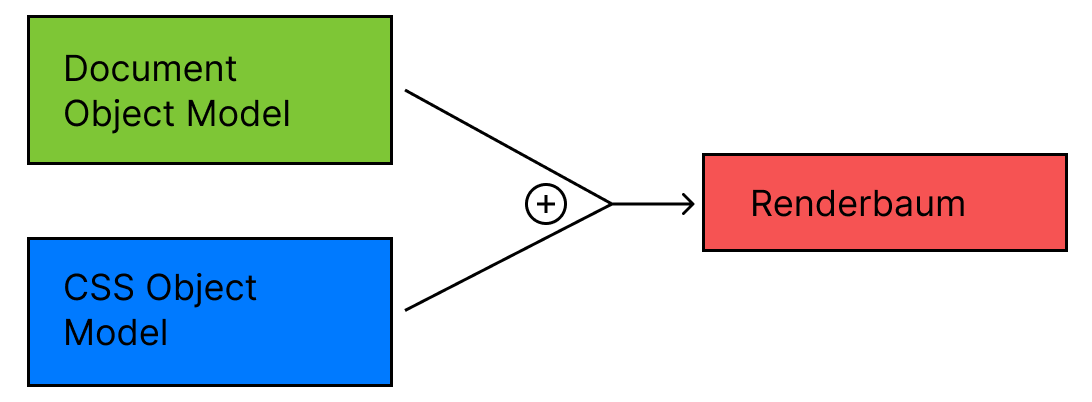
\includegraphics[width=80mm]{rendering-process.png}
    \caption{\centering Rendering-Prozess}
    \label{img:renderingProcess}
\end{figure}

Der Browser verarbeitet die erhaltenen Daten im HTML-Format weiter. 
Mehrere Schritte wandeln die einzelnen HTML-Elemente in sogenannte Nodes um. 
Aus den resultierenden Nodes entsteht durch Verknüpfungen eine Baumstruktur – der DOM. 
Das Document Object Model (DOM) (Abbildung \ref{img:renderingProcess} links oben) beschreibt die Eltern-Kind- und Geschwister-Beziehung der Nodes. 
Der Prozess bis zum CSS Object Model (CSSOM) gestaltet sich relativ ähnlich, ist aber nicht weiter wichtig. 

Der DOM und der CSSOM sind unabhängig voneinander.
Der Browser kombiniert die beiden Bäume zu einem gemeinsamen Renderbaum (Abbildung \ref{img:renderingProcess} rechts). 
Der resultierende Baum repräsentiert nur sichtbare Elemente, wohingegen der DOM alle Elemente enthält. 
Der Renderbaum ist browserabhängig. 

Dieses Wissen ist wichtig für das spätere Kapitel \textbf{\nameref{sec:performance}}. 
Der Grund ist, dass der Browser maximal 60 Mal pro Sekunde rendern kann. 
Jede Änderung am Browser-DOM\footnote{
    Im Renderbaum verwendeter und im Browser angezeigter DOM
} startet den kompletten Rendering-Prozess von vorne. 
Zu viele Änderungen am DOM führen dazu, dass der Nutzer länger warten muss, bis die Webseite geladen ist. 

Gründe für ein erneutes Rendern\citemarktext{
    [\cite{browserRendering3}]
}: 

\begin{itemize}
    \item Manipulation der Elemente des DOM
    \item Änderungen vom Inhalt (auch von Formularfeldern)
    \item Änderungen in den CSS-Eigenschaften
    \item Hinzufügen oder Entfernen von Stylesheets
    \item Ändern des Attributs \codestyle{class}
    \item Grössenänderung des Browserfensters
    \item Scrollen
    \item Pseudo-Klassenaktivierung
\end{itemize}


\subsection{Bekannte Implementationen}
\label{sec:implementationsRenderer}

Die neue Komponente soll in möglichst allen Browsern eine konsistente Erscheinung wie auch Interaktion bieten. 
Durch die Erklärung aus Kapitel \textbf{\nameref{sec:structureRendering}} ist klar, dass die Renderer die Unterschiede im UI bewirken. 
Die Bedienungsabweichungen stammen grösstenteils vom zugrunde liegenden Betriebssystem. 
Diese Erkenntnisse führen dazu, dass die neue Komponente auf Mac und Windows mit den geläufigsten Renderern zu testen ist. 
Zu den ausgewählten Webbrowsern zählen Google Chrome, Firefox (Mac und Windows), Safari (nur Mac) und Edge (nur Windows). 
Die Erläuterung dazu folgt im nächsten Abschnitt. 

Die populärsten Browser mit 65\% Marktabdeckung basieren auf der Chromium-Basis und verwenden alle den HTML-Renderer Blink\citemarktext{
    [\cite{blinkRenderer}]
}. 
Die Entwickler dieser Rendering-Engine sind die Open-Source-Community Chromium, Google, Intel und Samsung.
Zu den Browsern\citemarktext{
    [\cite{chromiumBrowser}]
}, die Blink als Rendering-Engine nutzen, gehören unter anderem Google Chrome, Brave, Microsoft Edge, Opera und Vivaldi. 
WebKit\citemarktext{
    [\cite{webkitRenderer}]
} – der Vorgänger des geläufigsten Renderers Blink – findet sich im OSX-Webbrowser Safari wieder. 
Diese von Apple, Google, KDE und Nokia entwickelte Rendering-Engine deckt 15\% ab. 
Firefox und weitere auf Mozilla basierende Browser\citemarktext{
    [\cite{mozillaBrowser}]
}, die Webseiten mit Gecko rendern, sind die bekanntesten Vertreter der verbleibenden Browser. 
Es existieren noch weitaus mehr Renderer, welche aber eine sehr geringe Verbreitung aufweisen. 
Deswegen sind diese nicht weiter von Belang.


% main chaapters here
\chapter{Existierende Auswahlkomponenten}
\label{chap:existingComponents}


Hier werden die bereits vorhandenen Möglichkeiten zur Darstellung einer Optionsauswahl einander gegenübergestellt.
Einer Auflistung der möglichen Funktionalitäten zeigt die Grenzen dieser Elemente auf.
Dabei spielen die UI- als auch die Interaktions-Unterschiede diese Komponenten in verschiedenen Browsern eine tragende Rolle.

Zu den bereits existierenden Komponenten zum Start dieser Arbeit zählen Buttons bzw. Links, \texttt{select}-, \texttt{datalist}-Element und das \texttt{Country Select}.
Unter dem Country Select ist das Resultat des Projekt 5 zu verstehen.
Die folgende Tabelle \ref{table:generalComparing} zeigt einen Vergleich der genannten Möglichkeiten.

\import{../tables}{c.choice.general.tex}


\section{HTML Datalist vs. Select}
\label{sec:datalistSelect}

Die folgenden Unterkapitel zeigen die Möglichkeiten, welche die HTML-Elemente \texttt{input}, \texttt{option}, \texttt{datalist} und \texttt{select} bieten.
Zudem zeigen tabellarische Gegenüberstellungen die Unterschiede und Inkonsistenzen dieser in verschiedenen Browsern und Betriebssystemen auf.
Hierbei liegt der Fokus mehr auf der Interaktion mit den Komponenten als auf der Darstellung.


\subsection{Option}
\label{sec:option}

\begin{lstlisting}[style = htmlcssjs, caption = Option Example, label = code:OptionExample]
<option value="ValueToSend">LabelToShow</option>
<option value="DefaultValue" selected>DefaultLabel</option>
<option value="Value" disabled>DisabledLabel</option>
\end{lstlisting}

Das \texttt{option}-Tag wird bei beiden Auswahlkomponenten - \texttt{datalist} und \texttt{select} - verwendet. 
Die einzelnen Optionen wie in Code \ref{code:OptionExample} Zeile 1 besitzen ein \texttt{value}-Attribut und einen Inhalt - das Label.
Alternativ kann das \texttt{label}-Attribut genutzt werden und der Value an die Stelle des Inhalts platziert werden.
Diese Variante wird jedoch von Firefox nicht unterstützt.
Werden \texttt{value} und \texttt{label} weggelassen, erhalten beide den Wert innerhalb des Tags.
Das HTML-Element kann das Attribut \texttt{disabled} oder \texttt{selected} erhalten.
Eine \texttt{selected} Option wie in Code \ref{code:OptionExample} Zeile 2 wird initial ausgefüllt und funktioniert nur im Zusammenhang mit dem \texttt{select}-Container. 
Bei einem \texttt{disabled} Element - wie in Code \ref{code:OptionExample} Zeile 3 - erscheint das UI ausgegraut.
Dieser Eintrag lässt keine Interaktion zu.

(\cite{optionMdn}) Das Designen von \texttt{option}s beschränkt sich auf die Text- / Hintergrundfarbe, welche jedoch nur in Firefox funktionieren. 
Die anderen Browser lassen kein Styling der Auswahl-Elemente zu bzw. zeigen diese nicht an.
Es ist nur ein skalarer Text als Inhalt erlaubt. 
Das bedeutet, es können keine weiteren Tags verschachtelt werden.
Als Eltern-Elemente sind \texttt{select}, \texttt{optgroup} und \texttt{datalist} erlaubt.
Alle gängigen Browser unterstützen dieses Tag.



\subsection{Select}
\label{sec:select}

\begin{lstlisting}[style = htmlcssjs, caption = Select Example, label = code:SelectExample]
<select name="animal">
    <option value="" disabled>Animal</option>
    <option value="dog">Dog</option>
    <option value="cat">Cat</option>
    <option value="mouse">Mouse</option>
</select>
\end{lstlisting}

Um den Wert zu speichern, benötigt das \texttt{select}-Tag ausser \texttt{option}s keine weiteren Elemente – ersichtlich im Code \ref{code:SelectExample}.
Die typischen Attribute für Eingabefelder wie \texttt{disabled}, \texttt{form}, \texttt{name} und \texttt{required} sind auch bei einem Select verwendbar.
Durch das \texttt{disabled} zeigt sich das Element in einer ausgegrauten Erscheinung und bietet dem Nutzer keine Interaktionsmöglichkeiten mehr.
Dieses Attribut kann vom Container - z.B. \texttt{fieldset} - geerbt werden.
Die \texttt{form}-Eigenschaft definiert das dazugehörige Formular und \texttt{name} den Key für das Key-Value Paar bzw. Name des Feldes im Formular. 
Mit dem \texttt{required} wird eine Eingabe erzwungen, um das Senden des Formulars freizuschalten.
Um dem Select für eine bessere Accessibility ein Label zuweisen zu können, ist eine \texttt{id} zu vergeben, 
Standardmässig ist für dieses Feld nur eine einzelne Auswahl möglich.
Durch die Ergänzung des Attributs \texttt{multiple} ist es möglich mehrere Werte zu markieren.
Bei einer Vorauswahl mehrerer Listenelemente durch \texttt{selected} muss die Komponente ein Multiselect sein.
Wenn jedoch bei einem Signle-Select mehrere Optionen das \texttt{selected}-Attribut enthalten, wird das Letzte als Default eingesetzt und die Vorherigen ignoriert.
Das \texttt{autocomplete} funktioniert wie bei anderen Inputs, indem Vorschläge vom User-Agent-Feature auftauchen.
Durch die \texttt{autofocus}-Eigenschaft sind Interaktionen mit dem Feld direkt nach dem Laden möglich.
Die Definition des \texttt{size}-Attributs steuert die Anzahl sichtbarer Elemente, wobei der Default für Single-Selects bei eins und mehrfache Auswahl bei vier liegt.
Ausser von dem \texttt{size}-Attribut erhält das Select von allen anderen in allen Browsern Unterstützung.
Die Grösse wird von den meisten Mobile-Browsern nicht supportet.

Abgesehen von der Grösse ist die Umgestaltung des Elements browserunabhängig kaum möglich.
Es gibt jedoch aufwendige Wege, den Inhalt zu klonen und durch Wrapper neu zu stylen.
In diesem Fall müssen aber die Logik und die Interaktionen für die Accessibility neu implementiert werden.
Gewisse Stylings können getroffen werden, wobei aber nicht alle Browser diese in der selben Weise übernehmen.
Durch die komplexe Struktur des Selects ist eine eigene Darstellung schwierig zu kontrollieren.

(\cite{selectMdn}) Der Inhalt des Tags können \texttt{option}s oder \texttt{optgroup}s sein.
Mehr zur \texttt{optgroup} kommt im nachfolgenden Unterkapitel.
In der ARIA-Rolle wird die Komponente als Combobox (ohne \texttt{size} \& \texttt{multiple}) oder Listbox gehandhabt.

Die mehrfache Auswahl rein per Tastatur bietet in der Interaktion geringere Möglichkeiten als mit der Maus.
Mit gedrückter Cmd (Mac) bzw. Ctrl (Windows) Taste können mit der Maus weitere Elemente mitausgewählt werden.
Mit dem Drücken der Shift-Taste lassen sich alle Elemente zwischen der ersten und der letzten Option markieren.
Damit sich die zuvor markierte Auswahl nicht aufhebt, ist darauf zu achten, beim Anwenden beider Techniken den Bereich mit Shift zuerst auszuwählen.
Um nur mit der Tastatur mehrere Werte zu markieren, ist es unabdingbar, zuerst zum ersten Element zu navigieren.
Mit Shift und den Pfeiltasten hoch und runter ist ein Bereich wählbar.
Firefox unterstützt noch die einzelne Mehrfachauswahl über die Tastatur, indem mit Ctrl der Fokus hoch und runter bewegt wird und mit der Leertaste selektiert werden kann.
Auf dem Mac sind die Tastenkombinationen Systembefehle.
Daher gibt es keine Alternative als sie zuvor auszuschalten bzw. umszustellen.


\subsubsection{\color{dgray} Optgroup}
\label{sec:optgroup}

\begin{lstlisting}[style = htmlcssjs, caption = Optgroup Example, label = code:OptgroupExample]
<select name="animal">
    <optgroup label="Big animal">
        <option value="dog">Dog</option>
        <option value="cat">Cat</option>
    </optgroup>
    <optgroup label="Small animal">
        <option value="mouse">Mouse</option>
        <option value="hamster">Hamster</option>
    </optgroup>
</select>
\end{lstlisting}

Die \texttt{optgroup} dient als Zusatz-Element um in \texttt{select}s Optionen zu Gruppieren und mit einem Zwischentitel zu versehen.
Der Titel lässt sich durch das \texttt{label}-Attribut setzen, ist aber nicht selektierbar. 
Um ein ganzer Block von Auswahlmöglichkeiten auszugrauen, bietet sich das \texttt{disabled} an.
Die Optionen, welche in diesem Tag enthalten sind, erben das Attribut.
Als Inhalt dienen \texttt{option}-Elemente und selbst besitzt es als Eltern-Tag ein \texttt{select}.
Die \texttt{optgroup} besitzt die ARIA-Rolle einer Gruppe und wird von allen Browsern unterstützt.


\subsection{Datalist}
\label{sec:datalist}

\begin{lstlisting}[style = htmlcssjs, caption = Datalist Example, label = code:DatalistExample]
<input type="text" name="animal" 
       list="data" placeholder="Animal" />
<datalist id="data">
    <option value="Dog"></option>
    <option value="Cat"></option>
    <option value="Mouse"></option>
</datalist>
\end{lstlisting}

Wie in Code \ref{code:DatalistExample} ersichtlich besteht die Datalist aus zwei Teilen - einem Input-Feld und einem Daten-Container. 
Im folgenden Unterkapitel \textbf{\nameref{sec:input}} wird detaillierter auf das Eingabefeld und dessen Typen eingegangen.
Die Datenliste besitzt keine speziellen eigenen Attribute.
Von den globalen Attributen sollte jedoch zumindest eine \texttt{id} vergeben werden.
Die Id dient zur Verknüpfung der Liste mit dem Input-Feld. 

(\cite{datalistMdn}) Das Stylen der \texttt{datalist} ist sehr begrenzt bzw. nicht möglich. 
Der Daten-Container reagiert nicht auf den Zoom des Browsers.
Gewisse Screenreader ignorieren die Vorschlagsliste und lesen diese somit nicht vor.
In der ARIA-Rolle wird das Element als Listbox interpretiert.

Die \texttt{option}s einer \texttt{datalist} besitzen normalerweise nur ein \texttt{value}-Attribut und kein Label oder nur Inhalt.
Bei einer zusätzlichen Label-Definition kann das je nach Browser zu abweichenden Darstellungen kommen. 
Während Firefox nur das Label in der Liste anzeigt, werden in den anderen Browsern Label und Value gemeinsam visualisiert. 
Die Browser, welche Label und Value anzeigen, heben den Wert ein wenig hervor.
Die Darstellung kann zu Missverständnissen führen, da bei der Auswahl nur das Value in das Eingabefeld eingefügt wird. 
Die \texttt{option}s-Werte können sich dem Typ des Inputs anpassen. 
Generell unterstützen alle Browser die \texttt{datalist}, aber Firefox nur begrenzt.

(\cite{datalistMdn}) Nicht alle Browser unterstützen die Datenliste für jeden Eingabe-Typ.
Der textuelle Typ funktioniert in allen Browsern und die Liste öffnet sich nach einem Klick bzw. Doppelklick auf das Feld.
Vordefinierte Datum- und Zeit-Typen funktionieren nur in den Chromium-basierten Browsern. 
Firefox und Safari zeigen den normalen Eingabe-Container, als ob die Liste nicht verknüpft ist.
Wenn eine Liste mit einer Range verwendet wird, zeigen alle Browser auf dem Slider die Optionen durch Markierungen an.
Die Kombination einer \texttt{datalist} mit einer Farbpalette zeigt eine breite, aber unterschiedliche Unterstützung. 
Unter den gängigen Browsern ist Firefox auf OSX der Einzige, welche die Liste nicht darstellt.
Zusammengefasst bieten für Listen mit den unterschliedlichsten Typen Chromium-basierte Browser die beste Unterstützung.


\subsubsection{\color{dgray} Input}
\label{sec:input}

Dieser Abschnitt behandelt nur den Teil, welcher im Bezug auf die \texttt{datalist} von Belang ist.
Das Input - in Code \ref{code:DatalistExample} auf Zeile 1 - wird durch das \texttt{list}-Attribut mit den Auswahloptionen verknüpft.
Bei der Verwendung zusammen mit der \texttt{datalist} ist dieses Attribut Pflicht.
Dadurch erscheinen die Auswahloptionen während der Bedienung des Input-Feldes. 

Die in diesem Kontext für alle Typen geltenden Attribute werden in diesem Paragraphen genauer behandelt.
Das \texttt{autocomplete}-Attribut dient zur Anzeige der Hinweise für das Autofill-Feature der Browser.
Das \texttt{disabled} schaltet die Interaktionsmöglichkeiten aus und deaktiviert somit die Komponente.
Ist das Eingabefeld ausserhalb eines Formulars platziert, lässt sich das Attribut \texttt{form} eine Verknüpfung zu einem auf der Seite existierenden Formular hergestellen. 
Im abgesendeten Formular dient die Eigenschaft \texttt{name} zur Identifizierung des Wertes im \texttt{value}-Attribut.
Der Typ des Eingabefeldes - angegeben durch das \texttt{type} - definiert, welche UI-Erscheinung das Input im Browser erhält und welche Werte zulässig sind.
Als Standard-Typ ist \texttt{text} definiert, wodurch dieses Attribut optional ist.
Mehr zu den für diese Arbeit wichtigen Typen ist im Unterkapitel \textbf{\nameref{sec:inutTypesDatalist}} zu lesen.
Die \texttt{id} als globale Eigenschaft dient bei den Eingabefeldern zusätzlich noch zur Verknüpfung mit einem Label-Element und somit einer bessern Accessibility.

Weiter existieren noch die zwei Attribute \texttt{readonly} und \texttt{required}, welche bei allen Typen ausser \texttt{range} und \texttt{color} definiert sind.
Durch die Ergänzung der ersten Eigenschaft ist der Wert nicht mehr änderbar, aber es bleibt im Verlauf der fokussierbaren Komponenten enthalten.
Das \texttt{required} erzwingt eine Eingabe.
Die Eigenschaften \texttt{min}, \texttt{max} und \texttt{step} unterstützen die Konfiguration der numerischen Typen\footnotemark.
\footnotetext{\texttt{date}, \texttt{month}, \texttt{week}, \texttt{time}, \texttt{datetime-local}, \texttt{number}, \texttt{range}}
Die ersten beiden begrenzen die Werte auf einen Bereich oder ein Intervall.
Mit \texttt{step} lässt sich noch die Grösse eines Schrittes einstellen.
Die textlichen Felder\footnotemark besitzen die Attribute \texttt{maxlength}, \texttt{minlength}, \texttt{pattern} und \texttt{size}.
\footnotetext{in diesem Zusammenhang: \texttt{text}, \texttt{search}, \texttt{url}, \texttt{tel}, \texttt{email}, \texttt{password}}
Diese Texttypen zusammen mit \texttt{number} können durch \texttt{placeholder} einen Patzhaltertext erhalten.
Die Min- und Max-Länge schränken die Textlänge der Eingabe ein.
Die Vorgabe eines Regex-Musters im \texttt{pattern}-Attribut kann die Eingabe weiter eingrenzen.
Das Formular validiert die Felder vor dem Senden anhand des Patterns und markiert fehlerhafte Einhaben als invalide.
Gewisse Typen - wie z.B. \texttt{url}, \texttt{tel} und \texttt{email} - haben bereits eine Pattern hinterlegt.
Mit \texttt{size} lässt sich die Grösse bzw. Anzahl sichtbarer Zeichen angeben.
Weitere Informationen zum Styling eines Input-Feldes stehen im Unterkapitel \textbf{\nameref{sec:inputCss}}.

Das Input enthält keinen Inhalt und ist ein selbst-schliessendes Tag.
Die ARIA-Rolle ist vom Typ abhängig und kann als Textbox, Combobox, Spinbutton, Slider, Searchbox, Telbox oder keiner speziellen Rolle zugeordent sein.
In den hier erwähnten Möglichkeiten der Kompontente existiert eine grossflächige Browserunterstützung.
Die einzigen Ausnahmen beziehen sich auf die Typen \texttt{week} und \texttt{month}, welche im Firefox und Safari nicht funktionieren.


\subsubsection{{\color{dgray} Input-Typen mit Datalist-Unterstützung}}
\label{sec:inutTypesDatalist}

(\cite{datalistMdn}) Bei den textuellen Typen existieren \texttt{text}, \texttt{search}, \texttt{number}, \texttt{email}, \texttt{url} und \texttt{tel}.
Diese Typen erscheinen als mehr oder weniger normales, einzeiliges Texteingabefeld.
Die ersten zwei der Auflistung verwalten einen Text ohne spezielle Anforderungen. 
Um die Werte als Zahlen zu speichern, dient der Typ \texttt{number}, welche dem UI noch zwei Buttons ergänzt.
Die letzten drei Typen sind Textfelder, welche bereits ein passendes Pattern für E-Mail, URL oder Telefonnummer hinterlegt haben.
Zudem zeigen diese Felder bei dynamischen Tastaturen eine der Situation angepasstes Layout\footnotemark.
\footnotetext{z.B.: @ und . ist bei \texttt{email} immer sichtbar, oder bei \texttt{tel} sind die Zahlen besser dargestellt}
Typen in der Kategorie Date-Time sind \texttt{month}, \texttt{week}, \texttt{date}, \texttt{time} und \texttt{datetime-local}.

Bei einer ungefähren Eingabe einer Zahl auf einem Intervall bietet sich \texttt{range} an.
Im UI zeigt sich diese Komponente als Slider, wobei sich der Standard Wert in der Mitte findet.
Zur Festlegung der Limiten dienen \texttt{min} und \texttt{max}.
Für eine Farbauswahl kann der Typ \texttt{color} zur Anwendung kommen. 
Die gängigen Browser zeigen nach dem Aufklappen Farbpaletten, welche sich aber in der Darstellung unterscheiden. 
Firefox beispielsweise greift auf die vom System gestellte Farbpalette zurück, wo Chromium-basierte Browser eine Eigene bieten.


\subsubsection{{\color{dgray} CSS für Input-Felder}}
\label{sec:inputCss}

(\cite{inputMdn}) Bei einem Input bestehen mehrere Möglichkeiten dieses umzugestalten.
Es existieren eigene CSS-Pseudo-Klassen, wobei folgend nur ein Teil aufgezählt wird.

\begin{itemize}
    \item \texttt{:enabled} bzw. \texttt{:disabled} - reagiert auf das \texttt{disabled}-Attribut
    \item \texttt{:read-write} bzw. \texttt{:read-only} - reagiert auf das \texttt{readonly}-Attribut
    \item \texttt{:valid} bzw. \texttt{:invalid} - reagiert auf die Client-Side Validität\footnotemark des Felds, sobald das Formular versendet wird
    \item \texttt{:user-invalid} - reagiert auf die Client-Side Validität des Felds, sobald das Feld verlassen wird
    \item \texttt{:in-range} bzw. \texttt{:out-of-range} - reagiert auf das \texttt{min}- und \texttt{max}-Attribut
    \item \texttt{:optional} bzw. \texttt{:required} - reagiert auf das \texttt{required}-Attribut
    \item \texttt{:blank} - reagiert wenn ein Feld leer ist
\end{itemize}
\footnotetext{Einhaltung der Regeln für das Input - z.B. ein gegebenes \texttt{pattern}}

Weiter gibt es noch das Pseudo-Element \texttt{::placeholder}, welches das Stylen des Platzhalters erlaubt.
Das CSS-Property \texttt{caret-color} färbt den Cursor\footnotemark in Inputs um.
\footnotetext{blinkender Strich in einem Eingabefeld}
Im Gegensatz zur \texttt{datalist} und dem \texttt{select} lässt sich das normale Eingabefeld relativ gut designen. 


\clearpage
\section{Browser-Inkonsistenzen}
\label{sec:browserInconsistency}

Die Komponenten Select \& Datalist variieren in der Ansicht als auch in der Interaktion. 
Die Unterschiede sind system-, browser- und komonentenabhängig. 
Nachfolgend sind die Inkonsistenzen genauer erläutert. 


\subsection{UI Unterschiede}
\label{sec:uiDifferences}

Das Select ist in der geschlossenen Form auf der rechten Seite immer mit mindestens einem Pfeil nach unten ausgestattet.
Safari (OSX und iOS) verwendet als Icon einen Doppelpfeil (nach oben und unten).
Firefox zeigt das Feld in grau, während alle anderen Browser einen weissen Hintergrund verwenden.
Safari auf iOS stellt die Komponente ohne Rahmen dar und deswegen ist der Hintergrund in einem hellen Grau gehalten.
Die geöffnete Liste ist bei Firefox als einziges relativ konsistent. 
Sie erscheint in einem mittel- bis hellgrauen Container.
Die anderen Browser sind einstellungsabhängig und zeigen den Container weiss oder dunkelgrau an.
Je nach Anzahl der enthaltenen Elemente erscheint die Liste darunter (darüber) oder überdeckt den Container des ausgewählten Wertes.
Am Wenigsten lässt sich das Element in Safari stylen.

Da nicht jeder Browser ein Icon anzeigt, ist die Datalist weniger konsistent.
Safari (Mac) und Firefox stellen keinen visuellen Hinweis auf einen Listen-Container dar.
Safari auf iOS zeigt hingegen in jedem Fall - bezogen auf den textuellen Typ - einen nach unten zeigenden Pfeil an.
Andere Browser blenden auf der rechten Seite beim Hovern oder beim Besitzen des Fokus das Icon (Dreieck nach unten zeigend) ein.
Bei Firefox unterscheidet sich das Öffnen der Liste ebenfalls. 
Wenn das Feld den Fokus noch nicht besitzt, benötigt es zwei Klicks.
Die anderen Browser lassen die Liste bereits beim ersten Kick erscheinen.
Die Liste selbst verhält sich je nach Browser und Inhalt verschieden, indem sie seitlich oder darunter (darüber) erscheint.
Ob der Dark- bzw. Light-Mode als Container-Farbe übernommen wird, ist vom Browser und dem Anwendungskontext abhängig.
Die Liste überdeckt der Eingabefeld nie. 

Ein Blick auf die mobilen Browser wie iOS-Safari, Android-Firefox und -DuckDuckGo zeigen weitere UI-Unterschiede.
Im Vergleich zu den Desktop-Version zeigen sich die geöffneten Selects auf Android für eine besser Bedienbarkeit in einem anderen Design.
Die Liste öffnet sich als Dialog-Popup und füllt je nach Anzahl der Werte fast den kompletten Display aus.
Das selektierte Element besitzt einen ausgefüllten Radio-Button auf der rechten Seite. 
Auf iOS-Browser erhält die ausgewählte Option ein Check-Icon (\cmark) auf der linken.
Der Listen-Container erscheint ähnlich zum OSX-Browser als Dropdown-Liste.
Nach einer Auswahl schliessen die mobilen Selects automatisch.

Die Datalist zeigt ihren Inhalt nur bei der Interaktion mit Pfeil auf der rechten Seite.
Abgesehen von der Grösse der einzelnen Einträge für die Bedienbarkeit unterscheiden die sich kaum von den Desktop-Versionen.
Die Selektionen erscheinen gegenüber der anderen Optionen in keinem speziellen Design.

Die nachfolgenden Abschnitte \textbf{\ref{sec:edgeBrowser}} bis \textbf{\ref{sec:mobileBrowser}} beschreiben die möglichen Interaktionen.
Die Tabellen stellen das Datalist, Single- als auch Multiselect einander gegenüber.
Im Anschluss an die Gegenüberstellungen der diversen Browser weist das Kapitel \textbf{\nameref{sec:summeryExisting}} detaillierter auf die Inkonsistenzen hin. 


\clearpage
\subsection{Edge Browser}
\label{sec:edgeBrowser}

\import{../tables}{c.edge.tex}

Auf Windows verhält sich Edge sehr ähnlich wie Chrome, da die Codebasis beider Browser Chromium ist.


\clearpage
\subsection{Chrome Browser}
\label{sec:chromeBrowser}

\import{../tables}{c.chrome.tex}

Auf dem Mac verhält sich Chrome ähnlich wie auf Windows, jedoch können sich Designaspekte unterscheiden. 


\clearpage
\subsection{Firefox Browser}
\label{sec:firefoxBrowser}

\import{../tables}{c.firefox.tex}

Wie auch auf Windows zeigt Firefox auf dem Mac konsistentes Verhalten, jedoch mit typischen OSX Designanpassungen. 
Die Interaktions-Feedbacks auf Mac können sich leicht von der Windows-Version unterscheiden.


\clearpage
\subsection{Safari Browser}
\label{sec:safariBrowser}

\import{../tables}{c.safari.tex}

Safari tendiert dazu, ein minimalistisches Design zu verwenden, was sich in der Darstellung von Dropdowns und Comboboxen widerspiegelt.
Dieser Browser verwendet Designelemente wie Schatten und Ränder in anderer Form als Chrome und Firefox.
Das Select zeigt die grössten Unterschiede im UI.


\clearpage
\subsection{Browser auf Android \& iOS}
\label{sec:mobileBrowser}

\import{../tables}{c.firefox.android.tex}
\import{../tables}{c.duckduck.android.tex}

Der Vergleich der Tabellen \ref{table:interactionFirefoxAndroid} und \ref{table:interactionDuckduckAndroid} zeigt, dass auf dem selben Android-Gerät Abweichungen existieren.
Nicht alle Bedienungsmöglichkeiten führen zur selblen Reaktion.

\clearpage
\import{../tables}{c.safari.ios.tex}

Wie in den Tabellen \ref{table:interactionFirefoxAndroid} bis \ref{table:interactionSafariIos} zu sehen ist, erlauben Mobilgeräten weniger Interaktionen als Desktop-Computer.
Zum einen stellen die verschiedenen virtuellen Tastaturen eine geringere Auswahl an Interaktionen an.
Auf der anderen Seite öffnet sich die virtuelle Tastatur nicht in jeder Situation. 
In Bezug auf die Komponenten Select und Datalist öffnet sich die dynamische Eingabemöglichkeit nur durch das Input der Datalist.
Dies ist der Grund, wieso in den drei oben dargestellten Tabellen keine Tastatur-Interaktionen bei Selects möglich sind. 
Die Unterschiede bei der Datalist entstehen dadurch, dass nicht jeder mobile Browser die Liste bei Tastatur-Eingaben offen lässt bzw. öffnet.
Dadurch erklären sich die unterschiedlichen Verhaltensweisen, welche in den Tabellen ersichtlich sind.

Die Touch-Bedienungen auf der Datalist weisen kaum eine Übereinstimmung auf. 
Das Scrollen als auch das Klicken verhalten sich bei den ausgewählten Mobile-Browsern Safari, Firefox und DuckDuckGo unterschiedlich.
Das Select zeigt sich in der Interaktion mit dem Finger konsistenter. 


\clearpage
\subsection{Fazit}
\label{sec:summeryExisting}

% todo rewrite with focus on differences visible in tables
Generell ändern sich in Bezug auf Design und Interaktionsmechanismen die Verhaltensweisen der Standardkomponenten in den verschiedenen Browsern. 
Hierbei spielen das betriebssystemspezifische Styling und die individuellen Implementierungen der Browser eine Rolle. 
Die Grundfunktionen zeigen sich ähnlich, wobei etwaige Unterschiede oft in der visuellen Darstellung und in Details der Interaktion (z.B. beim Öffnen der Dropdowns oder der Navigation innerhalb der Listen) liegen. 
Um eine optimale Benutzererfahrung bieten zu können, ist die Konsistenzprüfung unabdingbar.
Es ist die Sicherstellung, dass Webanwendungen über verschiedene Plattformen und Browser hinweg einheitlich funktionieren. 
Das Verhalten kann je nach Browserversion und Betriebssystem variieren. 
Die Analyse der Tabellen unterstreicht, dass trotz grundlegender Übereinstimmungen in der Funktionsweise von Komponenten wie Datalist und Select, 
die optische Darstellung und bestimmte Interaktionsdetails je nach Betriebssystem und Browser variieren. 
Insbesondere sind solche Unterschiede in der Bedienung mit Tastaturkürzeln wie Cmd/Ctrl und der Visualisierung von Navigationspfeilen oder Scroll-Verhaltensweisen sichtbar. 
Diese Erkenntnisse fordern eine sorgfältige Abstimmung und eventuelle Anpassungen im Designprozess, um eine einheitliche Benutzererfahrung sicherzustellen.


\section{Anwendungsfälle}
\label{sec:useCases}

Die existierenden Auswahlkomponenten finden in vielen Webapplikationen Anwendung.
Das bekanneste Beispiel eines Selects ist die Auswahl des Geschlechts.
Diese Verwendung ist abgesehen vom Design unproblematisch.
Ein anderer Anwendungsfall ist die Auswahl eines Jahres oder Geburtstags mit drei Selects.
Das Ausfüllen dieser Situation gestaltet sich schon unangenehmer.
Dies liegt daran, dass die Suche nach dem gewünschten Wert besonders beim Jahr eher lange dauern kann.
Besonders mühsam gestaltet sich für Nutzer die Suche nach dem Herkunfts- bzw. Zielland aus einer Liste von ca. 250 weltweit.
Aber auch den Wohn- oder Destinationsort aus mehreren 100 bis 1'000 (je nach Anwendungsgebiet) auswählen zu müssen, ist sehr zeitaufwendig.
Um die Anwendung angenehmer zu gestalten, bietet sich auf den ersten Blick die Datalist mit der eingebauten Filterfunktion an.
Das Problem ist jedoch, dass in den meisten Fällen eigene Eingaben unerwünscht sind.
Als ebenfalls schlechte alternativ bietet sich das Select als Auswahlkomponente an.
Damit zieht sich die Suche nach einem bestimmten Wert in die Länge - speziell wenn die Optionen nicht in alphabetischer Reihenfolge vorliegen.
Selbst die Zuhilfenahme der Select-Suche\footnotemark ist nicht in jeder Situation hilfreich. 
\footnotetext{Durch das Drücken der Anfangsbuchstaben des gesuchten Werte springt die Selektion zur passenden Option}
Ein weiteres Anwendungsgebiet findet sich in gewissen Webshop bei den Filter- und Sortierfunktionen wieder.
Die Komponente zeigt sich unter anderem bei der Auswahl einer Grösse, Farbe oder Kategorie.
In diesem Beispiel können viele Optionen bzw. Werte ohne klare Reihenfolge in einer Liste auftauchen.
Dies führt dazu, dass das Auffinden des gewünschten Werts eher schwer fällt.
All die oben genannten und noch weitere Fälle zeigen verschiedene Probleme auf.
Die neue Komponente ermöglicht es, die unangenehmen Situationen aufzulösen.
Mehr Informationen dazu ist im nachfolgenden Kapitel zu lesen.

\chapter{Neue Auswahlkomponenten}

% todo paragraph
{\color{red} \textbf{FEHLENDER PARAGRAPH KOMMT NOCH}}


\section{Design}

Das Design der neuen Auswahlkomponente ist stark vom Kolibri-Designsystem inspiriert, jedoch mit einigen Anpassungen, um die Lesbarkeit und Benutzerfreundlichkeit zu optimieren. 
Der Fokus liegt darauf, eine konsistente und ansprechende Benutzererfahrung zu schaffen, die sich über alle modernen Browser hinweg hält.


\subsection{Designansatz}

Die Gestaltung der Dropdown-Komponente basiert auf dem Designsystem Kolibri, um eine konsistente Benutzererfahrung zu gewährleisten. 
Kolibri bietet bereits ein umfassendes Set von Richtlinien und Komponenten, die es ermöglichen, Anwendungen einheitlich und benutzerfreundlich zu gestalten.


\subsection{Mögliche Designoptionen eines Elements \& deren Wahl}

Elemente lassen sich durch diverse Eigenschaften stylen.
Die Anpassung der Hintergrundfarbe fällt am schnellsten ins Auge.
Diese ist hell zu gestalten, damit der Kontrast zur dunklen Default-Schriftfarbe erhalten bleibt.
Der Rahmen bietet eine weitere Designmöglichkeit. 
Seine Farbe, Dicke oder Struktur kann varriieren. 
Eine andere Alternative ist nur eine Seite des Rahmens zu verwenden. 
Als Beispiel dafür gilt der sogenannte Spiegelstrich, welcher beispielsweise auf der linken Seite platzierbar ist.
Die Färbung Rund um den Rahmen sollte für einen gute Erkennbarkeit in einer eher dunklen Schattierung Anwendung finden.
Als weitere Style-Eigenschaften bietet sich Änderungen der Schrift an.
Bei der Farbe ist der Kontrast zu beachtet, weswegen eine eher Dunkle zu wählen ist.
Alternativ lässt sich die Dicke, Schriftart, Neigung, Grösse oder Dekoration ändern.
All diese Style-Anpassungen lassen natürlich auf verschiedene Weise kombinieren.

Bei den Farben existiert eine grosse Bandbreite.
Da Kolibri bereits ein Designsystem besitzt, schränkt sich die Menge ein.
Unter den vorhandenen Farbwerten, bieten sich die folgenden am besten an:

\begin{itemize}
    \item Kolibri-Light/Yellow/100 $\rightarrow$ helles Weiss-Gelb
    \item Kolibri-Light/Yellow/300 (--kb-color-select) $\rightarrow$ helles Gelb
    \item Kolibri-Light/Warning/--kb-warning-dark $\rightarrow$ dunkles Gelb
    \item Kolibri-Light/Danger/--kb-danger-accent (--kolibri-color-accent) $\rightarrow$ mittleres Rosa
    \item Kolibri-Light/Success/--kb-success-accent $\rightarrow$ mittleres Grün
    \item Kolibri-Light/Success/--kb-success-light $\rightarrow$ helles Grün
    \item Kolibri-Light/Primary/--kb-primary-accent $\rightarrow$ mittleres Violet
    \item Kolibri-Light/Primary/--kb-primary-light $\rightarrow$ helles Violet
    \item Kolibri-Light/Secondary/--kb-secondary-accent $\rightarrow$ mittleres Blau
    \item Kolibri-Light/Secondary/--kb-secondary-light $\rightarrow$ helles Blau
    \item Kolibri-Light/Monochrome/--kb-color-body $\rightarrow$ mittleres Grau
    \item Kolibri-Light/Monochrome/--kb-color-line $\rightarrow$ helles Grau
\end{itemize}

Da die Elemente drei verschiedene Zustände gleichzeitig erhalten können, müssen die Styles kombinierbar sein.
Nicht jede der erwähnten Eigenschaft und Farb eigent sich in gleichem Masse.
Yellow-100 fällt schnell wieder weg, da je nach Display der Kontrast zu gering ist.
Unter den restlichen hellen Schattierungen passt Yellow-300 am besten, da diese Farbe bereits als Selektionsfarbe im Code hinterlegt ist.
Das vordefinierte $--kb-color-select$ eignet sich am ehesten als Hintergrundfarbe.
Dadurch ist klar, dass die anderen beiden Zustände eine eher kräftige bzw. dunkle Färbung benötigen.
Der Blick auf die Namen im Designsystem zeigt eine weitere Farbe zur Hervorhebung eines Elements.
Die Benennung des mittleren Rosa mit Accent ($--kolibri-color-accent$) bietet einen guten Kontrast zur Selektion und ist ebenfalls im Code vordefiniert.
Da die dritte Farbe nicht zu viel Unruhe in das Design bringen soll, schränkt sich die Farbauswahl weiter ein.
Mit einem gut erkennbaren Kontrast zur Selektion bietet sich das dunkle Gelb aus $--kb-warning-dark$ an.

Wie erwähnt ist die Eigenschaft Hintergrundfarbe durch die Wahl der Farbe bereits festgelegt. 
Die Schrift sollte maximal in der Farbe geändert werden. 
Weil die anderen Styling-Optionen sind schwer erkennbar oder zerstören das Bild.
Der komplette Rahmen passt nicht in das Design und fällt somit ebenfalls weg.
Da nicht beide Zustände auf die Schriftfarbe zugreifen können, bietet sich der oben genannte Spiegelstrich an.
Das Rosa mit dem grösseren Kontrast erhält nur linken Rahmen.
Das dunkle Gelb färbt - nebst dem linksseitigen Strich - die Schrift.
Die Zuordnung der Designwahl zu den fehlenden Zuständen steht im Kapitel \textbf{Farbpalette und Kontrast}.


\clearpage
\subsection{Figma-Prototypen}

Zur Visualisierung und interaktiven Testing des Designs kam Figma zum Einsatz. 
Figma ist ein webbasiertes Tool zur Erstellung von UI/UX-Designs, das Echtzeit-Kollaboration ermöglicht. 
Durch die Nutzung von Figma konnten schnell Prototypen erstellt und diese mit Stakeholdern und Nutzern geteilt werden, um Feedback zu sammeln und Iterationen vorzunehmen.

Die folgenden Screenshots \ref{img:figmaPrototype1} bis \ref{img:figmaPrototype3} zeigen die in Figma erstellten Prototypen der Dropdown-Komponente:

\begin{figure}[!htb]
    \centering
    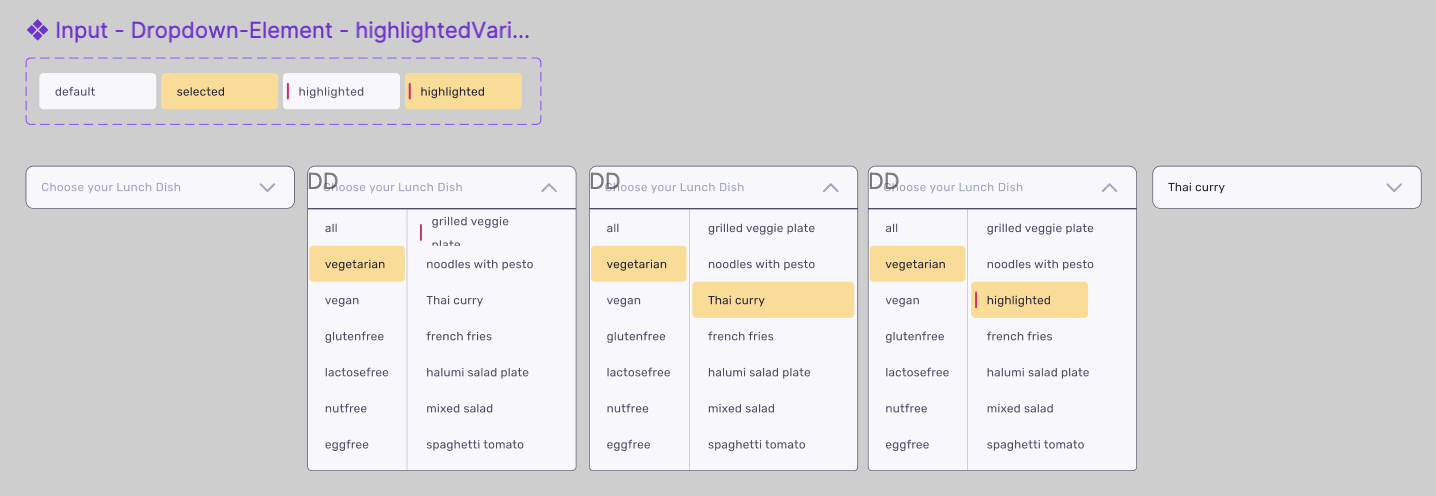
\includegraphics[width=100mm]{figma-prototype-1.png}
    \caption{Figma Prototyp - Dropdown Komponente 1}
    \label{img:figmaPrototype1}
\end{figure}

\begin{figure}[!htb]
    \centering
    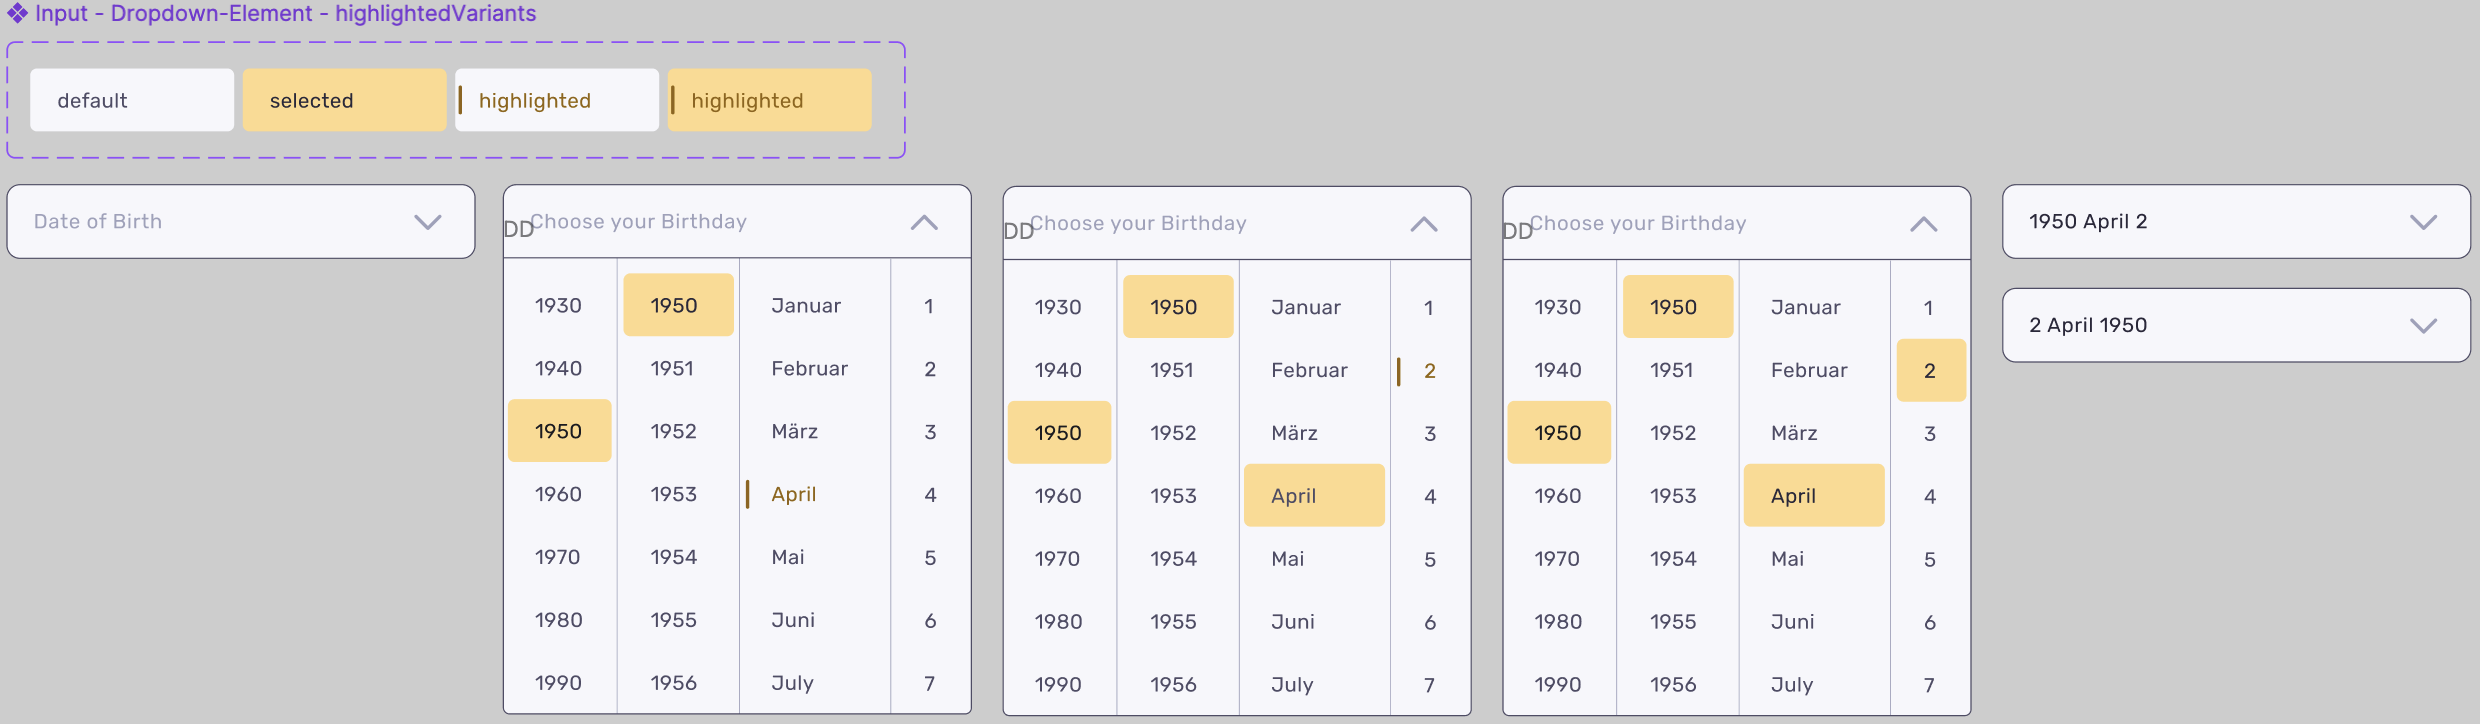
\includegraphics[width=100mm]{figma-prototype-2.png}
    \caption{Figma Prototyp - Dropdown Komponente 2}
    \label{img:figmaPrototype2}
\end{figure}

\begin{figure}[!htb]
    \centering
    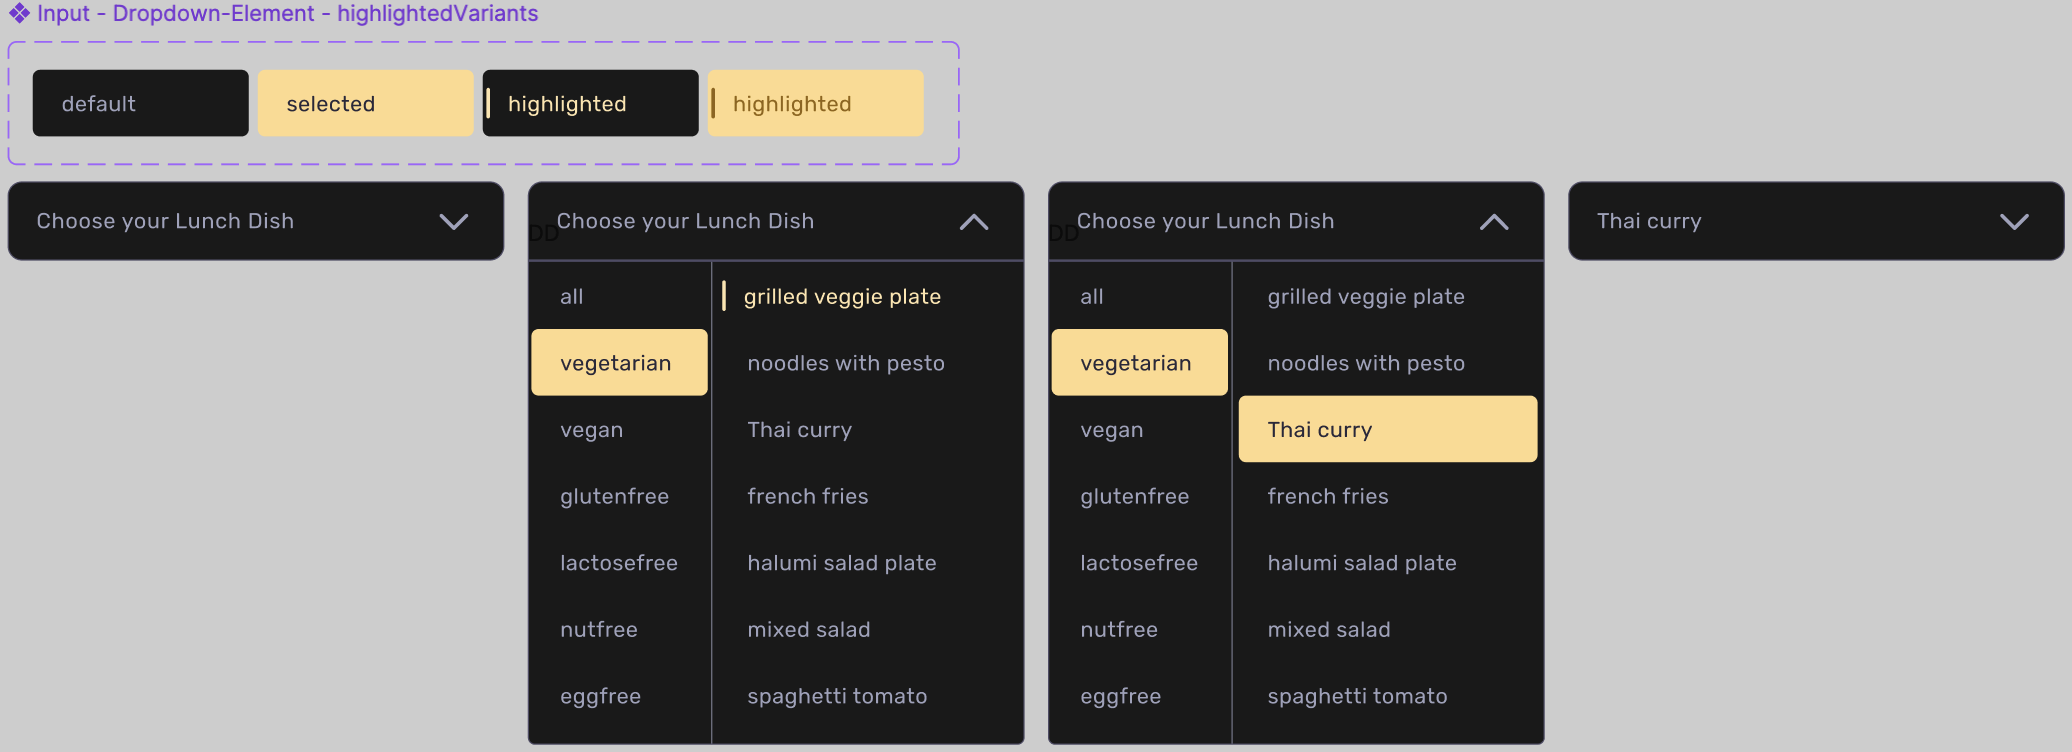
\includegraphics[width=100mm]{figma-prototype-3.png}
    \caption{Figma Prototyp - Dropdown Komponente 3}
    \label{img:figmaPrototype3}
\end{figure}


\subsection{Farbpalette und Kontrast}

Während das Kolibri-Designsystem eine Vielzahl von Farben bietet, wurden spezifische Anpassungen vorgenommen, um sicherzustellen, dass die Dropdown-Komponente gut lesbar ist. 
Um eine bessere Nutzerfreundlichkeit zu erhalten, gestaltet sich die Farbauswal (Abbildung \ref{img:designColors}) so, dass sie hohen Kontrast bietet und somit die Barrierefreiheit der Anwendung verbessert.

\begin{figure}[!htb]
    \centering
    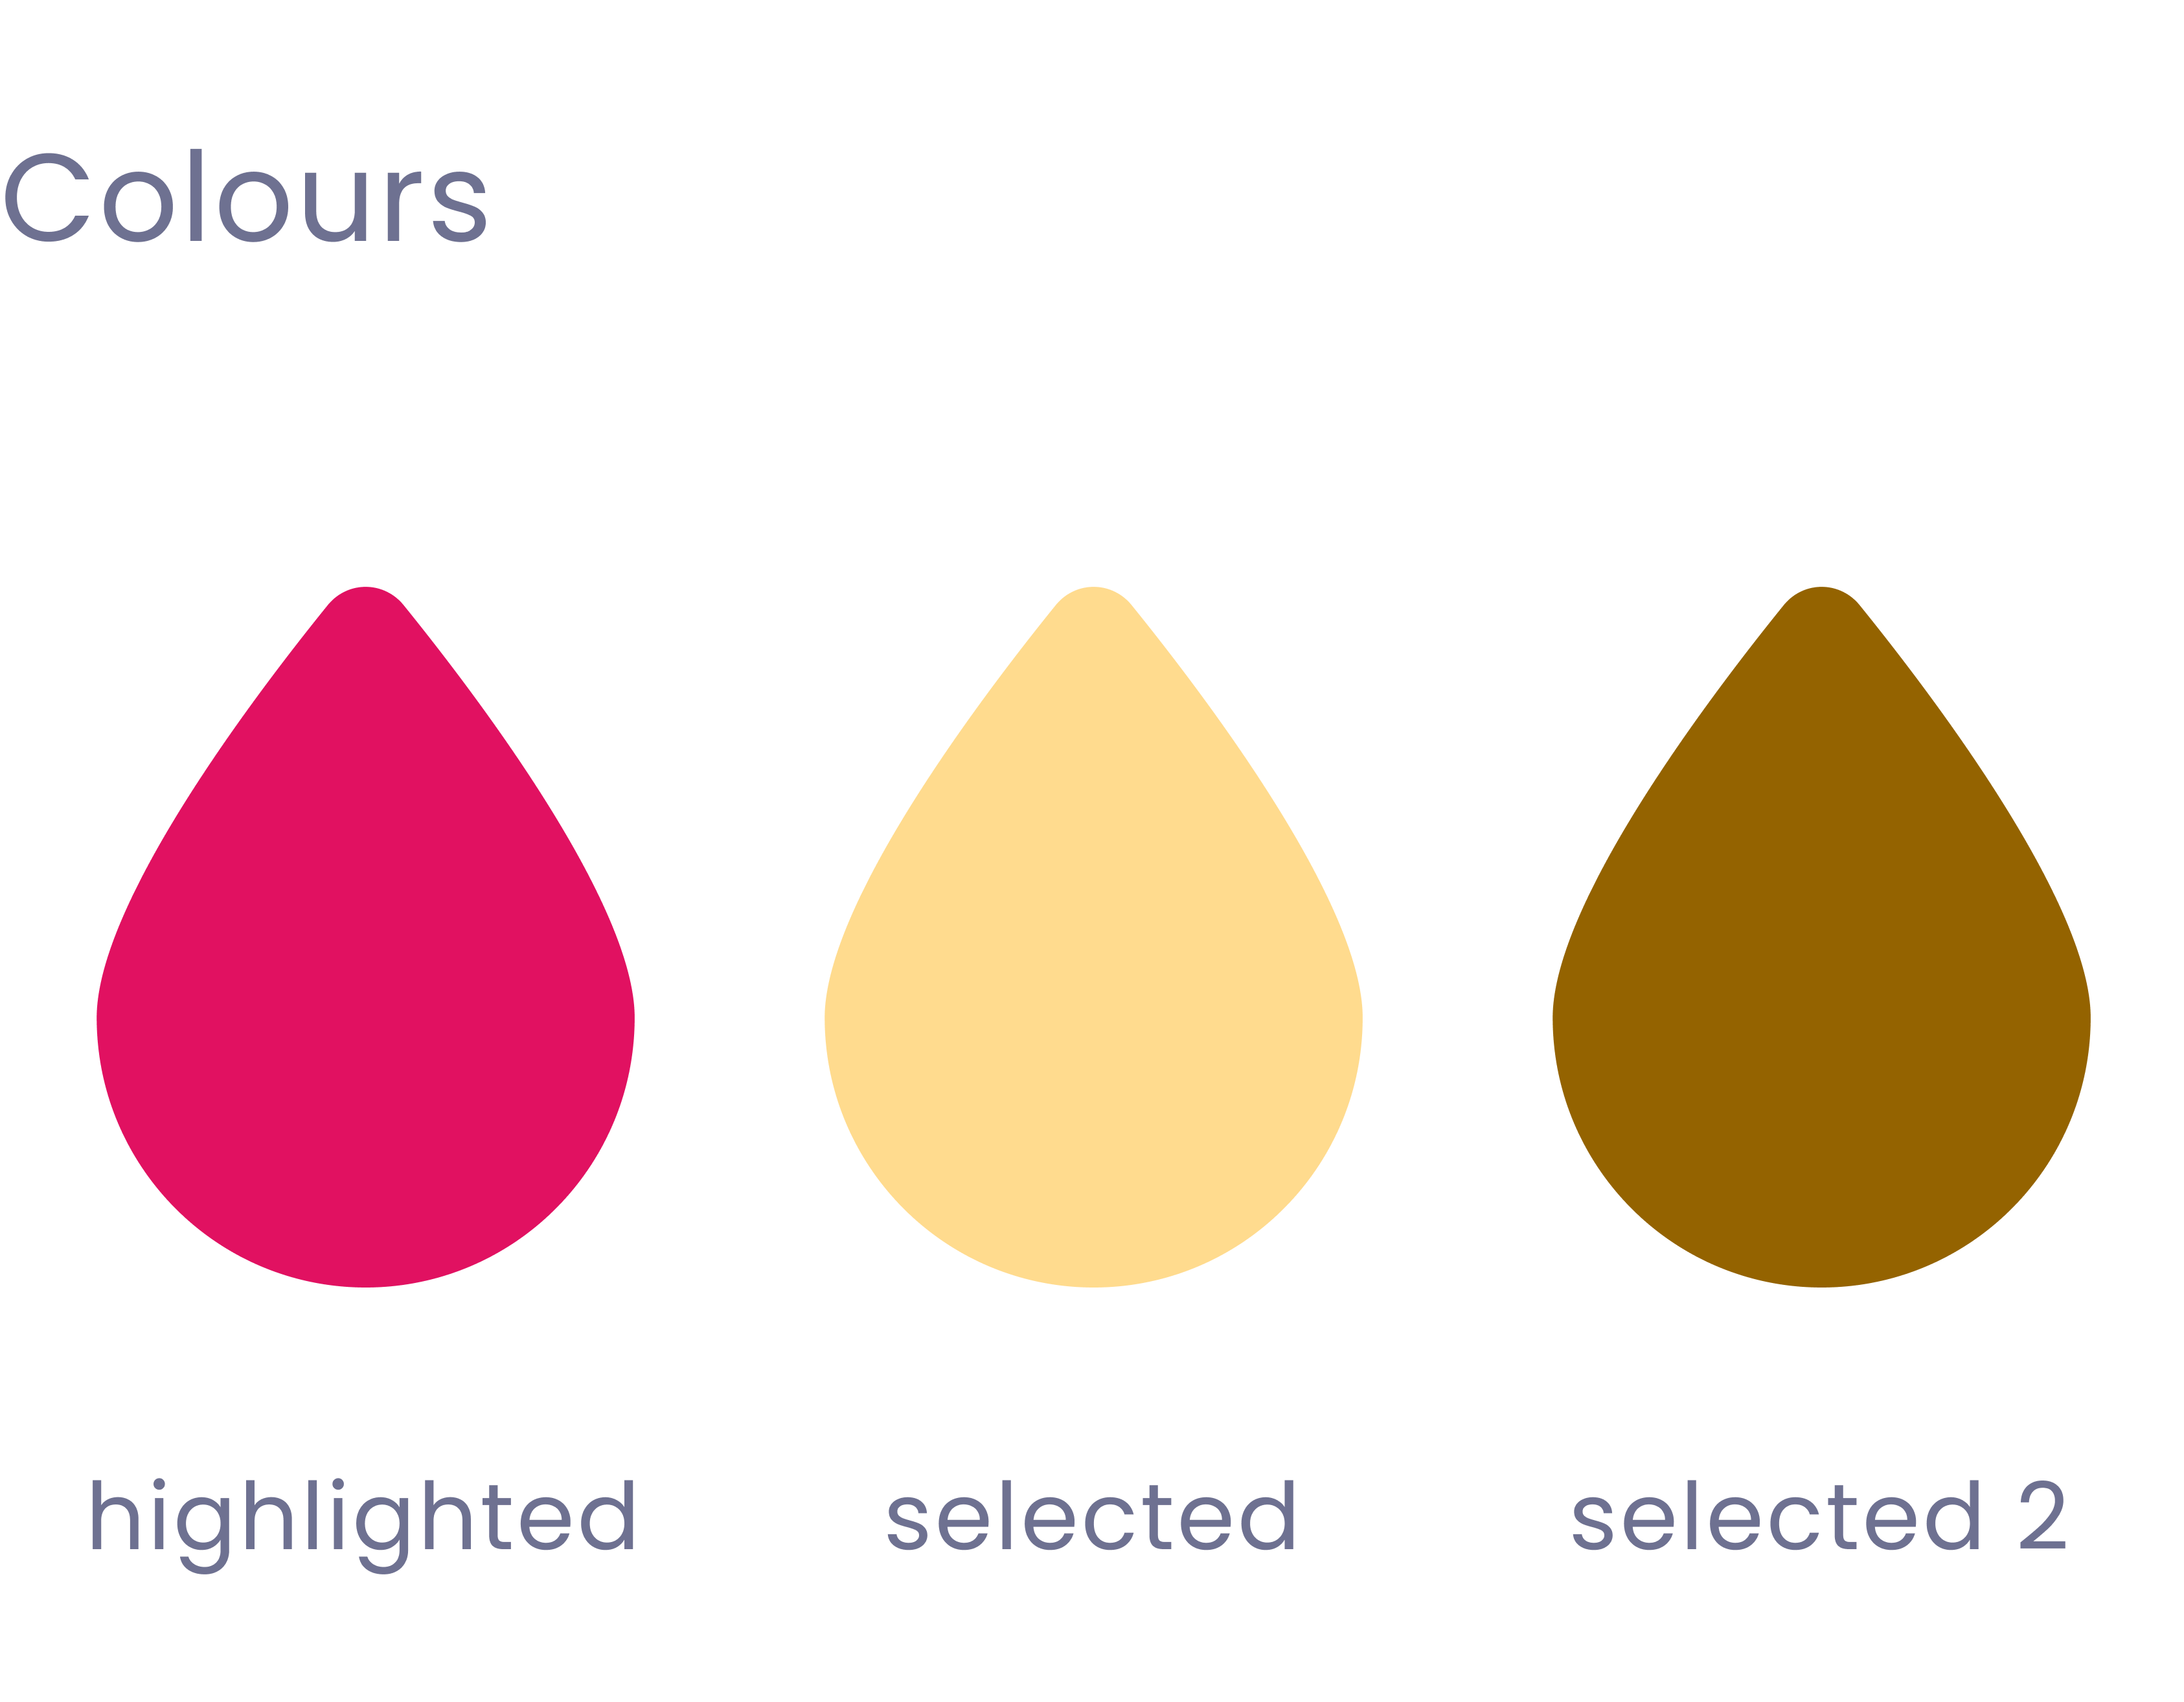
\includegraphics[width=70mm]{design-colors.png}
    \caption{Kolibri Design System - Farbpalette}
    \label{img:designColors}
\end{figure}

\noindent % todo originalen farben ?
Die originalen Farben erhalten im neuen Dropdown eine angepasst Verwendung:

\begin{itemize}
    \item \textbf{Original} $\rightarrow$ \textbf{Neu}
    \item Kolibri-Light/Yellow/300 $\rightarrow$ selected
    \item Kolibri-Light/Danger/--kb-danger-accent $\rightarrow$ highlighted
    \item Kolibri-Light/Warning/--kb-warning-dark $\rightarrow$ cursor position
\end{itemize}

\noindent
Der Code \ref{code:cssImports} zeigt die importierten CSS-Dateien, die als Grundlage für dieses Styling dienen:

\begin{lstlisting}[style = htmlcssjs, caption = CSS Imports, label = code:cssImports]
@import "../../../css/kolibri-base.css";
@import "../../../css/kolibri-light-colors.css";
\end{lstlisting}


\subsection{Layout und Typografie}

Um die in Figma entworfenen Designs umzusetzen, erhält die Dropdown-Komponente eigenes CSS.
Nachfolgend im Codeausschnitt \ref{code:styleDemoPage} ist der relevante CSS-Code, der zur Gestaltung der Dropdown-Komponente verwendet wird:
% todo code passt nicht zu text => code ist in selectprojector / columnoptionsprojetor jeweils unten
% todo reduzieren auf wesentliche stellen & beschreiben

\begin{lstlisting}[style = htmlcssjs, caption = style.css der Demo-Page, label = code:styleDemoPage]
body {
    perspective: 100vw;
}

.card {
    max-width:  40em;
    margin:     1em auto 2em auto;
    padding:    2em 4em;
    box-shadow: var(--kolibri-box-shadow);
    min-width:  620px;
}

h1 {
    text-align:  center;
    font-family: var(--font-sans-serif), sans-serif;
    margin-top:  0;
}

h3, h4 {
    margin-top: 3rem;
}

.holder {
    min-width: 160px;
    width: fit-content;
    margin: 1rem 0;
}

.holder > div {
    margin: 0;
    width: 100%;
}
\end{lstlisting}


\subsection{Interaktionsdesign}

Die Dropdown-Komponente ist so gestaltet, dass sie sowohl für Maus- als auch Tastaturbenutzer optimal funktioniert. 
Das Design der Interaktionen bietet eine intuitive und leicht zugängliche Bedienung der Komponente.
Um die Benutzerführung zu erleichtern, erhalten die hervorgehobenen (highlighted) bzw. ausgewählten (selected) Optionen eine Kennzeichnung durch spezifische CSS-Klassen.
Der CSS-Code \ref{code:styleExample} zeigt einen Style-Ausschnitt auf ein gehighlightetes Element.

% todo insert correct code in highlight
\begin{lstlisting}[style = htmlcssjs, caption = Style Beispiel für Zustand Highlight, label = code:styleExample]
.highlighted {
    background-color: #e0e0e0; 
}
\end{lstlisting}


\subsection{Komponentengrösse und Layoutanpassungen}

Mit der Definition von Mindest- und Maximalbreite sowie flexiblen Layouts ist sichergestellt, 
dass die Dropdown-Komponente auf verschiedenen Bildschirmgrössen funktioniert und sich gut darstellen lässt.

% todo code wieder für demo und nicht komponte => ändern & beschreiben
\begin{lstlisting}[style = htmlcssjs, caption = Flexible Layouts für Demo-Page, label = code:layoutDemoPage]
#componentCity .select-input-component {
    min-width:  400px;
}

#componentImg .select-input-component,
#componentCountry .select-input-component {
    min-width:  320px;
}

#componentImg .options-column {
    width: auto;
}

#componentImg img {
    width:  2rem;
    max-height: 1.3rem;
    object-fit: contain;
}

form {
    display: flex;
    gap: 2rem;

    > button {
        border-radius: 5px;
        color: white;
        background-color: var(--kolibri-color-output);
        font-weight: bold;
        outline: none;
        border: none;
        padding: .5rem;

        &:focus {
            filter: brightness(150%);
        }
    }
}

label {
    display: flex;
    align-items: center;
}
\end{lstlisting}


\subsection{Benutzerfeedback und Prototyping}

Der Einsatz von interaktiven Figma-Prototypen ist hilfreich beim Evaluieren der initialen Benutzerfreundlichkeit und intuitiven Bedienung. 
Mit der Integration der Rückmeldungen von Benutzerinteraktionen in das Design verbessert sich die Usability kontinuierlich.
Beispiele für die Prototypen und verschiedene Zustände der Dropdown-Komponente ist im oberen Hälfte des Bildes \ref{img:figmaPrototype1} ersichtlich.

Die Gestaltung der Auswahlkomponente umfasst sowohl visuelle als auch funktionale Aspekte. 
Gezielte CSS-Anpassungen und ein durchdachtes Interaktionsdesign finden in der Realisierung ihren Platz. 
Das Ziel ist, eine ansprechende und benutzerfreundliche Komponente zu schaffen. 
Sie fügt sich nahtlos in das Kolibri-Designsystem ein und überzeugt gleichzeitig durch optimierte Les- und Bedienbarkeit.


\section{Interaktionen}

Damit ein gemeinsames Verständis entsteht, gilt es für die Bedienung der Komponente Regeln festzulegen.
Wie in den Grundlagen bereits beschrieben kann sich ein Wert aus dem Optionen-Container in verschiedenen Zuständen befinden.
In diesem Absatz spielen Selektion, Highlight und Cursor Position eine Rolle.
Zur Auffrischung: 

\begin{itemize}
    \item \textbf{Selektion}: Ausgewählter Wert der Spalte
    \item \textbf{Highlight}: Element unterhalb des Mauszeigers
    \item \textbf{Cursor Position}: Position (Element) der Tastatur
\end{itemize}

\noindent
Bei der Festlegung der Maus-Interaktion fiel die Entscheidung auf folgendes:

\begin{itemize}
    \item \textbf{mouseover}: visuelles Highlighting des Elements ohne Selektionsänderung
    \item \textbf{click}: Änderung der Cursor Position \& direkte Selektionsänderung
\end{itemize}

\noindent
Die Tastatur-Steuerung mit den Pfeiltasten hingegen hält sich an diese Bedienungen:

\begin{itemize}
    \item Änderung der Cursor Position
    \item \textbf{selbe Spalte}: direkte Selektionsänderung ohne weitere Bestätigung
    \item \textbf{Spaltenänderung}: keine Selektionsänderung
\end{itemize}

\noindent
Anhand dieser Regeln entstanden folgende Aktionen als Basis für den ersten Projektor der neuen Komponente. 


\clearpage
\import{../tables}{d.newComponent.tex}

Das Undo und das Redo auf der Komponente erhält im ersten Projektor keine spezielle Definition.
Gewisse Verhaltensweisen finden sich im geschlossenen als auch offenen Zustand der Komponente wieder.
Anders als bei den existierenden Komponenten, ist bei der Neuen die Leertaste neu belegt. 
Ist die Liste bereits offen, wird der sich aktuell unter der Cursor Position befindliche Wert selektiert.
Die Interaktionen können in weiteren Projektoren angepasst bzw. geändert werden.


\section{Prinzipien \& Regeln}

Um stabilen und verständlichen Code zu garantieren, hält sich dieses Projekt an diverse Prinzipien.
Ein Ansatz ist alle Objekte so immutable als möglich zu halten.
Dadurch können unerwartete Änderungen vermieden werden.
Weiter gilt es, die Bestandteile im KISS-Stil umzusetzen.
Dazu zählt, dass die einzelnen Objekte und Funktionen möglichst privat zu gestalten sind.
Die Bausteine sind kurz und übersichtlich aufzubauen.
Zu diesem Zweck soll Separation of Concern eingesetzt werden, so dass jede Funktion nur eine Aufgabe zu erfüllen hat.
Damit der Code einfach und lesbar bleibt bzw. wird, gilt es, Entscheidungen zu treffen.
Zu diesen Entschlüssen zählt das bewusste Weglassen von Funktionalität und somit auch Komplexität.

Beim implementieren ist darauf zu achten, den Code sauber zu formatieren.
Zudem ist es sinnvoll, die Änderungen regelmässig mit dem Code-Analyse-Tool von Intellij auf ihre Qualität zu prüfen. 
Diese Prinzipien und Regeln unterstützen eine ordentliche Entwicklungsumgebung für eine stabile Komponente.
Das Kapitel Patterns bietet eine weitere Möglichkeit den Code strukturiert zu halten.


\section{Patterns}

In diesem Projekt finden sich einige Code-Patterns wieder.
Die Wichtigesten wie Null-Object, Projector und Decorator sind in den nachfolgenden Unterkapitel genauer erläutert.
Eine weitere Rolle spielt unter anderem die Master-Detail-View, aber im Zusammenhang mit der Komponente eher nebensächlich.
Zudem ist die Anwendung nicht typisch bzw. genau abgegrenzt.
Die Implementation erhält durch die verwendeten Patterns eine Struktur und läuft stabiler.


\subsection{Null Object Pattern}

Ein Pattern, welches im Verlauf der Arbeit eine wichtige Rolle eingenommen hat, ist das Null-Object Pattern.
(\cite{nullObjectPattern}) Null hat den Nachteil, dass alle Funktionsaufrufe darauf zu Fehlern führen.
Das Null-Object besteht aus vordefinierten Default-Werten und besitzt Do-Nothing-Implementationen für alle Funktionen.
Durch die Verwendung dieses speziellen Objekts entfällt eine ansonsten notwendige Nullwertprüfung.
Zudem ist jedes erstellte Null-Object wertegleich.

Um eine Selektion zurücksetzen zu können, muss diese Komponente eine Null-Option enthalten.
Die Verwendung des Null-Objects findet sich an mehreren Stellen des Codes wieder.
Die Definition der angewendeten Null-Option zeigt der nachfolgende Code.

\begin{lstlisting}[style = htmlcssjs, caption = Null-Option, label = code:nullOption]
/** @private @returns { OptionType } */
const reset = () => {
    return Option(null, null);
};

/** @public @type { OptionType } */
const nullOption = reset();
\end{lstlisting}

Hierbei muss nur die $nullOption$ selbst exportiert werden und das Reset bleibt $private$.
Um die selbe Funktionalität wie die gewünschten Objekte zu bieten, erhält diese Konstante den Typ $Option$.
Der Codeausschnitt \ref{code:nullOption} befindet sich in der Datei $optionsModel.js$.
Mehr zur File Aufteilung ist in den nächsten zwei Unterkapiteln zu lesen.

\subsection{Projector Pattern}

(\cite{projectorPattern}) Das Projector Pattern basiert auf dem verbreiteten Model-View-Controll Pattern.
Das Model verwaltet die Daten, welche dargestellt werden sollen.
Zudem enthält die Komponente des Patterns die Geschäftslogik und verarbeitet die Regeln und Anfragen für die Daten.
Ein Controller generiert privat gehaltene Modelle.
Dabei werden nur die notwendigen Funktionen zur Verfügung gestellt.
Diese Funktionen können Getter, Setter und Listener der observierten Modelle und Werte sein.
Der Projektor bindet Daten-Modelle über den Controller an die View.
Auf der anderen Seite wird die View an die Models gebunden, dies erneut durch die Verwendung des Controllers.
Aus den Bindings und den Daten generiert ein Projetor die passende View.
Die View ist passiv und hat keine Kenntnis über die anderen Komponenten.

Dieses Pattern zeigte sich als eines der Wichtigsten für die Erstellung der neuen Komponente.
In den folgenden Grafiken sind Models als Zylinder, Controller als schiefes Rechteck und Projectors als Oval dargestellt.
Die Raute mit Option ist ein Daten-Typ, der über das gesamte Projekt seine Anwendung findet.
Das $starter.js$ beinhaltet alle Bestandteile, welche für eine Anwendung benötigt werden.
Das Puzzle wird im späteren Unterkapitel Decorator Pattern genauer beschrieben.
Die erste Implementation, welche dieses Pattern verwendet, ist auf Abbildung \ref{img:DiagramSelectComponentOld}.

\begin{figure}[!htb]
    \centering
    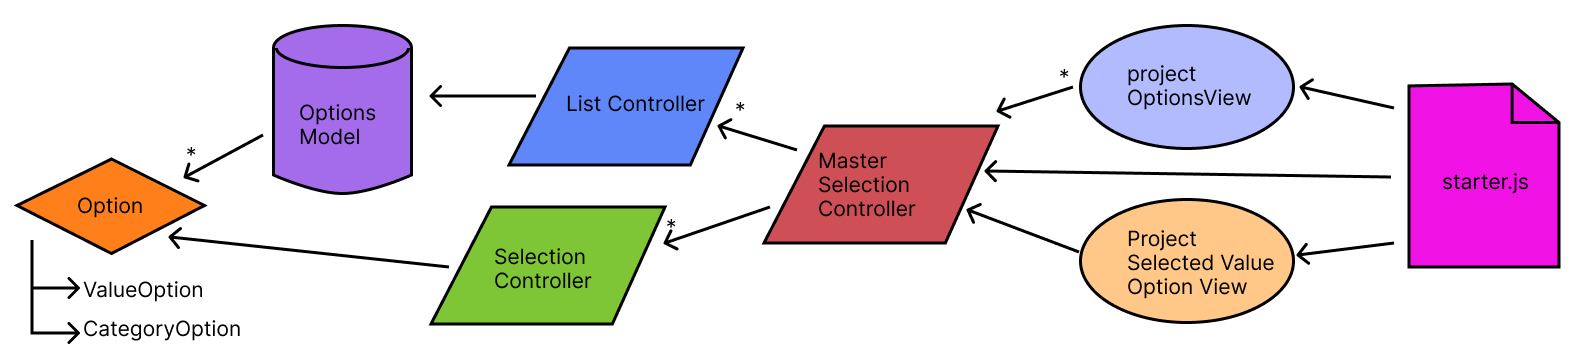
\includegraphics[width=120mm]{diagram-select-component-old.png}
    \caption{Diagramm Select Component - 1. Version}
    \label{img:DiagramSelectComponentOld}
\end{figure}

Diese Version zeigt noch viel Komplexität und duplizierenden Code in den einzelnen Funktionen.
Eine genaue Analyse der Komponente zeigt, dass sich das Pattern zwei Mal anwenden lässt.
Die neue Aufteilung ergibt die zwei folgenden Abbildungen \ref{img:DiagramColumnComponent} und \ref{img:DiagramSelectComponent}.
Die Implementation der dargestellten Diagramme resultiert aus einem Refactoring im grösseren Rahmen.

\begin{figure}[!htb]
    \centering
    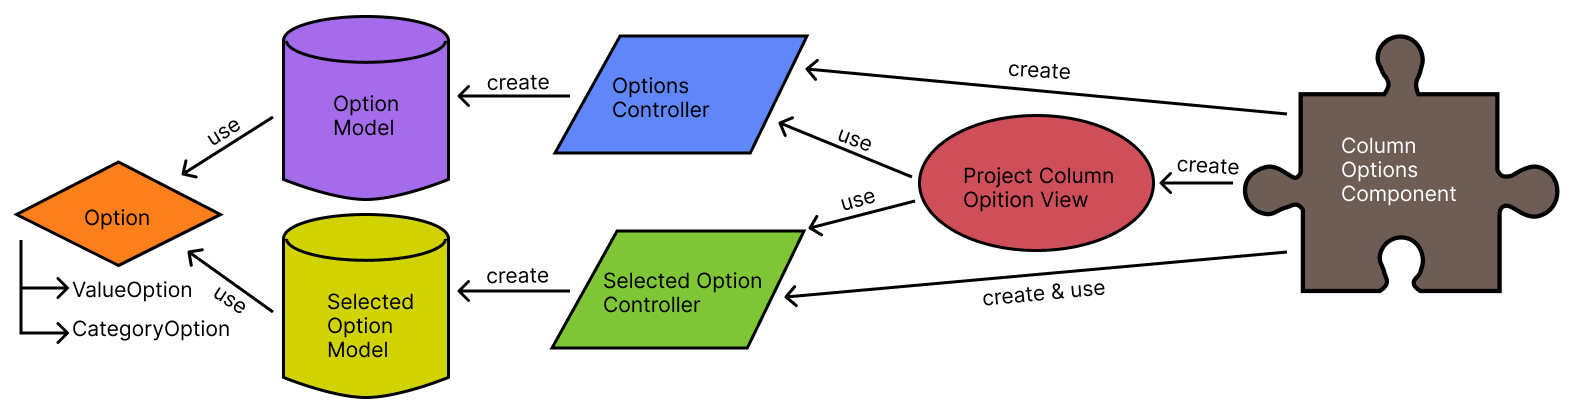
\includegraphics[width=120mm]{diagram-column-component-with-desc.png}
    \caption{Diagramm Column Component}
    \label{img:DiagramColumnComponent}
\end{figure}

Zum einen findet sich das Projector Pattern in einer einzelnen Spalte in der Options-Liste wieder.
Pro Kolonne existiert eine Auswahl und eine Menge von Optionen.
Diese beiden Bestandteile besitzen je ein eigenes Model und einen eigenen Controller.
In diesem Fall generiert der Projektor eine gemeinsame View mit Bindings zu den beiden Controllern.
Bei einer Anwendung übernimmt die $ColumnComponent$ die Verwaltung gewisser Bausteine (Mehr dazu später).

\begin{figure}[!htb]
    \centering
    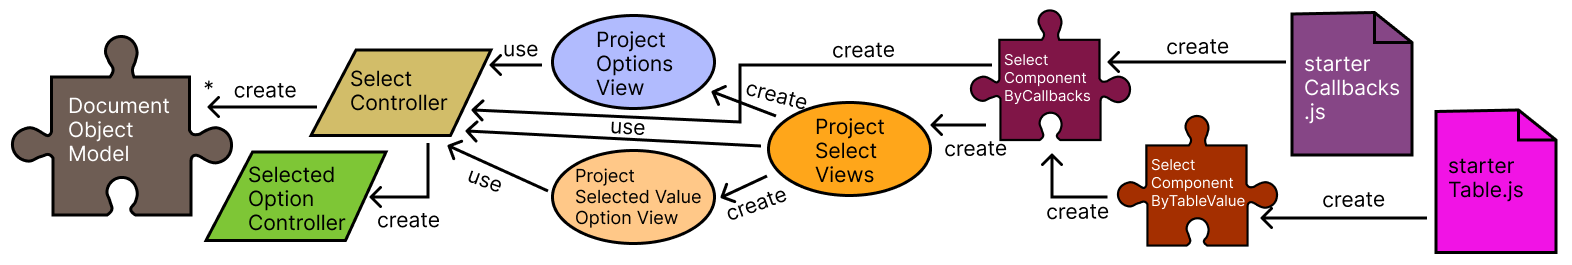
\includegraphics[width=120mm]{diagram-select-component-with-desc.png}
    \caption{Diagramm Select Component}
    \label{img:DiagramSelectComponent}
\end{figure}

Die Anwendungskomponente einer Column findet sich als Bestandteil des zweiten Projector Pattern wieder.
Ein $SelectController$ verwaltet eine bis mehrere $ColumnComponent$s als auch ein Element für die Tastaturnavigation.
Die sogenannte Cursor Position verwendet im Hintergrund ebenfalls einen $SelectedOptionController$. 
Dieser ist der selbe wie in der Abbildung \ref{img:DiagramColumnComponent} und findet hier eine Wiederverwendung.
Um die Bindings zu definieren, greifen die einzelnen Projektoren auf den selben Controller zu.
Der Master-Detail-Aufbau der neuen Komponente findet sich in der Aufteilung der Projektoren wieder.
Der Detail-Baustein kümmert sich um die aktuelle Auswahl und das Eingabefeld.
Die Master-Komponente verwaltet alle Spalten mit den Kategorie- und Werte-Optionen, sowie dessen Bindings.
In einer weiteren Funktion werden die beiden Projektoren zusammengeführt und in eine gemeinsame View eingebettet.
Auch diese Projector Pattern Anwendung schliesst mit einer Component - der SelectComponent - ab.
Mehr zu dieser und der Column-Component steht im nächsten Kapitel.


\subsection{Decorator Pattern}

(\cite{decoratorPattern}) Ein Decorator bietet zusätzliches Verhalten ohne das Originale Objekt zu verändern.
Zudem können verschiedene Funktionen kombiniert werden.
Dieses Pattern ermöglicht die Erstellung eines modularen und anpassbaren Codes.
In diesem Projekt unterstützt es die Gestaltung und Erweiterung der Auswahlkomponente.

Wie im vorherigen Kapitel erwähnt, besteht die neue Komponente unter anderem aus zwei sogenannten Component-Bausteinen.
Die Decorator sind in den Abbildungen \ref{img:DiagramColumnComponent} und \ref{img:DiagramSelectComponent} als Puzzle dargestellt.
Diese Bestandteile kombinieren die Funktionalität des Controllers mit der Erstellung der View.
Dadurch lässt sich die neue Komponente einfacher anwenden.

\begin{lstlisting}[style = htmlcssjs, caption = SelectComponentByTableValue dekoriert SelectComponentByCallback, label = code:componentDecorator]
const SelectComponentByTableValues = (
    selectAttributes,
    optionsTable,
    sortColumnOptionsAlphabetical = false
) => {
    /* code for mapping between table and callbacks */
    const component = SelectComponentByCallbacks(selectAttributes, callbacks);
    return {
        ...component,
    };
};
\end{lstlisting}

Ein weiterer Einsatzort ist bereits in der Abbildung \ref{img:DiagramSelectComponent} aus dem Vorkapitel zu erahnen.
Der rotbraune $SelectComponentByTableValue$ in Code \ref{code:componentDecorator} dekoriert die $SelectComponentByCallback$.
Damit bietet die neue Komponente zwei verschiedene Möglichkeiten der Anwendung.
Das nächste Kapitel geht genauer auf den Master-View-Bereich des $SelectProjector$s - Abbildung \ref{img:DiagramSelectComponent} - ein.


\section{Dropdown-Container}

Um alle Optionen zu gegebener Zeit darzustellen, stehen verschiedene Varianten zur Auswahl.
Eine Möglichkeit ist, den Container als HTML-Dialog zu gestalten.
Die vorhandenen Funktionen sind jedoch nicht für diese Komponente geeignet.
Für den gewünschten Zweck erfordert das Dialog-Element noch einiges an benutzerdefinierter Anpassung.

Eine weitere Variante ist, ein normales $div$ als Options-Container zu verwenden.
Dies erfordert ebenfalls einen enormen Implementationsaufwand.
Eine Andwendung dieses Ansatzes findet sich in der ersten Version der Komponente.
Hierbei eröffnet sich das Problem von der Inkonsistenz zwischen UI und Controller.
Zudem ist es möglich, dass unerwünscht mehrere Dropdown-Container gleichzeitig offen sind.

Als dritte Möglichkeit bietet sich die Popover-API an, welche seit 2024 von allen gängigen Browser unterstützt wird.
Durch das Refactoring der Variante mit dem normalen Div-Container resultiert eine Version mit der Anwendung dieser API.
Der Zusatzaufwand reduziert sich im Gegensatz zu den beiden oben erwähnten Container-Implementationen.
Der Grundaufbau des Popover-Container ist im folgenden Code \ref{code:PopoverExample} dargestellt.

\begin{lstlisting}[style = htmlcssjs, caption = Popover-Container Beispiel, label = code:PopoverExample]
<div popover="auto"
    id="select-component-0-options" 
    class="options-component" 
> </div>
\end{lstlisting}

Bei diesem Codeausschnitt ist wichtig, dass das Attribut $popover$ den Wert $auto$ erhält.
Dies bewirkt, dass die Popover sich automatisch schliessen, wenn ein Klick ausserhalb des Container passiert.
Das Öffnen und Schliessen des Dropdown-Elements kann über das $popovertarget$-Attribut mit der Popover-Id\footnotemark auf der Bedienkomponente gesteuert werden.
\footnotetext{$id$-Attribut des Div-Containers mit dem Attribut $popover$}
Als Alternative dazu besteht die Möglichkeit, das Popover über JavaScript zu steuern.
Hierbei besteht die Möglichkeit auf den Status und das Event des Togglens zuzugreifen.
Diese Funktionalitäten erlauben den Controller konsistent zum UI zu halten.


\section{Performance}

Um eine gute Performance zu bieten, ist es notwendig den Aufbau-Prozess einer Webseite zu kennen.
Dieser Ablauf ist im Kapitel \textbf{Grundalgen} unter \textbf{Ablauf Parsing \& Rendering} genau beschrieben.
Die folgende Abbildung \ref{img:RenderingProcessRecap} zeigt den Prozess im Überblick.

\begin{figure}[!htb]
    \centering
    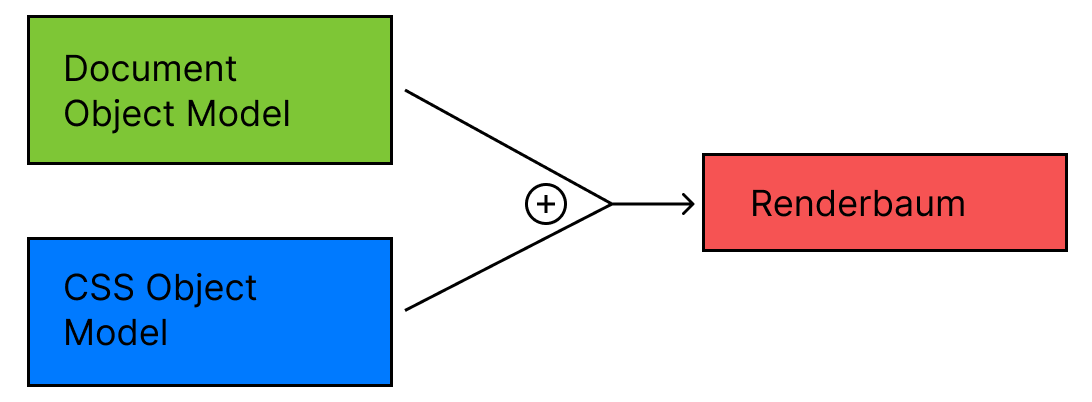
\includegraphics[width=120mm]{rendering-process.png}
    \caption{Rendering Prozess}
    \label{img:RenderingProcessRecap}
\end{figure}

Hierbei ist ein wichtiger Punkt, dass der Browser den Renderbaum (in der Abbildung \ref{img:RenderingProcessRecap} rot) maximal 60 Mal pro Sekunde neu zeichnen kann.
Daher müssen viele kleine Änderungen ausserhalb des Renderbaums - am besten in einem sogenannten Shadow-DOM - geschehen.
Ein Shadow-DOM ist ein Teilbaum, welcher nicht im Renderbaum angehängt ist.
Um dies zu bewerkstelligen, ist es sinnvoll, die Änderungen nach dem Abhängen des Elternknotens zu vollziehen. 
Nach den Änderungen kann der Teilbaum wieder an den gewünschten Ort platziert werden.

\begin{lstlisting}[style = htmlcssjs, caption = Performance Optimierung (columnOptionsComponent.js), label = code:PerformanceOptimization]
const addAllOptions = (options) => {
    const placeHolder = createHolder();
    columnView.replaceWith(placeHolder);
    if (options.length > 50) {
        setTimeout(() => {
            options.forEach((option) => {
                optionsController.addOption(option);
            });
            updateScrollbar(columnView);
            placeHolder.replaceWith(columnView);
        }, 80);
    } else {
        options.forEach((option) => {
            optionsController.addOption(option);
        });
        updateScrollbar(columnView);
        placeHolder.replaceWith(columnView);
    }
};
\end{lstlisting}

Code \ref{code:PerformanceOptimization} ist eine Stelle, die diese Technik verwendet.
Hier wird ein Platzhalter mit einem Lade-Indikator an die Ursprungsstelle gesetzt, damit der Nutzer ein Feedback erhält.
Sobald der SpaltenContainer abgekoppelt ist, lädt die Funktion die Optionen in den Shadow-DOM.
Nach Abschluss wird der Container mit den neuen Elementen an die originale Stelle zurückersetzt.

(\cite{efficientDomManipulation}) Weiter ist darauf achten, dass CSS-Klassen an Stelle von Inline-Styles verwendet werden sollten.
Das Cachen von mehrfach verwendeten Selektoren verbessert die Effizienz des DOMs.
Die Selektoren sollten hierarchisch möglichst flach und nicht verschachtelt sein.
Wenn es die Situation erlaubt, ist es besser, nicht mit $innerHTML$ zu arbeiten.
In diesem Projekt ist es für die Anzeige der Label jedoch nötig $innerHTML$ zu nutzen.
Dies liegt daran, dass ein Label auch ein Bild enthalten kann.
Generell verwendet die neue Auswahlkomponente keine Inline-Styles.
Die einzigen Ausnahme betrifft das verborgene Eingabefeld. 
Durch den Code \ref{code:InlineStyle} sind die Properties vor dem Überschreiben geschützt.

\begin{lstlisting}[style = htmlcssjs, caption = Inline-Style für Inputfeld, label = code:InlineStyle]
inputElement.setAttribute(
    "style", "all: unset !important; z-index: -1 !important; " +
    "position: absolute !important; inset: 5px !important; " +
    "color: transparent !important; pointer-events: none !important;"
);
\end{lstlisting}

Die Regeln in Code \ref{code:InlineStyle} sorgen dafür, dass das Input-Feld transparent als auch resetet ist.
Zudem befindet es sich im Hintergrund und besitzt dieselben Grösse wie der Container mit dem ausgewählten Wert.

\subsubsection{\color{dgray} Performance Vergleich}

Durch die Anpassungen der Performance Optimierung, verbesserte sich die Ladezeit bei grossen Datenmenge enorm.
Die Testseite enthält vier existierende und vier neue Auswahlkomponenten mit den selben Inhalten wie je eines der Existierenden.
Je eine der Selects enthält eine grosse Datenmenge von über 4'000 Werten.
Die folgenden zwei Bilder \ref{img:PerformanceTestBefore} und \ref{img:PerformanceTestAfter} zeigen die Messung während des Seitenaufbaus.

\begin{figure}[!htb]
    \centering
    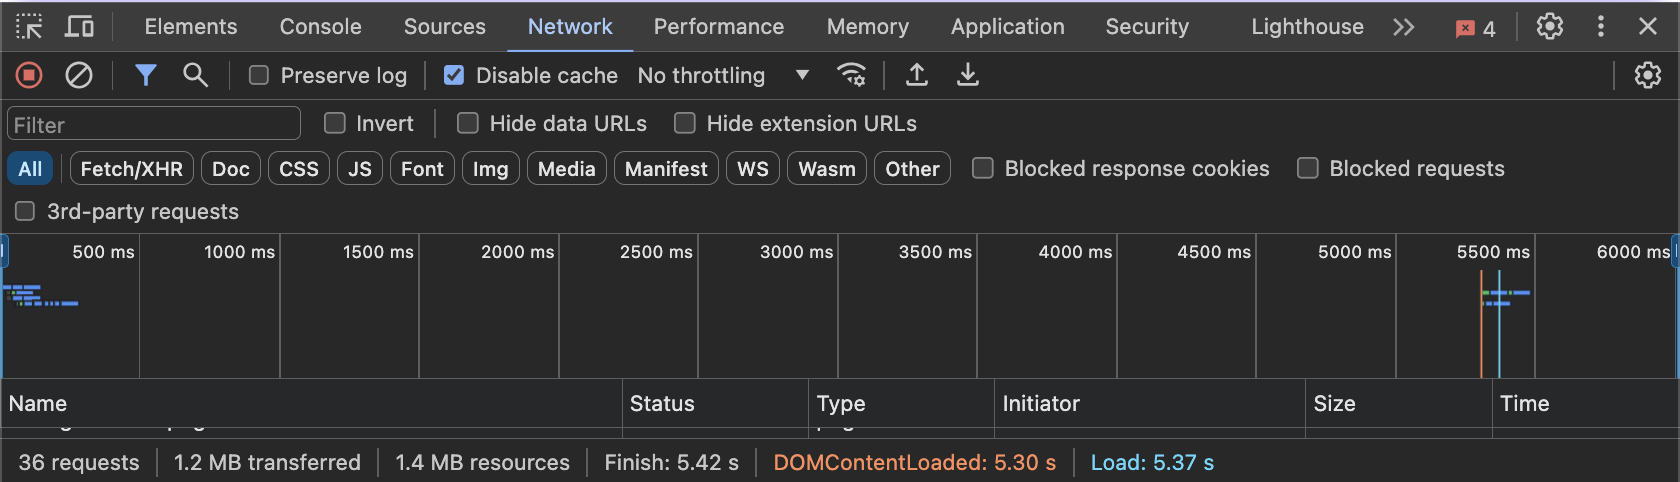
\includegraphics[width=100mm]{performance-before-user-tests.png}
    \caption{Performance Test vor Anpassungen}
    \label{img:PerformanceTestBefore}
\end{figure}

Auf der Grafik \ref{img:PerformanceTestBefore} ist zu sehen, dass der Seitenaufbau der früheren Version sehr lange dauerte.
Dies bestätigen mehrere Feedbacks der Nutzer, später mehr dazu.

\begin{figure}[!htb]
    \centering
    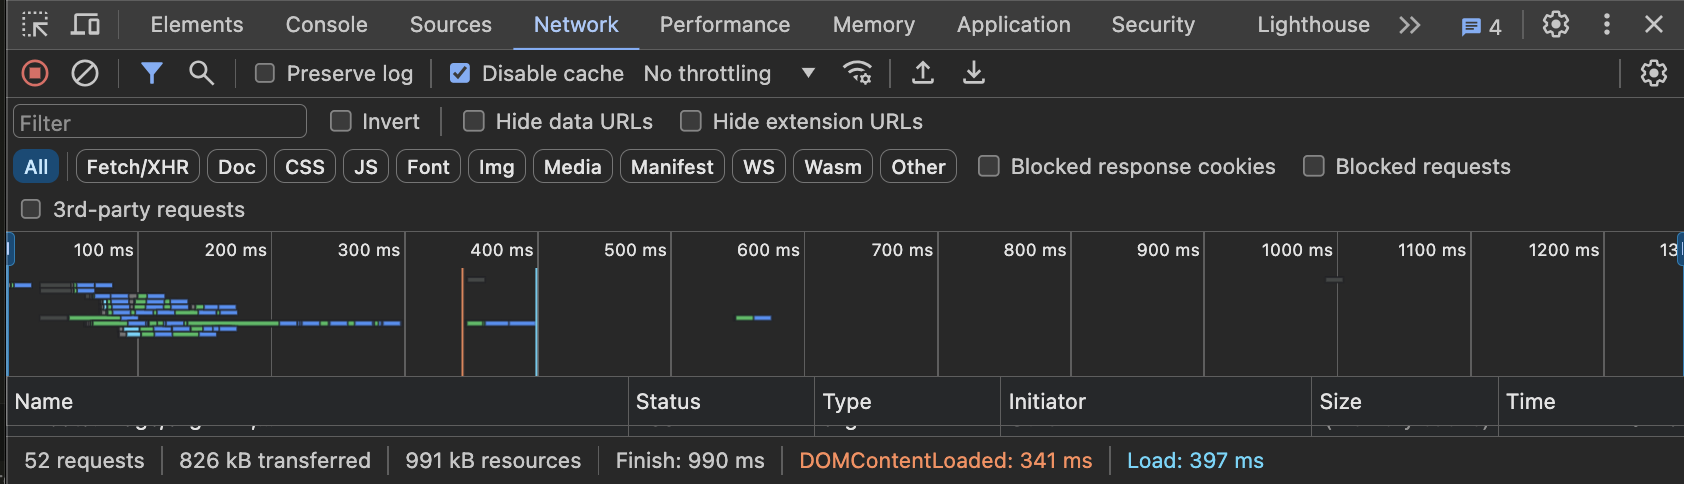
\includegraphics[width=100mm]{performance-after-user-tests.png}
    \caption{Performance Test nach Anpassungen}
    \label{img:PerformanceTestAfter}
\end{figure}

Der Vergleich zwischen Abbildung \ref{img:PerformanceTestBefore} und \ref{img:PerformanceTestAfter} zeigt, dass die Seite um einen Faktor 13 besser ist.
Die oberen Grafik zeigt die Messung der Implementation, welche sehr viele Aktionen auf dem Renderbaum ausführt.
Ein Refactoring führt zur Verschiebung dieser Arbeiten auf den Shadow-DOM.
Dadurch verkürzt sich der Ladevorgang um vier bis fünf Sekunden.
Feedbacks zu den durchgeführten User-Tests mit Programmierern als auch Endnutzern sind im nachfolgenden Kapitel aufgeführt.


\section{Testing}

\subsection{Automated Tests}

% todo text for tests
\begin{figure}[!htb]
    \centering
    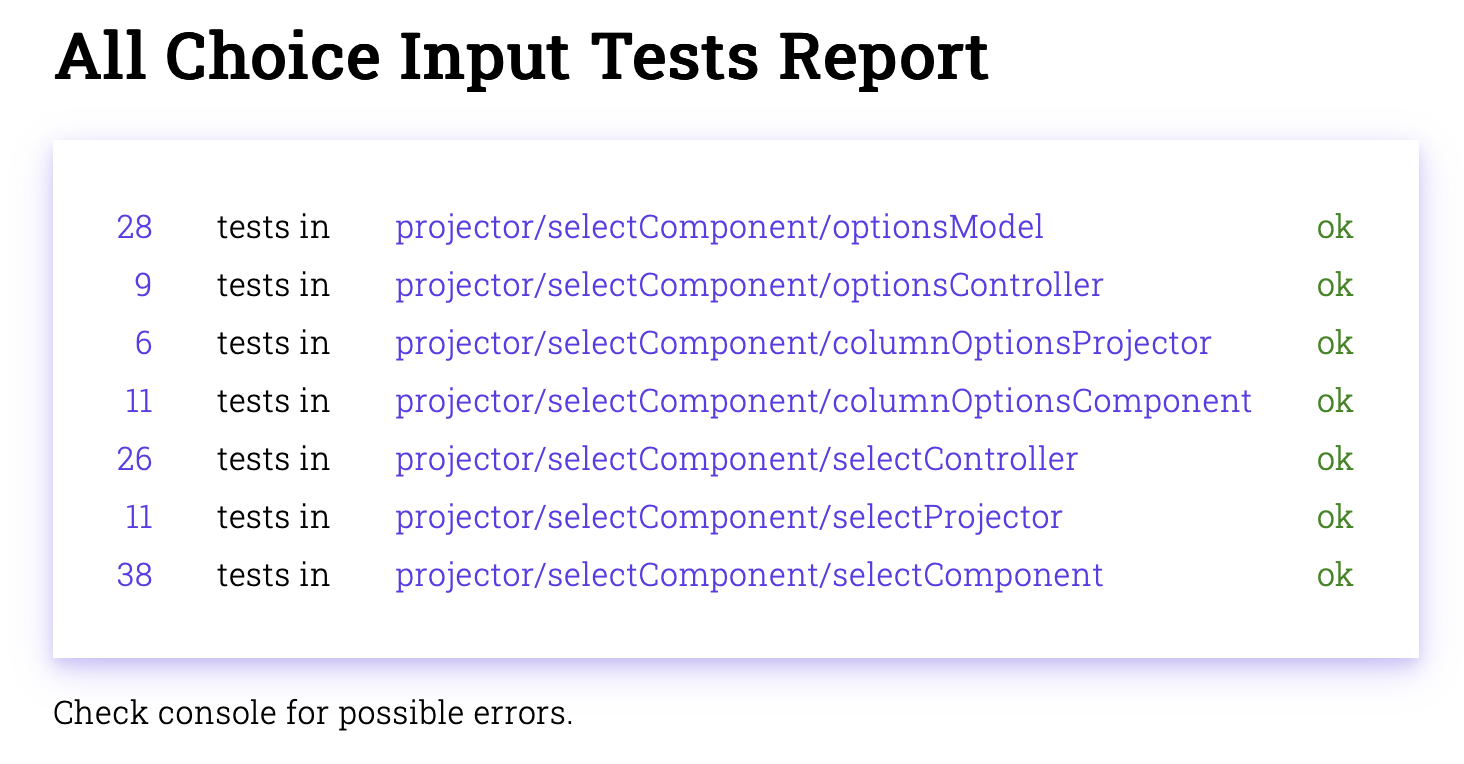
\includegraphics[width=100mm]{automatedTests.png}
    \caption{Automatisierte Tests}
    \label{img:automatedTests}
\end{figure}

\subsection{User Tests} % todo

% personas im anhang

\subsubsection{Programmierer}

% images und text von umfrage im anhang

\subsubsection{Formular-Ausfüller}



\section{Diskussion}

% herausforderungen
% komplexeste probleme
% erfolge
% unerwartete wendungen
% entscheidungen, gründe => kein filter/ suche

\section{Fazit}

\chapter{Diskussion}
\label{chap:discussion}

Die in Kapitel \textbf{\ref{chap:existingComponents}} beschriebenen Komponenten Select und Datalist kommen in vielen Webseiten zu Anwendung. 
Das Auswählen eines Wertes aus einer vorgegebenen Menge ist mit diesen Elementen ineffizent und unästhetisch. 
Die in Projekt 5 erstellte Länderauswahl löst das Problem aber nur für diesen einen spezifischen Anwendungsfall. 
Die neue Komponente \codestyle{SelectComponent} baut auf der Länderauswahl auf, ist jedoch generalisiert und lässt sich mit unterschiedlichsten Werten anwenden. 
Dabei spielt es keine Rolle, welcher Konstruktor bzw. welche Art der Datenübergabe zur Anwendung kommt. 

Die Datalist und das Select zeigen im UI als auch der Interaktion einige Inkonsistenzen auf. 
Die Darstellung lässt sich mit den wenigen Styling-Möglichkeiten der HTML-Elemente teilweise beheben. 
Richtig unangenehm gestaltet sich die Anwendung dieser Auswahlkomponenten bei einer grossen aber doch begrenzten Menge von Optionen. 
Eine saube Integration in eine konsistent designte Webseite ist jedoch nicht möglich. 
Der Container mit den Werten lässt sich bei beiden Elementen nicht umgestalten und zerstört das Bild des abgestimmten Designs. 
Die Lösungen von Frameworks und Libraries blasen eine ansonsten schlanke Codebasis unnötig auf. 
Zudem bieten diese Komponenten häufig zu viele Funktionen an, welche die Anwendung verkomplizieren. 

An diesem Punkt bietet die \codestyle{SelectComponent} des Kolibri ohne externe Abhängigkeiten eine konsistente und anpassbare Auswahlkomponente an. 
Das Konsistenzproblem ist durch ein klar gestaltetes Design gelöst. 
Die Implementation ist auf den gängisten Browsern Edge (125), Chrome (125), Firefox (128) und Safari (17.5) auf Desktop getestet. 
User-Tests mit Endnutzern zeigen, dass die Komponente dessen Bedürfnisse abdecken und die Auswahl vereinfacht. 
Der modulare Aufbau ermöglicht eine hohe Wiederverwendbarkeit. 
Die Subkomponente \codestyle{ColumnOptionsComponent} kann für ein Einsatzgebiet ausserhalb der Auswahlkomponente zur Anwendung kommen. 
Eine mögliche Verwendung kann bei einer Tabellen-Ansicht sein. 
Ein weiterer Vorteil der einzelnen Komponenten ist, dass andere Projektoren zur Visualisierung zum Einsatz kommen können. 

Diese Arbeit ist zeitlich und personell begrenzt. 
Deswegen bietet die Komponente nur einen Projektor für die Auswahlkomponente. 
Die spät durchgeführten User Tests mit Programmierern führen dazu, dass nach der Implementation der Feedbacks keine zusätzliche Kontrolle mehr durchführbar ist. 
Dies ist als erstes Future Feature im nachfolgenden Kapitel genauer beschrieben. 


\section{Future Features}
\label{sec:future}

Die Zukunft der zwei entstandenen \codestyle{SelectComponent}s zeigt sich sehr vielfältig. 
Durch die modulare Struktur vereinfacht sich die Erweiterung, indem einzelne Komponente wie Projektoren austauschbar sind. 
Nachfolgend sind mögliche Verbesserungen und Features aufgelistet. 


\subsection{Weitergehende User-Tests und Nutzerbefragungen}
\label{sec:moreUserTests}

Die aus den Feedback der Programmierer entstandene \codestyle{SelectComponent} sollte sich weiteren Tests mit Entwicklern stellen. 
Dies garantiert eine gut verständliche Dokumentation und effiziente Einbindung in den Code. 
Allenfalls lassen sich weitere Bugs aufdecken. 
Die weiteren Tests bieten die Möglichkeit einen Vergleich zu den bereits durchgeführten Tests zu ziehen. 
Spezifische Fragen können die Vereinfachung der Anwendung beweisen oder wiederlegen. 

Die Anzahl Personen der Testgruppe massiv zu erhöhen, führt zu mehr Feedback. 
Gewisse Interaktionen der Nutzer können möglicherweise auf bisher unentdeckte Probleme hinweisen. 
Diese lassen sich in einem weiteren Schritt beheben. 

Eine Umfrage bei den Endanwendern weist auf bisher unbekannte Wünsche hin. 
Durch eine grosse Diversität beim Hintergrundwissen der Befragten entstehen neue Designansätze. 
Aus den Feedbacks lassen sich neue Projektoren – ob UI oder Interaktion - designen und umsetzen. 


\subsection{Weitere UI-Projektoren}
\label{sec:moreUi}

Die während des Design-Prozesses entstandenen Prototypen bieten sich als Grundlage für neue UI-Projektoren\footnote{
    Projektoren, die nur die View generieren (ohne Tastatur-Interaktion)
} an. 
Aus diesen Designskizzen lassen sich in Figma ausgearbeitete Prototypen erstellen. 
Diese finden sich in der späteren Implementation zu einzelnen Projektoren wieder. 

Weitere Projektoren könnten den gleichen Aufbau besitzen, aber mit alternativen Design-Implementationen ausgestattet sein. 
Dabei zeigen sich die Unterschiede beispielsweise in der Visualisierung des Highlights, der Cursor Position oder der Selektion. 
Das Desgin kann jedoch wie beim Darkmode die komplette Komponente betreffen. 

Statt einer Spalten-Darstellung visualisiert sich eine Idee als Zeilen-Darstellung (Abbildung \ref{img:futureUi}). 
Die Kategorien zeigen initial nur die ausgewählte Option in einer Zeile an. 
Die \codestyle{ValueOption} stellt die Werte in einer normalen Spalte dar. 
Beim Eintreten\footnote{
    Wechsel der Cursor Position in die Kategorie oder ein Klick auf die Kategorie
} in eine Kategorie ändert sich die Darstellung der aktiven Zeile in ein Rad (Mitte Abbildung \ref{img:futureUi}). 
Sobald das Highlight bzw. die Cursor Position die Kategorie-Zeile verlässt, minimiert sich die Visualisierung zurück auf den selektierten Wert. 
Nach dem Erstellen eines Figma-Prototypen findet sich in dieser Idee ein neuer UI-Projektor wieder. 

\begin{figure}[!htb]
    \centering
    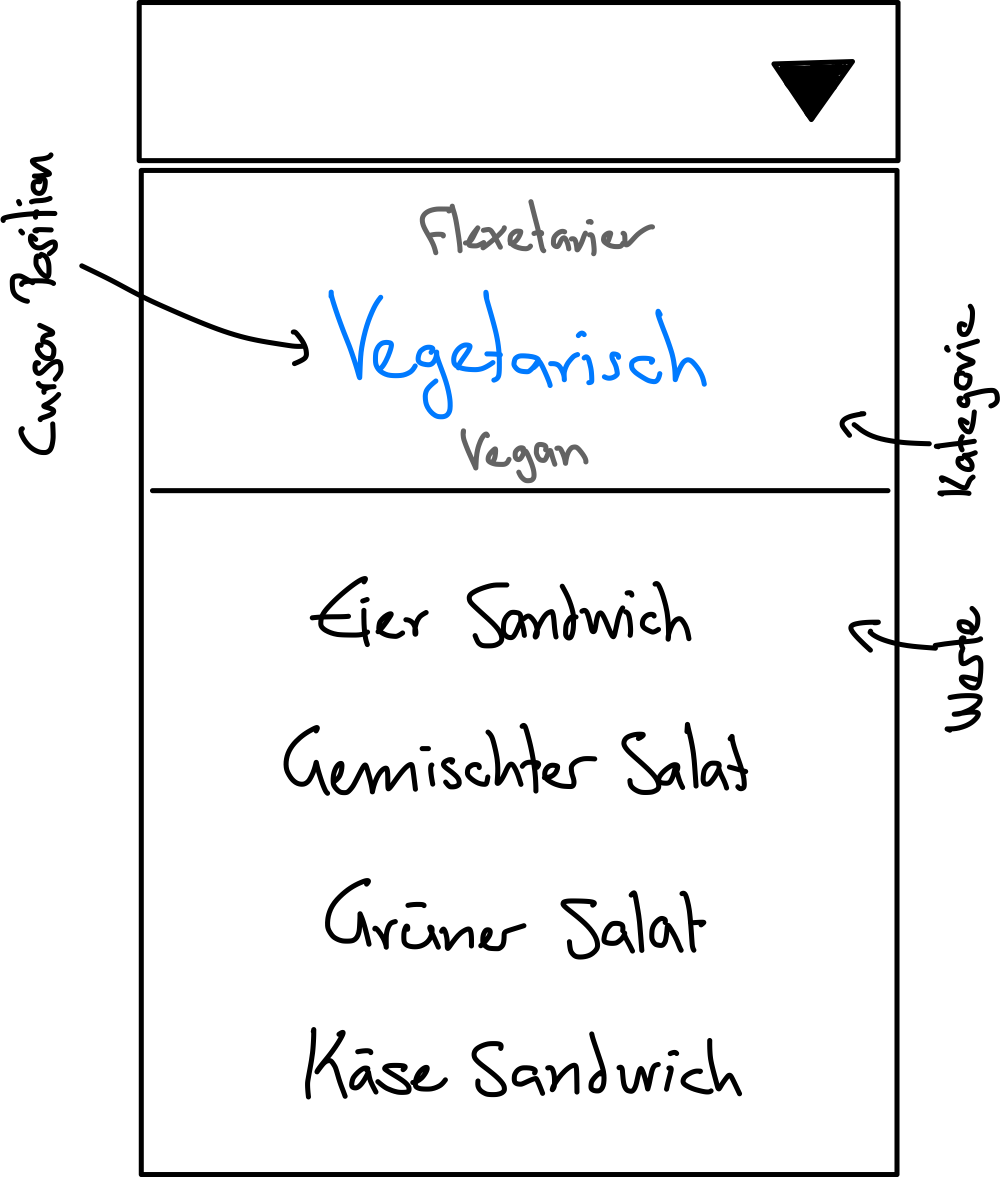
\includegraphics[width=60mm]{future-ui.png}
    \caption{Mögliches UI mit Zeilen-Aufbau}
    \label{img:futureUi}
\end{figure}

Die entstandenen als auch zukünftige UI-Projektoren lassen sich mit unterschiedlichen Interaktionen verbinden. 
Dabei ist es hilfreich, verschiedene Interaktions-Projektoren\footnote{
    Projektoren, die nur die Tastatur-Interaktion definieren
} zu bieten. 


\subsection{Weitere Interaktions-Projektoren}
\label{sec:moreInteraction}

Neue UI-Projektoren lassen sich nicht ausnahmslos mit den bestehenden Tastatur-Inter\-aktionen kombinieren. 
Zudem ist nicht in jeder Situation erwünscht, dass die Cursor Position die Selektion beeinflusst. 
Weitere Projektoren können neue, eventuell UI-Projektor spezifische Interaktionen bieten. 

Ein Interaktions-Projektor kann das Auswahlkomponente bezogene Undo und Redo enthalten. 
Diese Funktion bietet an, eine geänderte Auswahl rückgängig zu machen oder zu wiederholen. 


\subsection{Spezifische Auswahlkomponenten und Erweiterungen}
\label{sec:specificComponents}

Zukünftig besteht die Möglichkeit Auswahlkomponenten für spezielle Anwendungsfälle zu erstellen. 
Ein altbekanntes Beispiel ist die Auswahl eines Datums mit Tag, Monat und Jahr. 
Dabei kann weitere Logik zur Kontrolle der möglichen Werte zum Einsatz kommen. 

Das Erweitern der Multiselect-Funktionalität führt die Anpassung mehrerer Subkomponenten mit sich. 
Es betrifft die Implementation von der \codestyle{SelectComponent} bis hin zu der \codestyle{columnOptionsComponent}. 
Eine mögliche neue Single-Select Komponente bietet die Funktionalität mehrere Kategorien auswählen zu können. 
Hierbei ist zu unterscheiden, ob die ausgewählten Kategorien als AND- oder OR-Verknüpfung zu verstehen sind. 


\subsection{Performance verbessern und mögliche Datenmenge erhöhen}
\label{sec:betterPerformance}

Die \codestyle{SelectComponent} garantiert bis 5'000 Werte eine annehmbare\footnote{
    Ladezeit < 500ms bis die Webseite fertig geladen ist
} Ladezeit. 
Diese Performance lässt sich weiter optimieren. 
Zudem führen diese Verbesserungen dazu, dass sich eine noch höhere Anzahl Optionen anwenden lässt. 
Eine Kombination der Auswahlkomponente mit der Lazy Table des Kolibri ermöglicht eine optimierte Performance. 
Denn die Lazy Table kann eine Datenmenge von über 100'000 Werte verwalten. 


\subsection{Accessability verbessern}
\label{sec:betterAccessability}

Die entstandene Auswahlkomponente ist nur für nicht beeinträchtigte Menschen optimiert. 
Zukünftig ist die Komponente noch für Screen-Reader und somit für Blinde zu ergänzen. 
Die getroffenen Styles benötigen ein Testing mit Sehbeeinträchtigten, um die Accessability garantieren zu können. 
Dazu zählt zum Beispiel die bekannte Rot-Grün-Schwäche. 


\subsection{Abschliessende Bemerkungen}
\label{sec:endSumup}

All diese Erweiterungen und Verbesserungen zielen darauf ab, die Auswahlkomponente für alle Endnutzer zugänglich zu machen und eine angenehme Benutzung zu ermöglichen. 
Zudem soll die \codestyle{SelectComponent} einfach in jeden bestehenden JavaScript Code einzubinden sein. 
Anschliessend an diese Arbeit steht die Integration in das Toolkit Kolibri an. 


% listings
\chapter*{Glossar}
\addcontentsline{toc}{chapter}{Glossar}
\label{chap:glossary}

\newcommand{\glossarywithTitle}{0.23\textwidth}
\newcommand{\glossarywith}{0.76\textwidth}

% \vspace*{-1cm}
\begin{table}[!ht]
    \centering
    \rowcolors{2}{white}{gray!20}
    \footnotesize
    \begin{adjustbox}{max width=\textwidth}
        \begin{tabular}{ p{\glossarywithTitle} | p{\glossarywith} }
            \bf{Begriff} & \bf{Beschreibung} \\
            \hline \hline
            \bf{Aktuelle Browser} & \tbbr{
                Edge: Version 127 (Windows) \\
                Chrome: Version 127 (Windows / Mac) \\
                Firefox: Version 128 (Windows / Mac) \\
                Safari: Version 17.5 (Mac)
            } \\
            \hline
            \bf{ARIA-Rolle} & Accessible Rich Internet Applications Role.
                Sie definiert die Bezeichnung oder Funktion eines HTML-Elements.
                Sie dient als Markierung für Struktur und erweitert die Bedienbarkeit für u. a. Screenreader. \\
            \hline
            \bf{Ausgrauen} & Das Element erscheint in Grautönen mit eher schwachem Kontrast. \\
            \hline
            \bf{Client-Side} & Direkt im Browser. 
                Aktionen sehen den Server nie und bleiben im Browser. 
                Der Code ist direkt auf der HTML-Seite eingebunden. 
                In Zusammenhang mit Formularen erfährt der Server nichts von der Client-Side-Validierung. \\
            \hline
            \raggedright \bf{Digital Native} & Personen, die in der digitalen Welt aufgewachsen sind. \\
            \hline
            \raggedright \bf{Do-Nothing-Implementation} & 
                Implementation, welche als Stellvertreter z. B. beim Null-Object-Pattern dient. 
                Eine Funktion mit einer solchen Implementation führt nichts aus und hat keine Seiteneffekte. \\
            \hline
            \raggedright \bf{Dropdown-Komponente} & Synonym für Auswahlkomponente. \\
            \hline
            \bf{Endanwender} & Ein Nutzer, der die neue Komponente ausfüllt. \\
            \hline
            \bf{Hovern} & Mit der Maus über ein Element fahren. \\
            \hline
            \bf{Immutable} & Unveränderbar. Objekte sind nicht überschreibbar. \\
            \hline
            \bf{Kategorie} & Gruppierung der Optionen. 
                Das Selektieren einer Kategorie in einer \codestyle{Select\-Component} reduziert die Anzahl der Optionen. 
                Die Komponente zeigt nur noch Optionen an, welche der Kategorie / Gruppe zugewiesen sind. \\
            \hline
            \bf{KISS} & Keep it Simple and Stupid. 
                Ein Prinzip der Programmierung, in welcher alles möglichst einfach zu halten ist. 
                Einfache und kurze Codestücke minimieren das Risiko von Fehlern und Unverständlichkeit. \\
            \hline
            \bf{Multiselect} & 
                Auswahlkomponente (HTML \codestyle{select} Element), bei welcher mehrere Werte selektierbar sind. 
                Bei der Selektion einer zweiten Option hebt sich die vorherige Auswahl nicht auf. 
                Auf Desktop-Browsern muss jedoch die passende Taste bei der Auswahl gedrückt sein, damit sich die Selektion erweitert. \\
            \hline
            \bf{Regex} & Regular Expression. 
                Beschreibt eine Zeichenkette. 
                Syntaktische Regeln helfen bei der Verarbeitung von Texten. \\
            \hline
            \raggedright \bf{Separation of Concern} & 
                Ein Prinzip, welches in der Programmierung beim Aufteilen eines Programmes zur Anwendung kommt. 
                Jede Komponente besitzt nur eine Aufgabe. 
                Dadurch entsteht ein modularer Aufbau. \\
            \hline
            \bf{Single-Select} & 
                Auswahlkomponente (HTML \codestyle{select}-Element), bei welchem nur ein Wert selektierbar ist. 
                Bei der Selektion einer zweiten Option hebt sich die vorherige Auswahl auf. \\
            \hline
            \bf{Spiegelstrich} & 
                Ein Strich, welcher sich auf der linken Seite eines Elements bzw. einer Option befindet. 
                Der Strich ist vertikal und dient zum Hervorheben des Elements. \\
            \hline
            \bf{Togglen} & Auf- bzw. zuklappen des Popovers. \\
            \hline
            \bf{Triggern} & Auslösen eines Events. \\
            \hline
            \bf{UI/UX-Design} & Design der Benutzeroberfläche und der Benutzererfahrung. \\
            \hline
            \raggedright \bf{Vorarbeit/ vorangegangenes Projekt/ Vorgängerprojekt} & 
                Semesterarbeit bevor die Bachelorarbeit beginnt. 
                In dieser Arbeit finden Vorbereitungen auf die kommende Bachelorarbeit statt. 
                Die FHNW nennt diese Arbeit intern Informatik-Projekt 5 – kurz IP5. 
                Das Resultat des Projekts ist im Kapitel \nameref{sec:countryChoice} beschreiben. \\
            \hline
            \bf{Workaround} & 
                Alternativer Code, wenn der Ursprüngliche nicht funktioniert. 
                Eine Möglichkeit, ein Problem zu umgehen. \\
            \hline
            \hline
            \raggedright \bf{* Tabellen-Fussnote} & Bemerkung gilt für die ganze Tabelle. \\
            \hline
        \end{tabular}
    \end{adjustbox}
\end{table}


\setcounter{biburllcpenalty}{9000}
\emergencystretch=1em
\printbibliography[title={Quellenverzeichnis}]
\addcontentsline{toc}{chapter}{Quellenverzeichnis}

\listoffigures
\addcontentsline{toc}{chapter}{Abbildungsverzeichnis}

\lstlistoflistings
\addcontentsline{toc}{chapter}{Codeverzeichnis}

\listoftables
\addcontentsline{toc}{chapter}{Tabellenverzeichnis}

\appendix
\chapter{Aufgabenstellung}
\label{chap:task}


\includepdf[pages=-]{../appendix/24FS_IMVS17_Generalisierte_Auswahlkomponente_Kolibri.pdf}


\chapter{Existierende Komponenten - Bilder}
\label{chap:existingImgs}

\section*{Select}
\graphicspath{ {./img/select/} }
\import{../appendix}{existingSelectImgs.tex}
\graphicspath{ {./img/} }

\clearpage
\section*{Datalist}
\graphicspath{ {./img/datalist/} }
\import{../appendix}{existingDatalistImgs.tex}
\graphicspath{ {./img/} }


\chapter{User Test für Programmierer}
\label{chap:userTestProgrammers}

\section*{Code}

\lstinputlisting[style = htmlcssjs, caption = \texttt{userTesting.js}, label = code:userTestingJs]{../userTest/userTesting.js}
\lstinputlisting[style = htmlcssjs, caption = \texttt{userTesting.html}, label = code:userTestingHtml]{../userTest/userTesting.html}
\lstinputlisting[style = htmlcssjs, caption = \texttt{starter.js}, label = code:starterJs]{../userTest/starter.js}
\begin{lstlisting}[style = htmlcssjs, caption = \texttt{dataService.js}, label = code:dataServiceJs]
export {
    getAllContinents,
    getCountries,
    getCountriesChDeAt,
    getRegionsByCountry,
    getRegionsByCountryChDeAt,
    getYearsByDecade,
    getDecades,
    getLunchTypes,
};

/** @type { (String) => String } */
const getAllContinents = () => [
    ...new Set(...allCountriesWithContinent.map((country) => country.continent)),
];

/** @type { (String) => String } */
const getCountries = (continent) =>
    allCountriesWithContinent
        .filter((e) => e.continent === continent || !continent)
        .map((country) => country.country);

/** @type { (String) => String } */
const getRegionsByCountry = (country) =>
    allRegionsWithCountry
        .filter((e) => e.country === country || !country)
        .map((region) => region.region).sort();

/** @type { (String) => String } */
const getCountriesChDeAt = () => ["Switzerland", "Germany", "Austria"];

/** @type { (String) => String } */
const getRegionsByCountryChDeAt = (country) =>
    allRegionsWithCountry
        .filter(
            (e) => e.country === country || (!country && ["CH", "DE", "AT"].includes(e.code))
        )
        .map((region) => region.region).sort();

/** @type { (String) => String } */
const getYearsByDecade = (decade) => {
    const decadeStart = decade?.slice(0, 3);
    const data = [...Array(90).keys()].map((e) => e + 1930 + "");
    return data.filter((e) => !decade || e.startsWith(decadeStart));
};

/** @type { (String) => String } */
const getDecades = () => [...Array(9).keys()].map((e) => e * 10 + 1930 + "'s");

/** @type { (String) => String } */
const getLunchTypes = () => ["all", "vegetarian", "vegan", "flexetarian", "gluten-free", "lactose-free"];

/* data tables for `allCountriesWithContinent` and `allRegionsWithCountry` */
/* Link: https://github.com/fhnw-ramonamarti/fhnw-ramonamarti.github.io/blob/main/ip6/userTest/dataService_old.js */
\end{lstlisting}


\section*{Resultate}
\noindent
\textbf{Siehst du irgendwo Verbesserungspotenzial?}

\noindent 
- Detail: numberOfColumns ist etwas "verbose"
\\
- Doku: In der Code Doku von SelectComponent dürfte der Return Value besser beschrieben werden (welches Array Element ist was). 
Das wird erst in den Anwendungsbeispielen klar. 

Keyboard navigation. Using keyboard to narrow down possible categories/values (maybe fuzzy searching), 
otherwise it takes me longer to find something than compared to a standard dropdown, even if the list there is bigger.

ich finde es etwas unintuitiv beim SelectComponent neben den offensichtlich verständlichen selectAttriutes (labl, name, numberOfColumns) noch ein Callback mitzugeben.   
ich hätte mir mehr beschreibung gewünscht wie ich die komponente verwenden muss. (ich musste eher dannach suchen.)

Bessere Dokumentation war verwirrend (Code).

Automatisches Schliessen der Komponente nach der Auswahl würde ich praktisch finden.

Es würde helfen, wenn die Types im JSDOC spezifiziert wären und wenn die Library eingebunden wäre. 
Dann wäre die Dokumentation leichter auffindbar.

War mir am Anfang nicht klar dass was SelectComponent() zurückgibt und ob das Input-element sowie dass label-element selbst erstellt werden soll. 
Danach war es intuitiv anzuwenden.

 \\

\noindent
\textbf{Bemerkung}

ich persönlich hatte zu beginn schwierigkeiten zu verstehen wie das framework funktioniert. 
die beschreibung für die tasks (ab task2) sind zum teil etwas unklar 
\\
=> The value data is provided by the function `Service.getRegionsByCountry()`, 
the categories are provided by the function `Service.getCountries()`  
\\
=> RegionsByCountry muss man noch das Country mitgeben. 
Hätte in der beschreibung drinstehen können.

Nitpicking: while I see why the component is imported from a URL for the user tests, it makes it hard to use on a spotty network.

 \\

Isch s selectAttributes `numberOfColumns` wörklich nötig? 
Vo mir uus gseh, chönt mer `numberOfColumns` vo `serviceCallbacks.length` ableite...?
\\ Ehr hend nah recht es performance Problem wenn d liste lang isch...
Dur s implementiere vo Task 2.2 brucht d websiite ca. 5 sekunde zum lade (rein Javascript execution). 
Das liht ned ahm Javascript, sondern am HTML rendering sowiit ih gseh ha. 
Ha suscht nah e Performance Trace gmacht wo mer in Chrome chan drii lade ahhghänkt.
\\ Isch betz speziell, dass `serviceCallbacks` array in vercherter reihefolg muen drii geh werde wies denne ahhzeigt wird...
\\ Wenn mer 2 Kollone het, aber rechts ke uuswahl, de chan mer au nüt uuswähle... 
Ja isch z erwarte aber isch au ih de Demo vorhande
\\ För mich isch ned immer klaar gsii, wenns nah meh optione unde oder obedraa het. 


\graphicspath{ {./img/userTests/} }
\begin{figure}[!p]
    \centering
    \begin{minipage}[b]{0.6\textwidth}
        \centering
        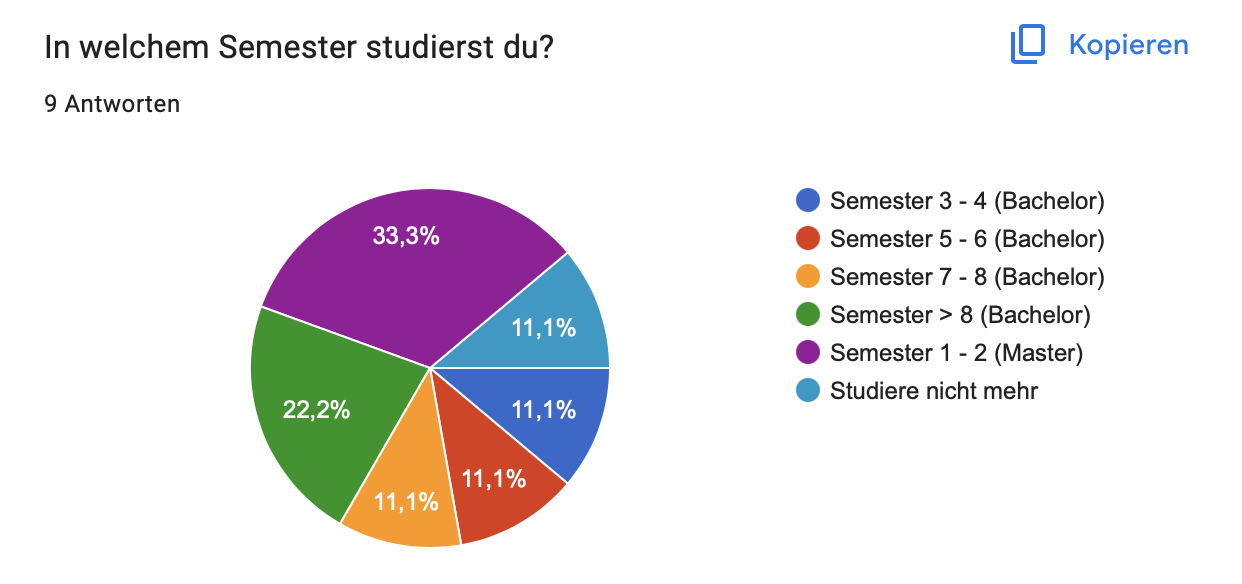
\includegraphics[width=\textwidth]{semester9.png}
        \caption{User Test Programmierer Frage 1}
        \label{img:userTestSemester}
    \end{minipage}
    \begin{minipage}[b]{0.6\textwidth}
        \centering
        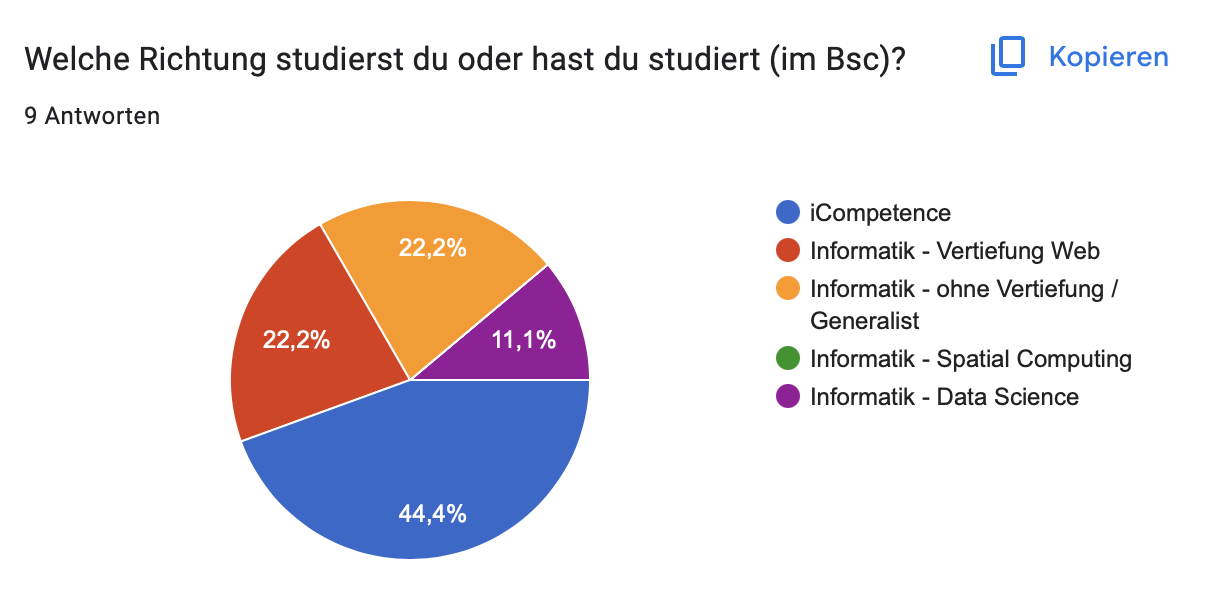
\includegraphics[width=\textwidth]{richtung9.png}
        \caption{User Test Programmierer Frage 2}
        \label{img:userTestStudy}
    \end{minipage}
    \begin{minipage}[b]{0.6\textwidth}
        \centering
        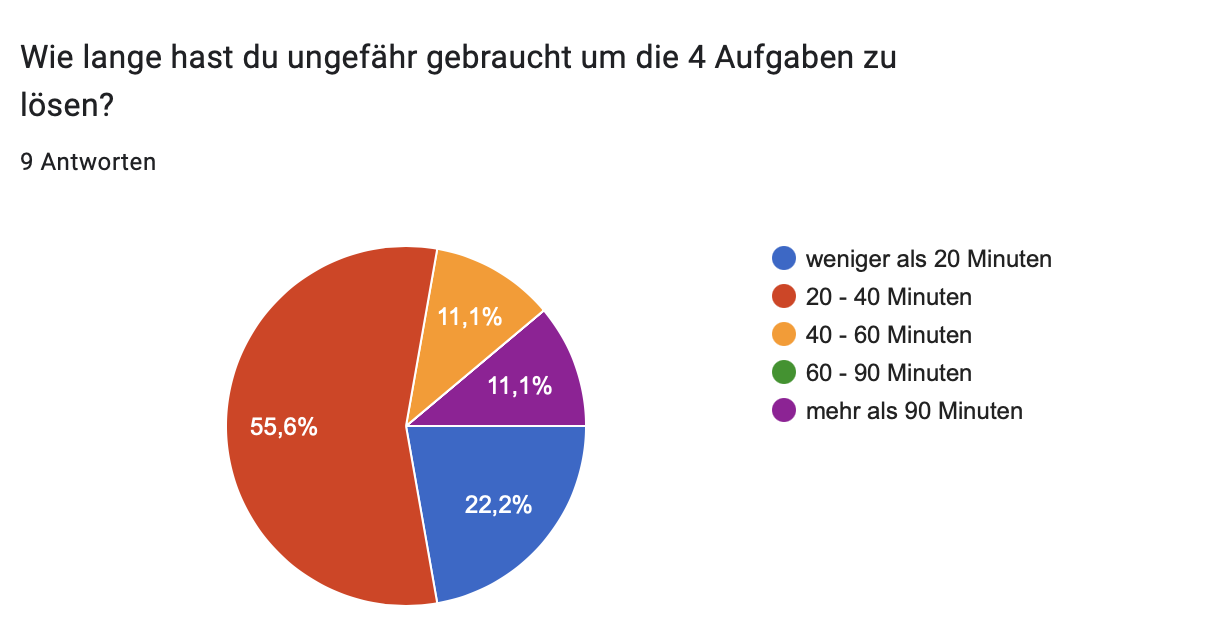
\includegraphics[width=\textwidth]{dauer9.png}
        \caption{User Test Programmierer Frage 3}
        \label{img:userTestDuration}
    \end{minipage}
    \begin{minipage}[b]{0.6\textwidth}
        \centering
        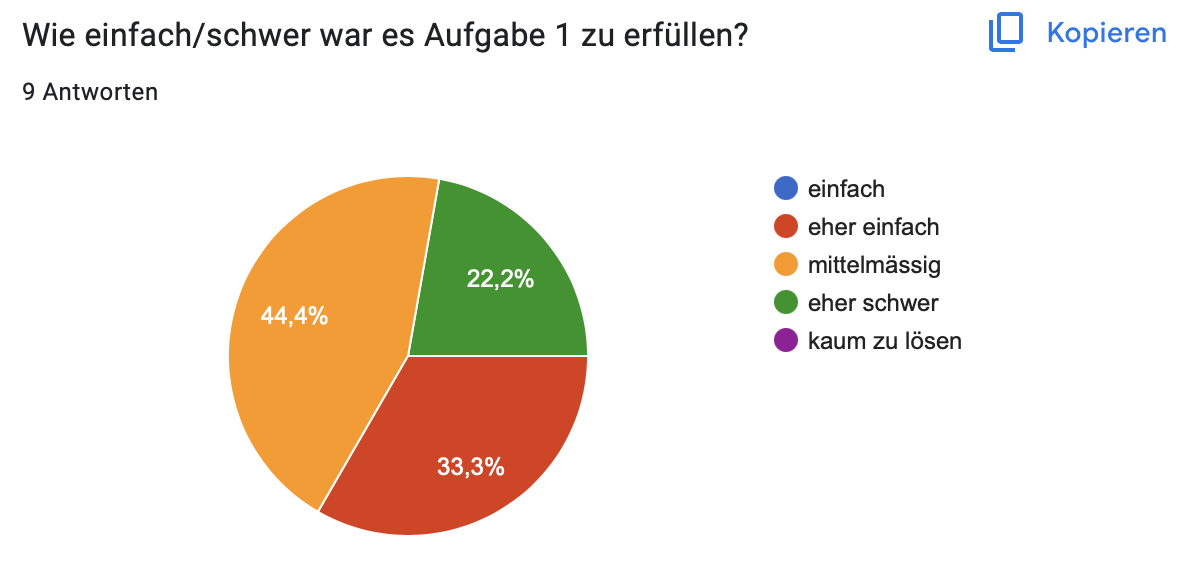
\includegraphics[width=\textwidth]{a1_9.png}
        \caption{User Test Programmierer Frage 4}
        \label{img:userTestA1}
    \end{minipage}
\end{figure}

\begin{figure}[!p]
    \centering
    \begin{minipage}[b]{0.6\textwidth}
        \centering
        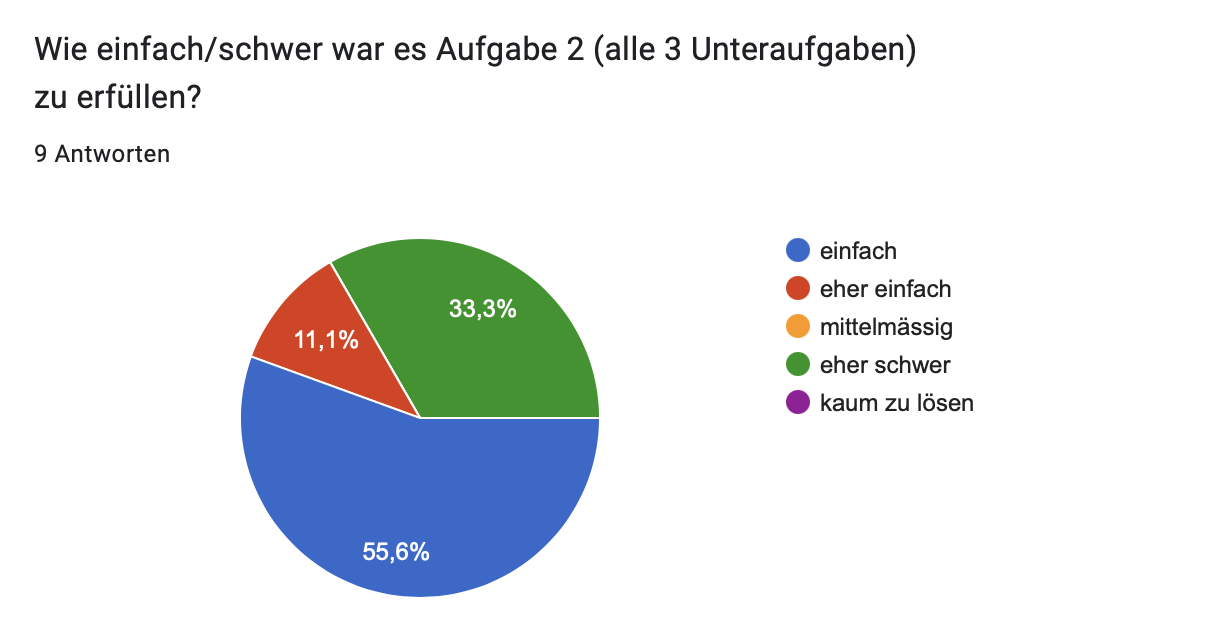
\includegraphics[width=\textwidth]{a2_9.png}
        \caption{User Test Programmierer Frage 5}
        \label{img:userTestA2}
    \end{minipage}
    \begin{minipage}[b]{0.6\textwidth}
        \centering
        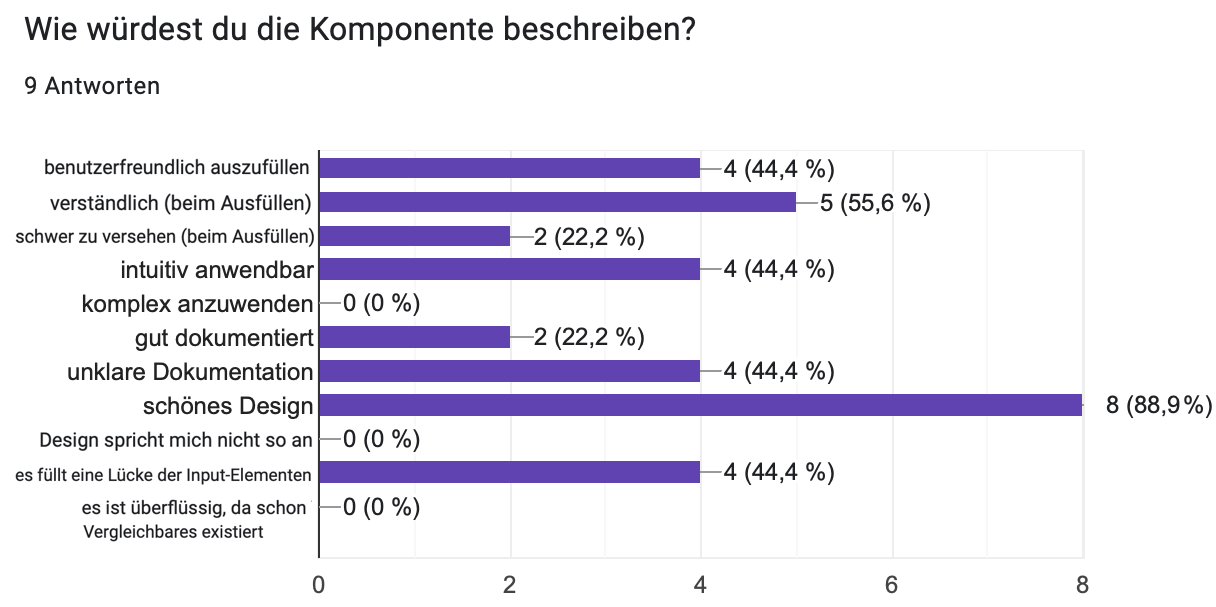
\includegraphics[width=\textwidth]{desc9.png}
        \caption{User Test Programmierer Frage 6}
        \label{img:userTestDesc}
    \end{minipage}
    \begin{minipage}[b]{0.6\textwidth}
        \centering
        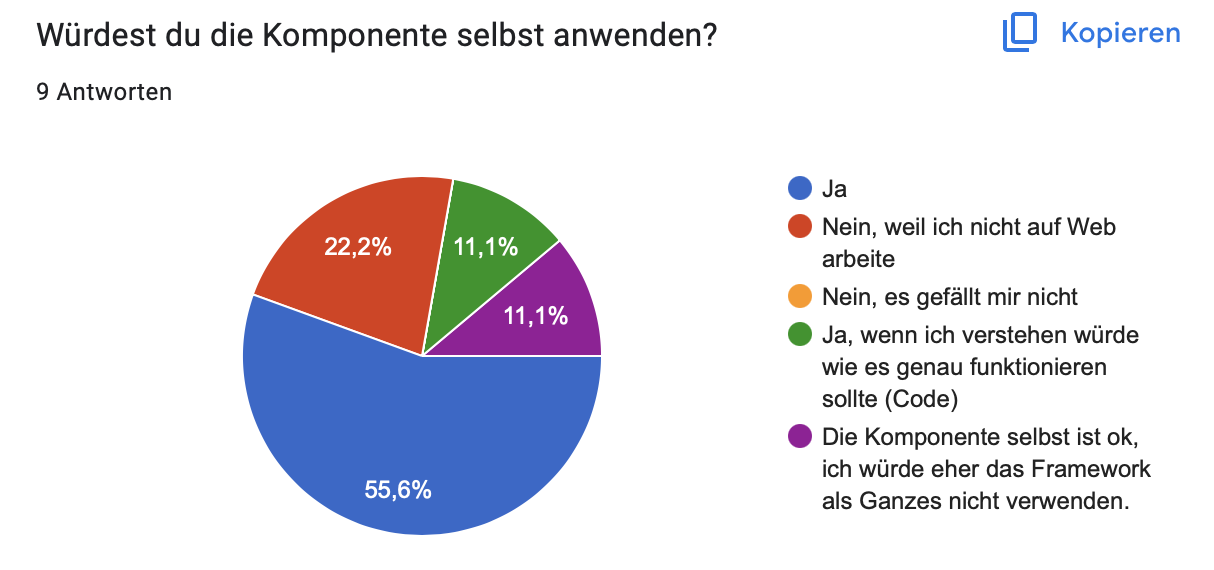
\includegraphics[width=\textwidth]{anwenden9.png}
        \caption{User Test Programmierer Frage 7}
        \label{img:userTestUsage}
    \end{minipage}
\end{figure}

\graphicspath{ {./img/} }

\chapter{Personas}
\label{chap:perosnas}

\begin{landscape}
    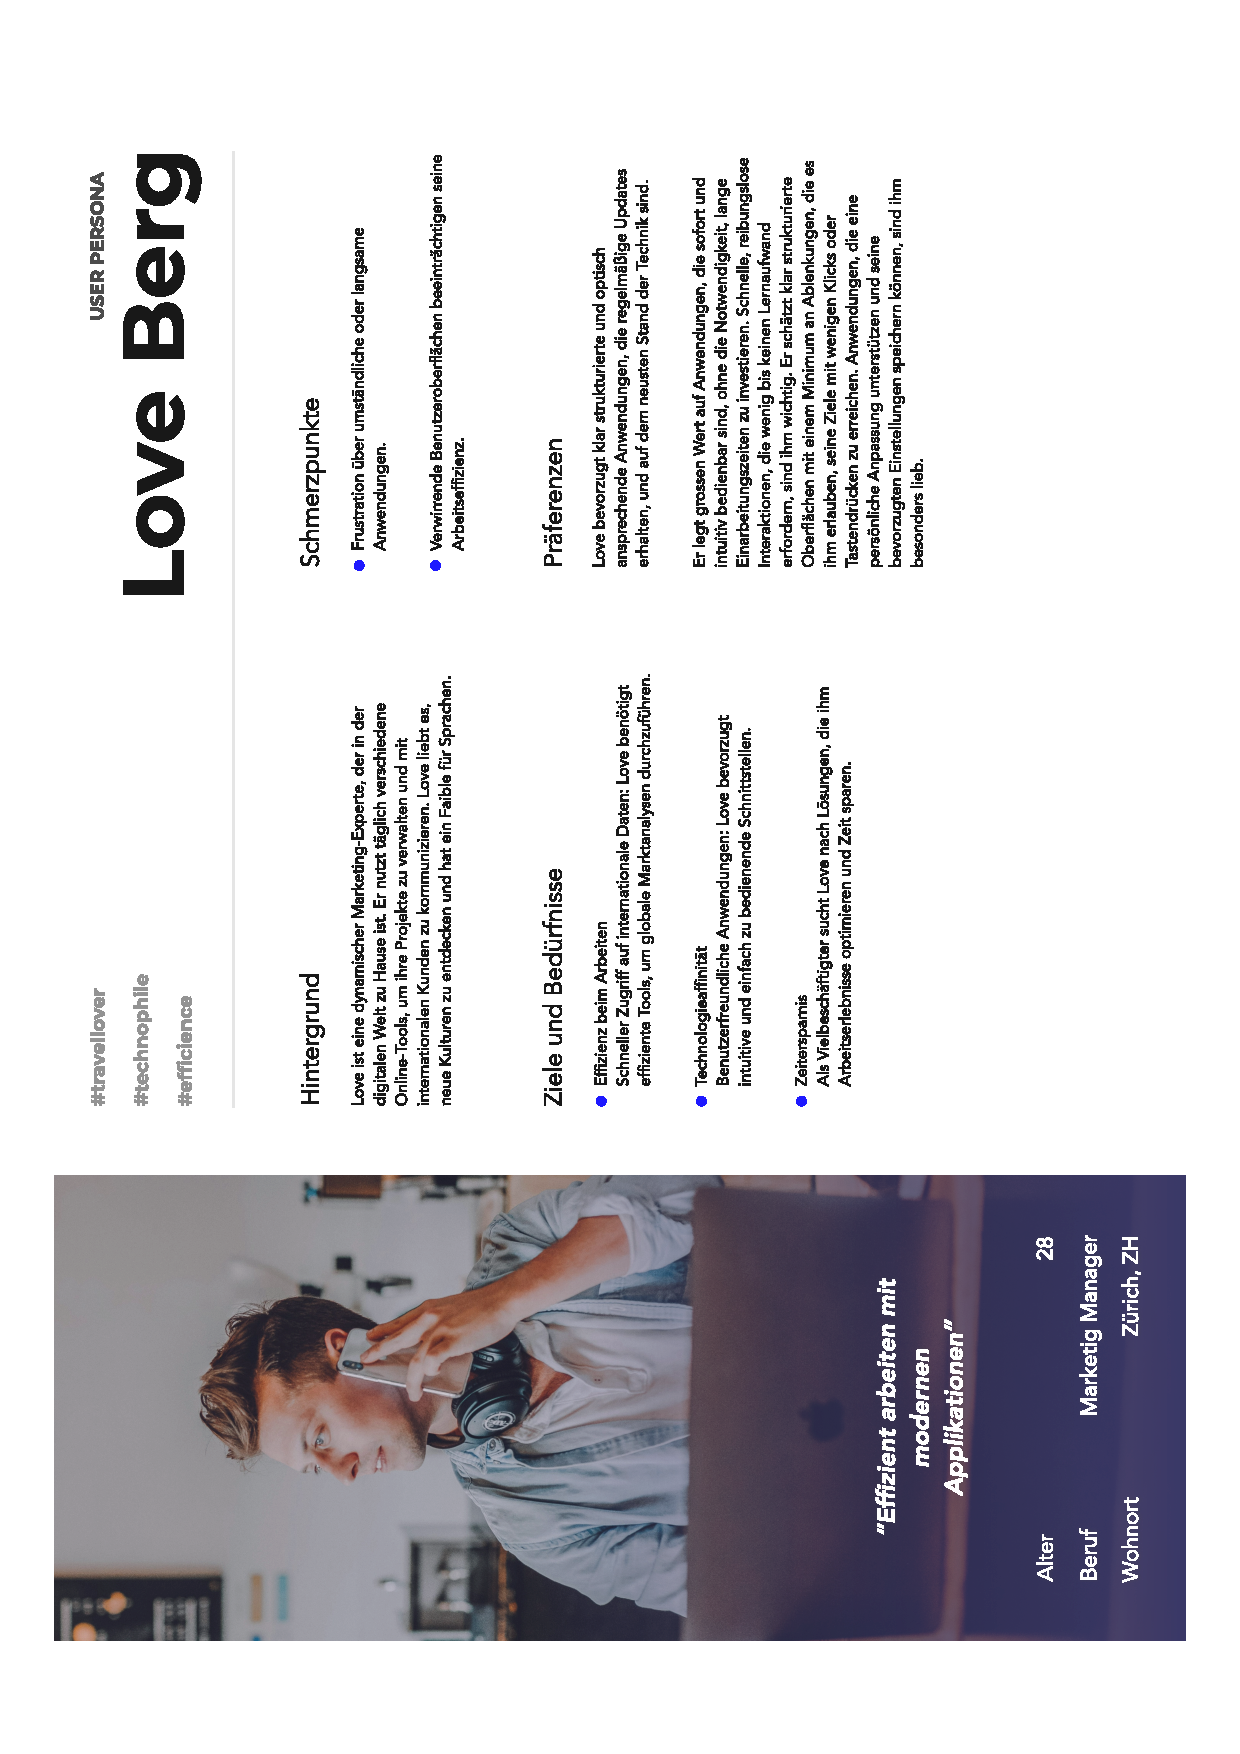
\includepdf[pages=-]{../appendix/Persona_User.pdf}
    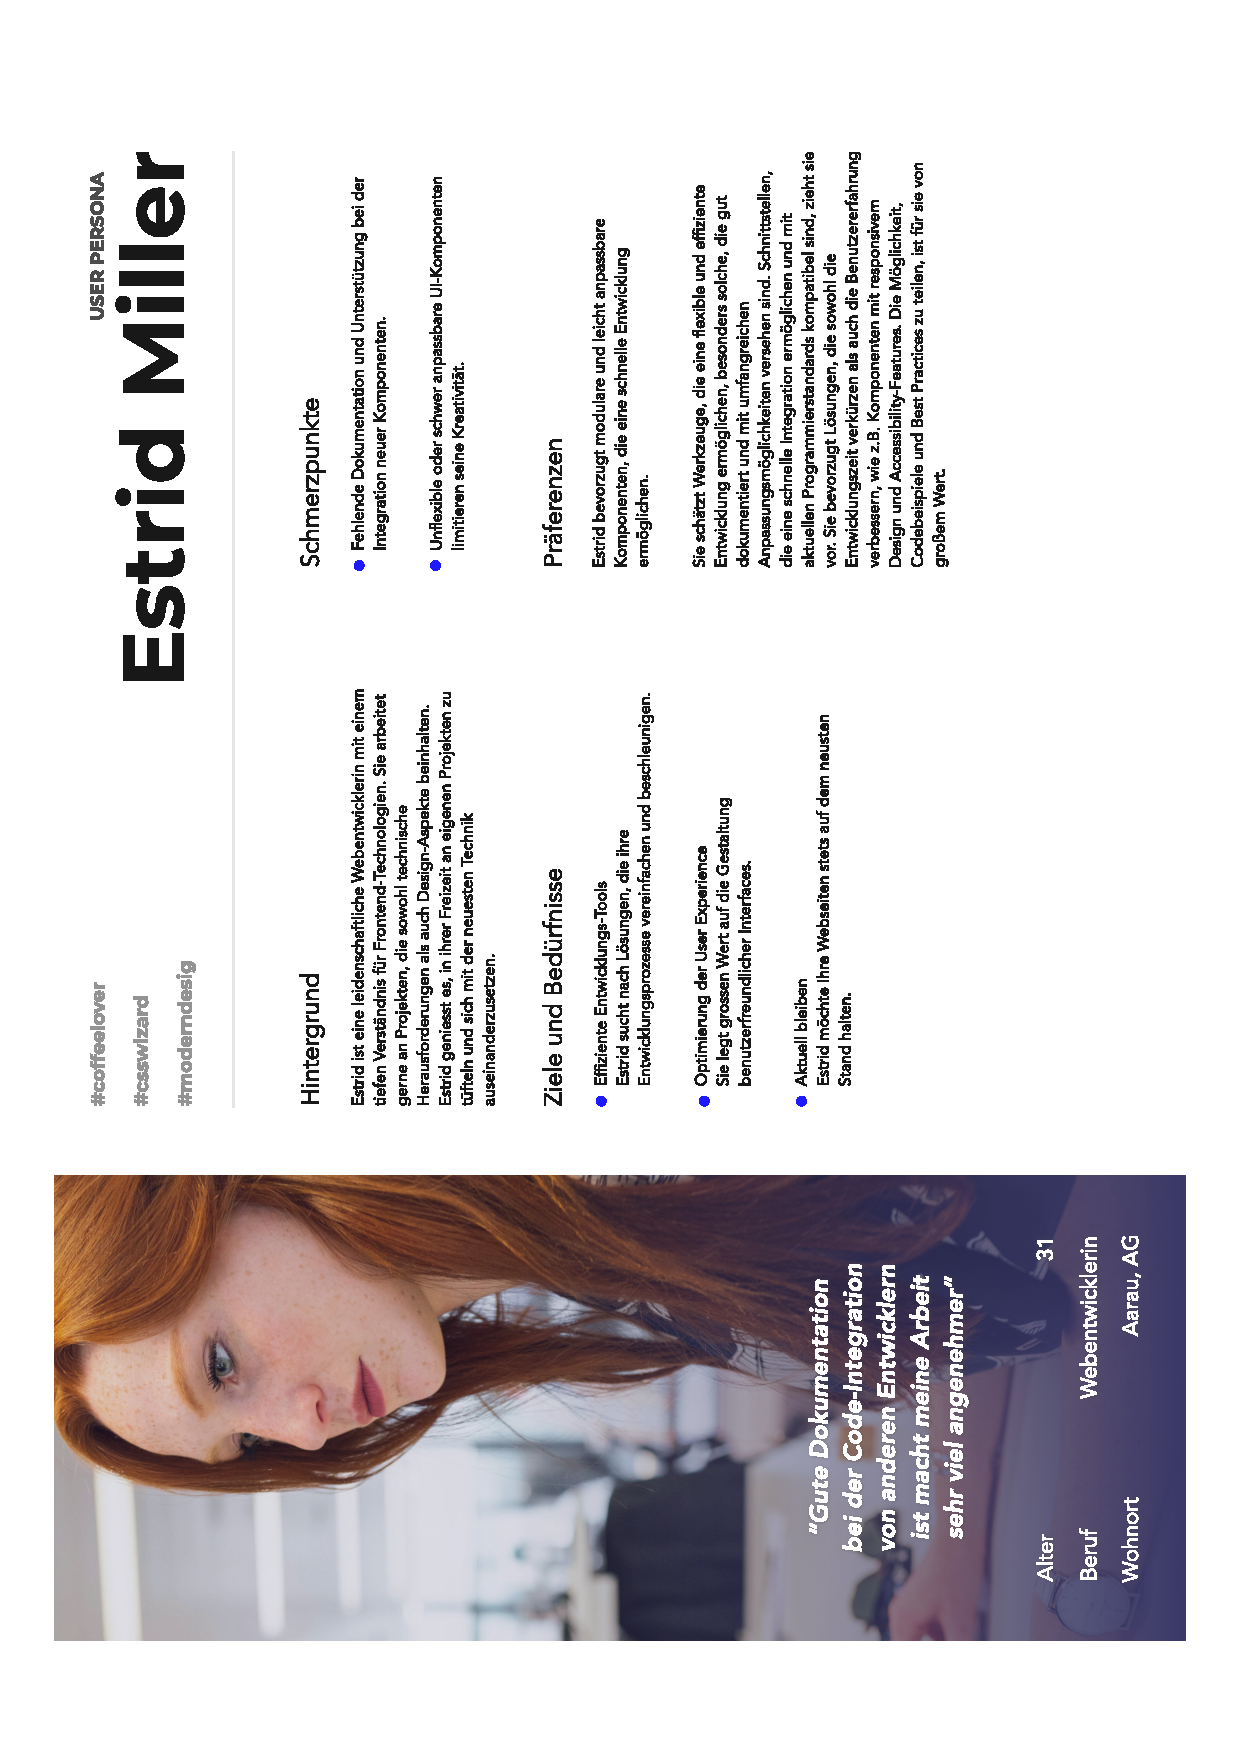
\includepdf[pages=-]{../appendix/Persona_Dev.pdf}
\end{landscape}

% \chapter{API} % todo write api for usage component
% \label{chap:api}


\end{document}
